\chapter{Загадки Почайны}

Зачем после Боричева понадобилась целая глава о реке Почайне? А без нее дальше никак.

Про Почайну обычно пишут или кратко, или затрагивают только низовье её около Подола, основываясь на ставших уже хрестоматийными словах Берлинского да Закревского, а в качестве приправы величают словом «летописная». Ясно, что Почайной называли то ли большущий приток, то ли рукав Днепра, по правую его сторону.

Большинство краеведов указывают, как на остатки Почайны, на цепь здоровенных, раздувшихся, соединенных друг с другом озер, питаемых за счет правобережных ручьев и рек, выведенных в озера из коллекторов. Этим проточным озерам невесть кем дано общее имя Опечень. А по одному: Минское, Луговое, Богатырское, Кирилловское, Иорданское, Вербное. Наконец, портовый залив Подольской Гавани. И добавляют, что прежде река простиралась до памятника Магдебургскому праву, отделенная от Днепра песчаной косой.

Это очень упрощенное и частично ошибочное современное понимание Почайны. Попробуем разобраться, какой была река раньше и как это соотносится с положением нынешним.

Ближе к устью Десны, от неё на юг идет рукав Черторыя (Десенка), впадающий в Днепр аж в районе Гидропарка. Нам так далеко не надо. Передвинемся к самому устью Десны. Между Черторыей (с востока), оставшимся отрезком Десны (с севера) и Днепром (с запада), от устья Десны к северу лежит большущий остров Муромец, ранее Муравец, где был одноименный хутор. Сейчас на острове – Парк Дружбы Народов, переходящий, ближе к устью Десны, в луговину с рощами.

На север от Московского моста – Муромец, а на юг – другой остров, Труханов. К Муромцу относится и пляж у моста. Если верить трехверстовой карте Шуберта, местами весьма неточной, в середине 19 века правый берег Днепра подходил к этому пляжу, а Днепр был сдвинут восточнее.

Ныне, от Муромца через Днепр, на правом берегу оного, находятся жилые массивы Минский и Оболонь, скучно пронумерованные микрорайоны, построенные на поднятых гидронамывом песках.  Старая местность Оболонь похоронена под ними на глубине 4-5 и более метров. Далее к западу – цепь озер Опечень, затем снова равнина Оболони, и потом уж возвышенность – Приорка, Куренёвка, Кирилловские высоты.

На месте восточной части Оболони, то бишь к востоку от Опечени, раньше было два крупных острова.

Северный остров назывался Чачин (Чичин), начинался на уровне устья Десны и завершался около северной части теперешнего залива Оболонь. С юга Чачина был проток от Днепра. Проток сей, подписанный на картах то Пробивицей (не путать с Пробивцем на Труханове), то Стариком, шел на запад и затем разделялся надвое. Одна часть его отклонялась, огибая Чачин, на север. А другая – дальше к западу и соединялась с Почайной.

От Чачина на юг лежал второй остров – суша между Почайной и Днепром. Часть Оболони.

По крайней мере в конце 17 века было две Почайны. Два разных водоема именовались одинаково. Основное русло первого водоема (назовем его Почайна-1) начиналось на широте современного озера Министерки (два с половиной километра южнее Вышгорода) и длилось на юг до Подола, чуть севернее коего соединялось с Днепром. Русло другой Почайны (Почайна-2) было обычным рукавом Днепра на протяженности Подола и несколько южнее его.

Как такое может быть с названием? Несколько ответов, не исключены и другие.

Первый – некогда была одна Почайна, с непрерывным руслом, потом распалась на две, но по старой памяти оба водоема продолжали называть как один.

Второй – «почайна», возможно, не личное имя реки, а слово, обозначавшее нечто. Значение утеряно. В том же 17 веке Почайна в документах зачастую упоминается не просто «Почайна», однако – Почайна кривая, или – Почайна песчаная, причем всё это относительно широт Почайны-1.

В летописях говорится просто о Почайне. Причем в древнейших списках – только единожды. Княгиня Ольга передает византийским послам слова для византийского же императора, что подарки последнему она отправит, только когда император лично постоит у нее в Почайне, как Ольга стояла в константинопольской гавани Суд: «А ще ты такоже постоиши у мене в Почайне, якоже аз в Суду, то тогда ти вдам». Можно ли из этого сделать вывод, где протекала Почайна при Ольге? Нельзя. Но без доводов полагают, что вдоль Подола.

Если это в самом деле так, любопытно сопоставить, что летописный «Ручай», о коем расскажу далее, и былинное именование Почайны – Пучай – отличаются одной лишь буквой. Не закралась ли ошибка в летописи? Не стал ли Пучай – Ручаем?

Существует также предание о крещении киевлян Владимиром Красно-Солнышко именно в Почайне, а не Днепре. Где это предание можно прочитать? В летописях? Старейшие летописи молчат о Почайне, кроме упоминания ее княгиней Ольгой. Эти летописи однако говорят про крещение в Днепре. Приведу выдержку из Ипатьевского списка:

\begin{quotation}
Наутрея же изииде Володимер с попы царицины и Корсуньскыми на Днепр, и снидеся бе-щисла людии: и влезоша в воду, и стояху ови до шее, а друзии до персий, младеи же от берега, друзии же младенци держаще, свершении же бродяху, попове же стояще молитвы творяху.
\end{quotation}

Несколько более новых списков вроде Холмогорского и Львовского противоречат этому. В последнем говорится:

\begin{quotation}
Наутрее же князь великий Владимер с попы царицыными и с Корсуньскими на реку на Почаю сниде. без числа люди; и влезоша в воду, и стояху в не йдо шеи, а другия до перси, млады же от берега [...]
\end{quotation}

А Николай Закревский в «Описании Киева»\cite{zakr01}цити\-рует некоторые списки Пролога, где о крещении при Владимире сказано:

\begin{quotation}
И сниде на Поцайну реку весь возраст муж и жен.... И оттоле наречется место то Святое, идеже ныне церкы Петрова.
\end{quotation}

«Ныне» это, если датировка книги верна, 13 век. В 13 веке на месте проведения обряда крещения стояла церковь Петрова, вдоль протекала Почайна, а место называли «Святым». В 19 веке «Святым местом», кажется более с подачи историков, чем по народной молве, именовали местность, овраг около источника Хрещатика (где памятник-колонна Магдебургскому праву, она же нижний памятник князю Владимиру), в коем, как пишет Максим Берлинский в «Кратком описании Киева» 1820 года издания\cite{berl01}, Владимир крестил своих сыновей.

Мы еще вернемся к этому Хрещатику или Крещатику. Напомню, что одноименная улица хотя и лежит в большом яру, это не давний Хрещатый (Крещатый яр). Улица подходит к Владимирскому спуску, и несколько ниже этого пересечения, в сторону Днепра за площадкой с колоннадой, открывается яр с большой лестницей, ведущей к памятнику-колонне Магдебургскому праву. Вот сей-то яр и есть Крещатый. А нынешний Крещатик это, как я полагаю, давняя Евсейкова долина.

Закревский отмечает, что в позднейших Прологах вместо церкви Петра, установленной по месту крещения киевлян, указана другая, «Мученику у Турова». А в Синопсисе 1674 года – «церковь во имя святаго мученика Турова». Так и тянет сопоставить это с летописной Туровой божницей, да упомянутой в давних документах «смуговиной Турец».

Про Турову божницу в источниках неизвестно ничего, кроме летописного сообщения за 1146 год, когда Игорь Ольгович звал киевлян на гору на Ярославль двор, а киевляне в то время собрали вече у Туровой божницы, вероятно где-то внизу. Вопреки популярным представлениям про «вече» – мол, собирался весь честной народ и решал государственные дела – в летописях есть подробность, что собирался не весь честной народ, но конный, стало быть люди зажиточные, либо военное сословие. Но это вопрос особый.

Кому же верить про крещение? Старейшим летописям? Тогда крестили в Днепре. Некоторым житиям из Пролога или поздним спискам летописей? Стало быть, в Почайне. А если взять житие Владимира из Степенной книги царского родословия, то там крестят в Днепре, и на месте проведения обряда ставят церковь «святаго мученика Турова».

Так какую церковь возвели? То же самое – выбирай что глянется.

А известно ли, где стояли эти храмы? Если не привязывать их современными рассуждениями к памятнику Магдебургскому праву, то следы приведут нас к улице Туровской, однако не современной, а той, что пролегала до пожара 1811 года. Турову божницу и схожую по названию церковь (а вероятно всего это одно и то же) следует искать около речушки Турца. К этому мы обратимся позже.

Почайна застолблена в былинах, как Пучай-река и Пучайка. Былины донесли нам древние имена киевских урочищ – Сорочинские горы (Кирилловские высоты), крест Леванидов, повезло и Почайне, но какой – первой или второй? Или в древности это был таки один непрерывный водоем?

Пора обратиться к картам, давним и самопальным. Я составил таковую, чтобы показать, как соотносится давнее русло Почайны-1 с современными озерами на Оболони и современным же руслом Днепра.

Сразу оговорюсь, что летописное русло Почайны восстановить невозможно, слишком сильно за это время изменилось русло Днепра. Гигантским полозом извиваясь в своей долине, он смешивал всё, влияя на попадающие в пойму водоемы.

Я использовал наложение друг на друга следующих карт – спутниковой за 2015 год, трехверстовки Шуберта середины 19 века, и плана русла Днепра около Киева за 1914 год.

Древнейший план Киева от полковника Ушакова, за 1695 год, где показано полное русло Почайны, на современную карту не накладывается по причине иных принципов построения плана Ушакова, весьма своеобразных, о чем еще скажу далее.

Точность наложения задействованных карт оцениваю как достаточную, поскольку они совпадают в различных местах, которые не менялись или слабо изменились за полтора столетия – это сетка улиц Подола, левобережное озеро Радунка, линия гор правого берега (в целом сохранившаяся на отрезке от Подола и южнее), известные монастыри. 

Однако к данным карты Шуберта отношусь настороженно – она сильно ошибается возле Троещины и на северо-восток оттуда, не исключены ошибки и на правом берегу.

Итак, карта отражает положения русла остатков Почайны на временном отрезке указанных выше планов, и пытается восстановить положение частей Почайны, упомянутых в документах 17-18 веков. Например, известный тогда пролив Ицун, соединявший Днепр и Почайну, в 1914 году представлял собой уже оторванное от Днепра озеро под названием Вицун.

\newpage
\vspace*{\fill}
\begin{center}
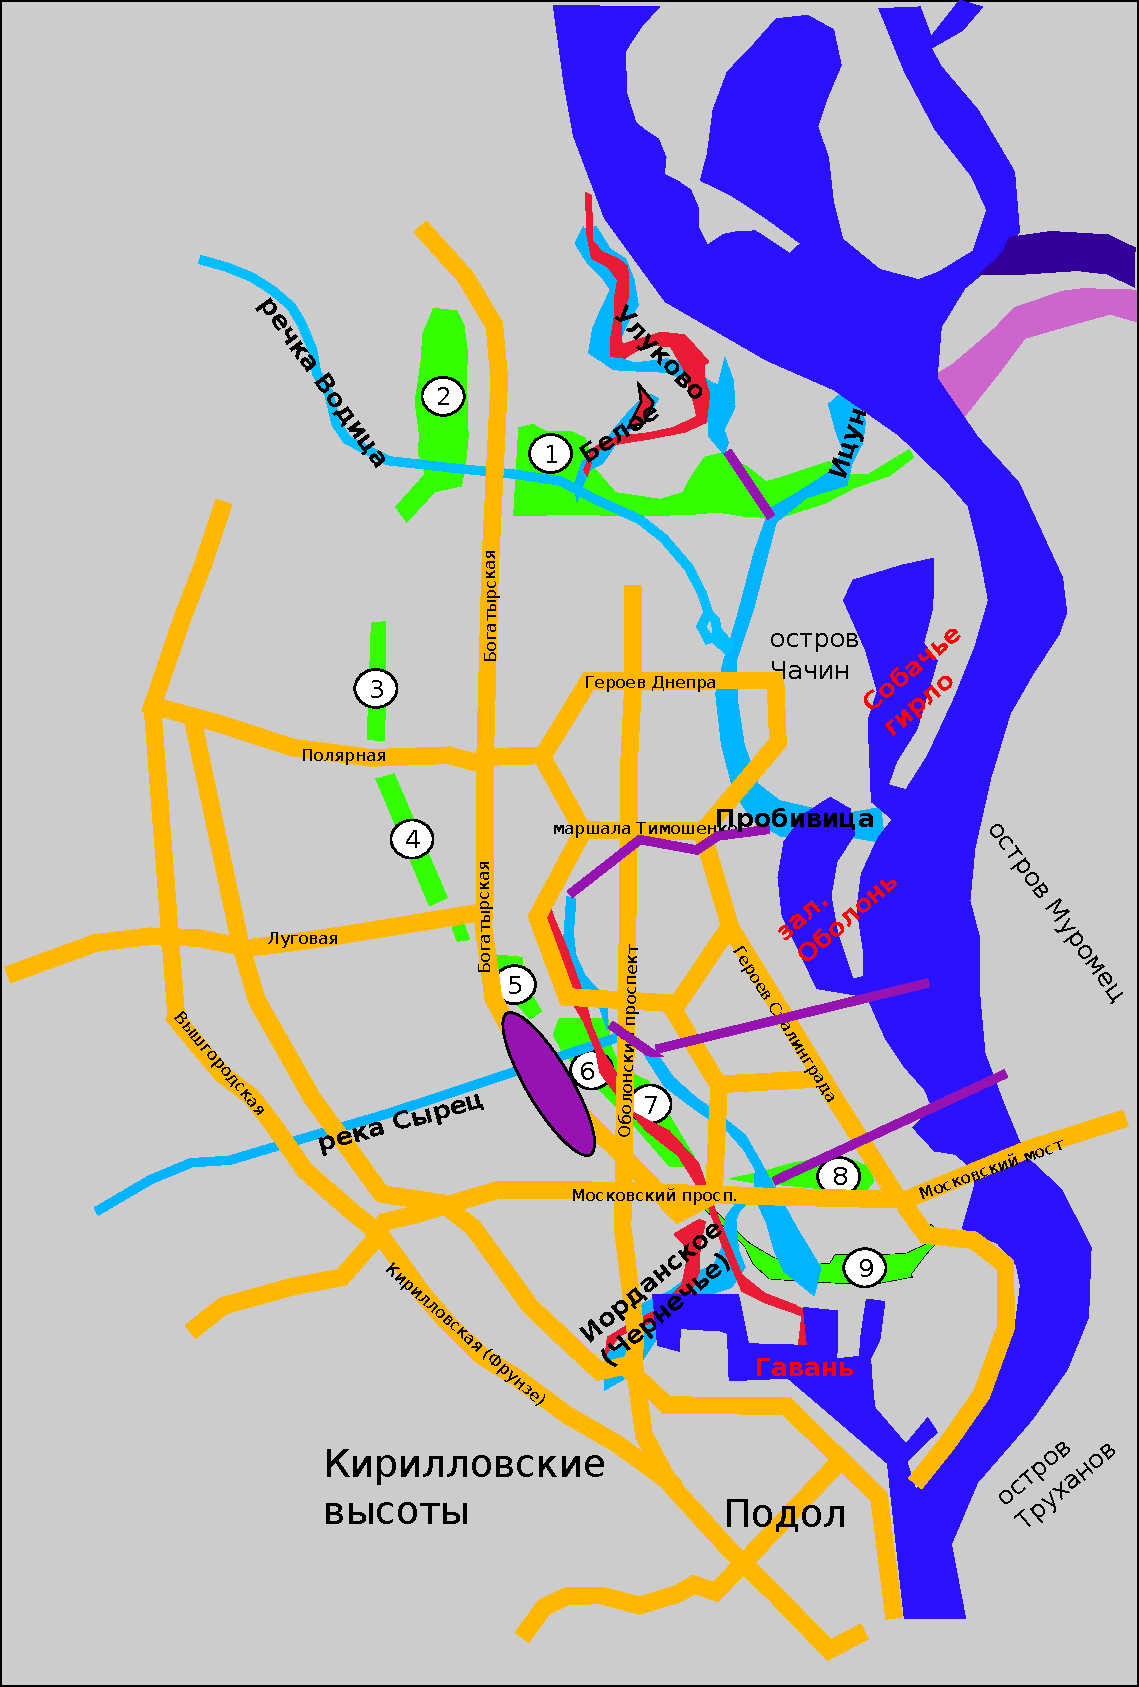
\includegraphics[width=\linewidth]{chast-colebanie-osnov/pochayna/posh2.pdf}
\end{center}
\vspace*{\fill}
\newpage

Мы всё разберем подробно, однако сначала – легенда карты.

Синим цветом обозначено русло Днепра на 2016 год (как вы понимаете, время составления моей карты).

Темно-синий цвет – устье Десны на 2016 год.

Фиолетовое русло чуть южнее – устье Десны за середину 19 века.

Голубые русла – части Почайны-1 по карте Шуберта (середина 19 века).

Красные русла – варианты тех же водоемов за 1914 год.

Фиолетовый овал – примерное место исконного «озера Долгого Кирилловского» с плана Ушакова. Затем так стали называть часть русла Почайны-1 до Иорданского озера. Современное Кирилловское – несколько в стороне от обоих Долгих Кирилловских.

Фиолетовые линии – соединяющие части Почайны-1, показаны приблизительно, известные по плану Ушакова и земельным документам.

Салатовые объекты – современные озера и заливы, возникшие по естественным и противоестественным причинам, вот они пронумерованы:

1. Залив Верблюд, на теперешних картах иногда ошибочно отмечен как озеро Луково. Образовался при черпании песка гидронамывом – прожрал пролив Ицун, озерцо Волкушу, обошел с юга озеро Улуково, задел низовье Белого и пересек давнее русло речки Водицы. Современное «Белое» на картах Оболони – остаток русла Почайны. С юга Верблюд поджимают гаражные кооперативы, между ними и берегом – заросшая вербами луговина, на которой, однако, хорошо прослеживается\footnote{Эдак тут 50°31'57"N 30°30'4"E} отрезок русла речки Водицы, давно от нее отрезанный. По сторонам его стоят очень высокие и могучие ивы. На плане это часть Водицы, что, пересекшись с озером Белым, отходит от Верблюда на юго-восток. Сей отрезок давнего русла довольно широк, около 50 метров, но сильно зарос болотной травой.

2. Озеро Министерка (Редькино).

3. Озеро Минское. Находится по месту бывших там в начале 20 века канализационных лугов, куда по трубам сбрасывались нечистоты со всего города, дабы лежать и разлагаться естественным образом.

4. Озеро Луговое. Верхней частью задевает те же луга, основной частью – урочище Рейтарское.

5. Озеро Богатырское.

6. Озеро современное Кирилловское.

7. Озеро современное Иорданское. Лежит восточнее исконного Иорданского. Положением занимает водоем, обозначенный как «оз. Опечень» на карте РККА 1930-х, что находился по ходу русла Почайны именно в то время.

8. Озеро Вербное.

9. Залив Волковата (Волковатый). В него сейчас прямым каналом выводятся воды из озер «системы Опечень». Заросшая зеленью вода, зажатая между промзоной с севера и железной дорогой с юга. Севернее Волковаты в конце 20 века было еще два озера. На их месте в 2016 году – магазин «Метро» и другие супермаркеты.

Почайну-2 я не рисовал из-за нерешенности вопроса. Не вполне уверен и относительно устья Почайны-1, показал его приблизительно.

Почайну-1 можно считать и рукавом Днепра, и отдельной рекой. Когда связь с Днепром прерывалась, она продолжала работать как самостоятельная река, питаемая за счет малых речек правого берега Киева – Водицы, Коноплянки, Сырца, ручьев Кирилловских высот.

Отрезок Почайны в пределах Подола – для меня загадка. 

Максим Берлинский пишет\cite{berl01}:

\begin{quotation}
За городом Киево-Подолом, в расстоянии около полуторы версты по луговой выгонной стороне, называемой оболонью\footnote{Кстати, в польском языке есть слово «блонь» –  луг. Учитывая, что и поляки, и давние киевляне были полянами, слово «оболонь» того же корня или производное.}, протекает ручей, именуемый Почайною, соединяющийся там же с Днепром. [...] Оный ручей составляет только вершину прежней Почайны. В начале еще 10 столетия составляла  она довольно глубокую речку, протекавшую у самого Подола, отделявшись от Днепра длинною узкою косою, и с Днепром возле Хрещатика соединялась. 

Из архивных Киевского магистрата дел известно, что от 1710 до 1712 года, во время Турецкой войны, приходившие из реки Десны от Брянска барки с казенными припасами заводимы бывали на зимовье, для предохранения от льда, в верх оной Почайны, и причаливались к деревянным клетям, сделанным для укрепления берегов; от чего место это и теперь называется притыкою.

Для сокращения пути в объезд оной земляной косы прокопан был при повороте Днепра прямо к притыке канал, куда скоро все течение реки устремилось, и по времени Днепр, так сказать, поглотил сию Почайну, срезав между нею и собою слабую земляную преграду. 

С тех пор Днепр стал протекать у самого Подола и беспрестанным в весеннее наводнение отмыванием его берегов весьма приметно умалил сию часть города, так что до сего времени считают до 300 убылых дворов, а Почайны осталась одна только вершина.
\end{quotation}

Рожденный там же, на Подоле, в доме около Флоровского монастыря, Николай Закревский полагал, что застал остатки этой косы, к его времени превратившейся в «довольно высокий песчаный остров», покрытый лозой. В «Описании Киева»\cite{zakr01} Закревский говорит, что еще в 1814 году остров начинался напротив «бывших кузниц внизу Александровского спуска» (чуть южнее Почтовой площади), а в 1825 – южнее нижнего памятника Владимиру, и:

\begin{quotation}
имел тогда в длину до 60-ти, в ширину не более 7-ми сажень, и отстоял от берега сажень на 40\footnote{1сажень с 1835 года стала равной 2,1336 метра, а ранее была 2,16 метра. Возьмем на вооружение первую меру, современную работе Закревским над «Описанием Киева». 60 сажень это 60*2,1336=128 метров, 7*2,1336 = около 15 метров, 40 сажень * 2.1336 = 85 метров.}.
\end{quotation}

В 1829 году уже и этого островка не осталось.

Островок чуть севернее источника Хрещатика виден на плане Киева 1750 года. На том же плане, в Днепре между Подолом и Трухановым островом – более никаких островов, а «р. Почайна» впадает в Днепр несколько севернее современных улиц Нижний и Верхний вал, и вот там восточнее ее устья – некие острова, вышедшие за пределы карты. На планах спустя сто лет устье Почайны-1 – примерно там же, сдвигаясь то южнее, то севернее. Мы обсудим это позже.

Всё сказанное Берлинским и Закревским вроде бы логично и справедливо. Однако есть другие сведения о притыке. Кстати, «притыку» обычно переводят как «причал», но «притыка» значило в старину и то же, что и «кий» – дубина, палка, колышек. К воткнутой в землю притыке привязывали лодку.

Теперь отстранимся от популярного представления, что Почайна непрерывно протекала вдоль киевских берегов и воспримем сказанное ниже буквально, ибо речь пойдет о Днепре в том месте, где, как полагают, протекала Почайна.

В докладной записке инженер-майора Даниила Дебоскета за 1741 год, в разделе «О Подоле и Нижнем Киеве» отыскалось такое:

\begin{quotation}
1. От Иорданских ворот по Притыке до Днепра, где госпиталь и подле берега до Крещатских ворот палисадник не заставлен, заставить апарель оным полисадником, ров не делать ибо по все годы от вешней воды оный ров засыпается.
\end{quotation}

Аппарель в фортификации это наклонный въезд в окопы, а палисадник или палисад – бревенчатый частокол.

Иорданские ворота, согласно плану Ушакова 1695 года, стояли чуть южнее церкви царя Константина, под северо-восточным склоном Щекавицы. Крещатские ворота, по тому же плану – несколько юго-восточней нынешней Почтовой площади. От Иорданских ворот, мимо еще одних, Воскресенских – на северо-восток к Днепру проходила деревянная ограда Подола, вдоль которой была пущена речка Глубочица (впрочем на плане не показано устье оной). Затем ограда поворачивала на юго-восток.

Как же понимать Дебоскета? Получается, Притыка – нечто, продолжающееся от Иорданских ворот и до Днепра. Но у того же Дебоскета на плане 1753 года низовье Почайны-1 подписано «река прытыка». «Притыки» в летописях нет. Быть может, так в 18 веке обозначали обходное русло Глубочицы, либо ограждение, либо всё вместе, или же просто тамошнюю местность? В одном документе за 1745 год упомянута, наряду с пристанью Наводницкой, «Притыцкая пристань». Позже в этой главе я покажу документ, позволяющий впрочем отождествить Притыку с давним руслом Глубочицы.

Но почему Дебоскет пишет про Днепр? Разве не протягивалась тогда Почайна вдоль Подола и южнее оного?
 
План Ушакова 1695 – самая ранняя подробная карта Киева. На ней нет притыки, зато есть кое-что любопытное и противоречащее традиционному толкованию слов Берлинского и Закревского. Почайна-1 (обозначенная как «Почана») чуть южнее Иорданской церкви впадает в Днепр. А еще южнее, вдоль Подола, ближайший к правому берегу рукав Днепра подписан – «Почана». Её-то я и называю Почайной-2. 

На плане Ушакова, между Подолом же и Трухановым островом в широкой реке – четыре длинных острова, по двум идет дорога на левый берег Днепра через деревянный мост, брод и снова деревянный мост между островами. Дорога подписана: «Дорога из Духовских ворот\footnote{Духовские ворота были в деревянной ограде Подола (в сторону реки), близ церкви Святого Духа, что лежала на север от церкви Бориса и Глеба.} через Почаевский мост».

А как же мимо Подола проплывали суда? Под мостами не могли, мосты нарисованы низкие, на столбиках. Мост на плотах с разводными секциями... Или суда двигались в обход Чертороем? Но через него тоже должен был существовать переезд с бродом или мостом. Но представление о судоходности рек в старину было иным. Тяжелое судно давало осадку ну метр-полтора. У легендарных казацких чаек осадка до 60 сантиметров, а у струг – до метра. Давний корабль мог проплыть там же, где человек переправлялся бродом.

«Почана» на отрезке Почайны-2 продолжалась южнее Подола и смыкалась с Днепром чуть ниже Крещатого яра. Какую же косу между Почайной и Днепром разрыли? В 1695 году в реке напротив Подола нет никакой косы от русла Почайны-1. Есть длинные острова на «Почане», но это уже Почайна-2 возле Подола, в то время – определенно рукав Днепра. Если протоки между берегом Подола и этими островами использовались для прикола судов, то согласно плану Ушакова, этому не было препятствий. Острова же по виду сами производят впечатление длиннющей косы, в которой прорыто несколько проливов, но впечатление может быть обманчиво.

Ежели эти острова – часть былой косы, то разрытие оной следует отнести ко времени, предшествующему составлению плана, то бишь до 1695 года.

Рассмотрение плана Ушакова в нужном нам районе подбросит больше вопросов, чем ответов. Из-за большой ширины изображения я разбиваю его на два «кадра» – верховья Почайны-1 и остальное. 
\vspace*{\fill}
\begin{center}
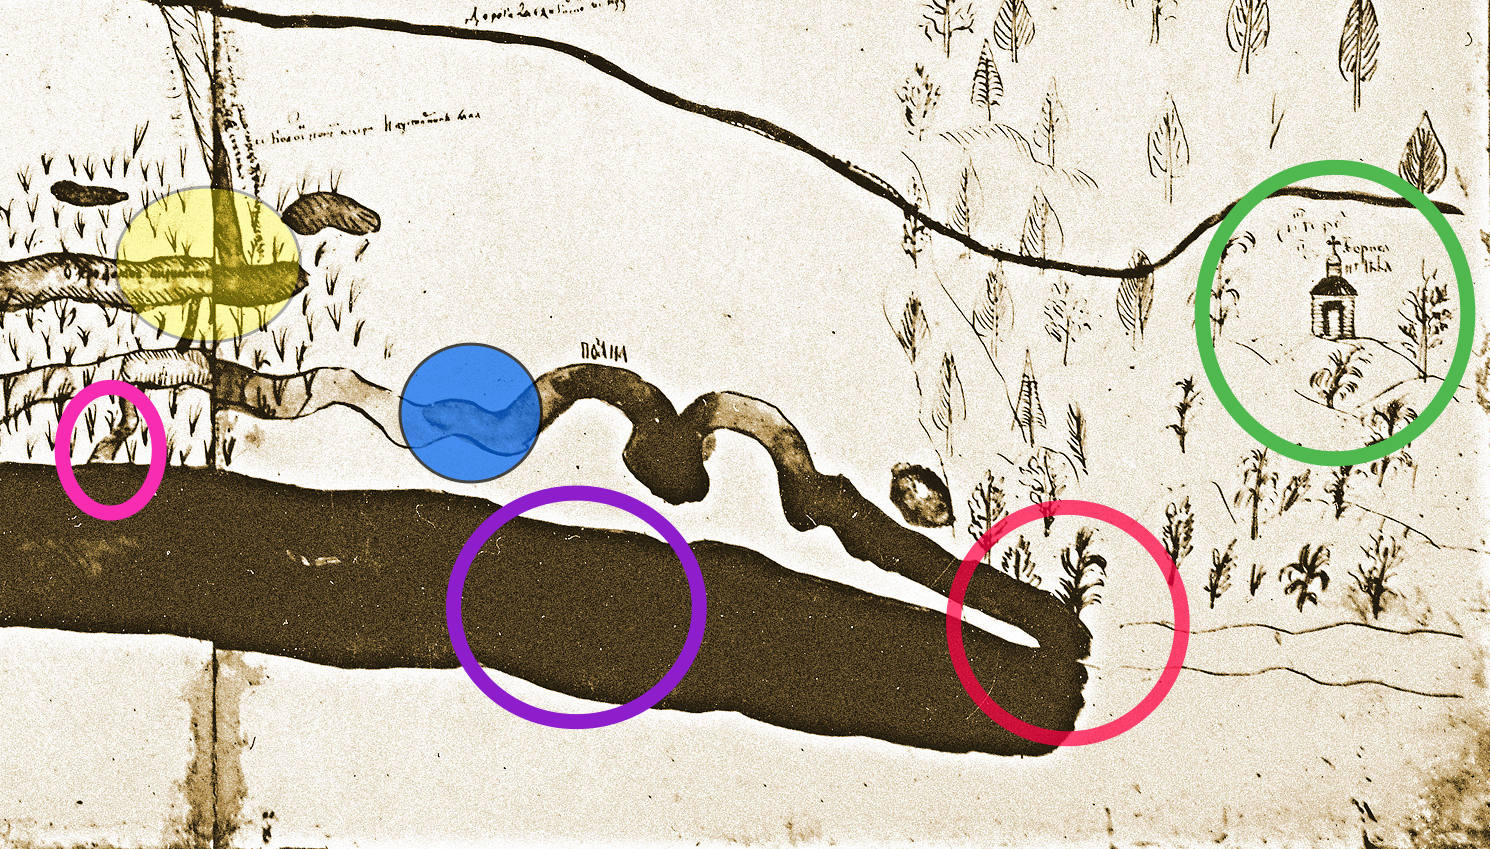
\includegraphics[width=\linewidth]{chast-colebanie-osnov/pochayna/po1695-p2ist.jpg}
\end{center}
\vspace*{\fill}
\newpage

Фиолетовый кружок – Днепр.

Синий – русло Почайны-1.

Желтый – место впадения речки Сырец в «озеро Долгое Кирилловское». Это не современное Кирилловское. Как видим, из старого Кирилловского идет канал в Почай\-ну-1. Вокруг изображены кусты или болотная трава.

Розовый – канал из Почайны-1 в Днепр. Я плохо себе представляю, как работала вся эта речная система вживую. Например, вода через этот канал вытекала в Днепр или наоборот, из Днепра попадала в Почайну?

Зеленый – церковь святых Бориса и Глеба, в Вышгороде, на нынешней северной его окраине, между Вышгородом и Межигорьем, на улице Калнишевского. Поскольку во время составления плана Ушакова Вышгород существовал как-то поболе одной церкви на горе, предположу, что на плане она нужна была как ориентир. Хотя почему бы не написать просто «Вышгород»?

Красный – так изображен исток Почайны-1. Толковать точно не берусь. Поверхностно оцениваю картинку так – южнее Вышгорода от Днепра отделяется рукав. Это-то отделение и есть исток Почайны-1, согласно плану. Может это и есть протока Ицун.

Тут вопрос о направлении течения. Привычно думать, что из Днепра отделялся рукав на юг, там в него впадали притоки вроде Сырца, и всё это неслось к Подолу. Но что если воды Сырца после вливания в Почайну-1 текли на север? Течет же на север относительно близлежащий Ирпень. Да, сейчас вода в озерах системы Опечень движется с севера на юг. Но справедливо ли это для давней Почайны на каком-то ее отрезке? А может, направление течения в некое время изменилось?

Возле истока Почайны-1 видны – озеро, хвойно-лист\-венный лес (план Ушакова радует глаз изображениями разных видов деревьев), направо отделяется незакрашенное русло шириной с ту же Почайну-1, а сверху картинки, по краю леса, сходит расширяющаяся к берегу полоса.

Теперь глянем на участок плана южнее, в сторону Киева. Самое широкое темное русло справа – Днепр.

\begin{center}
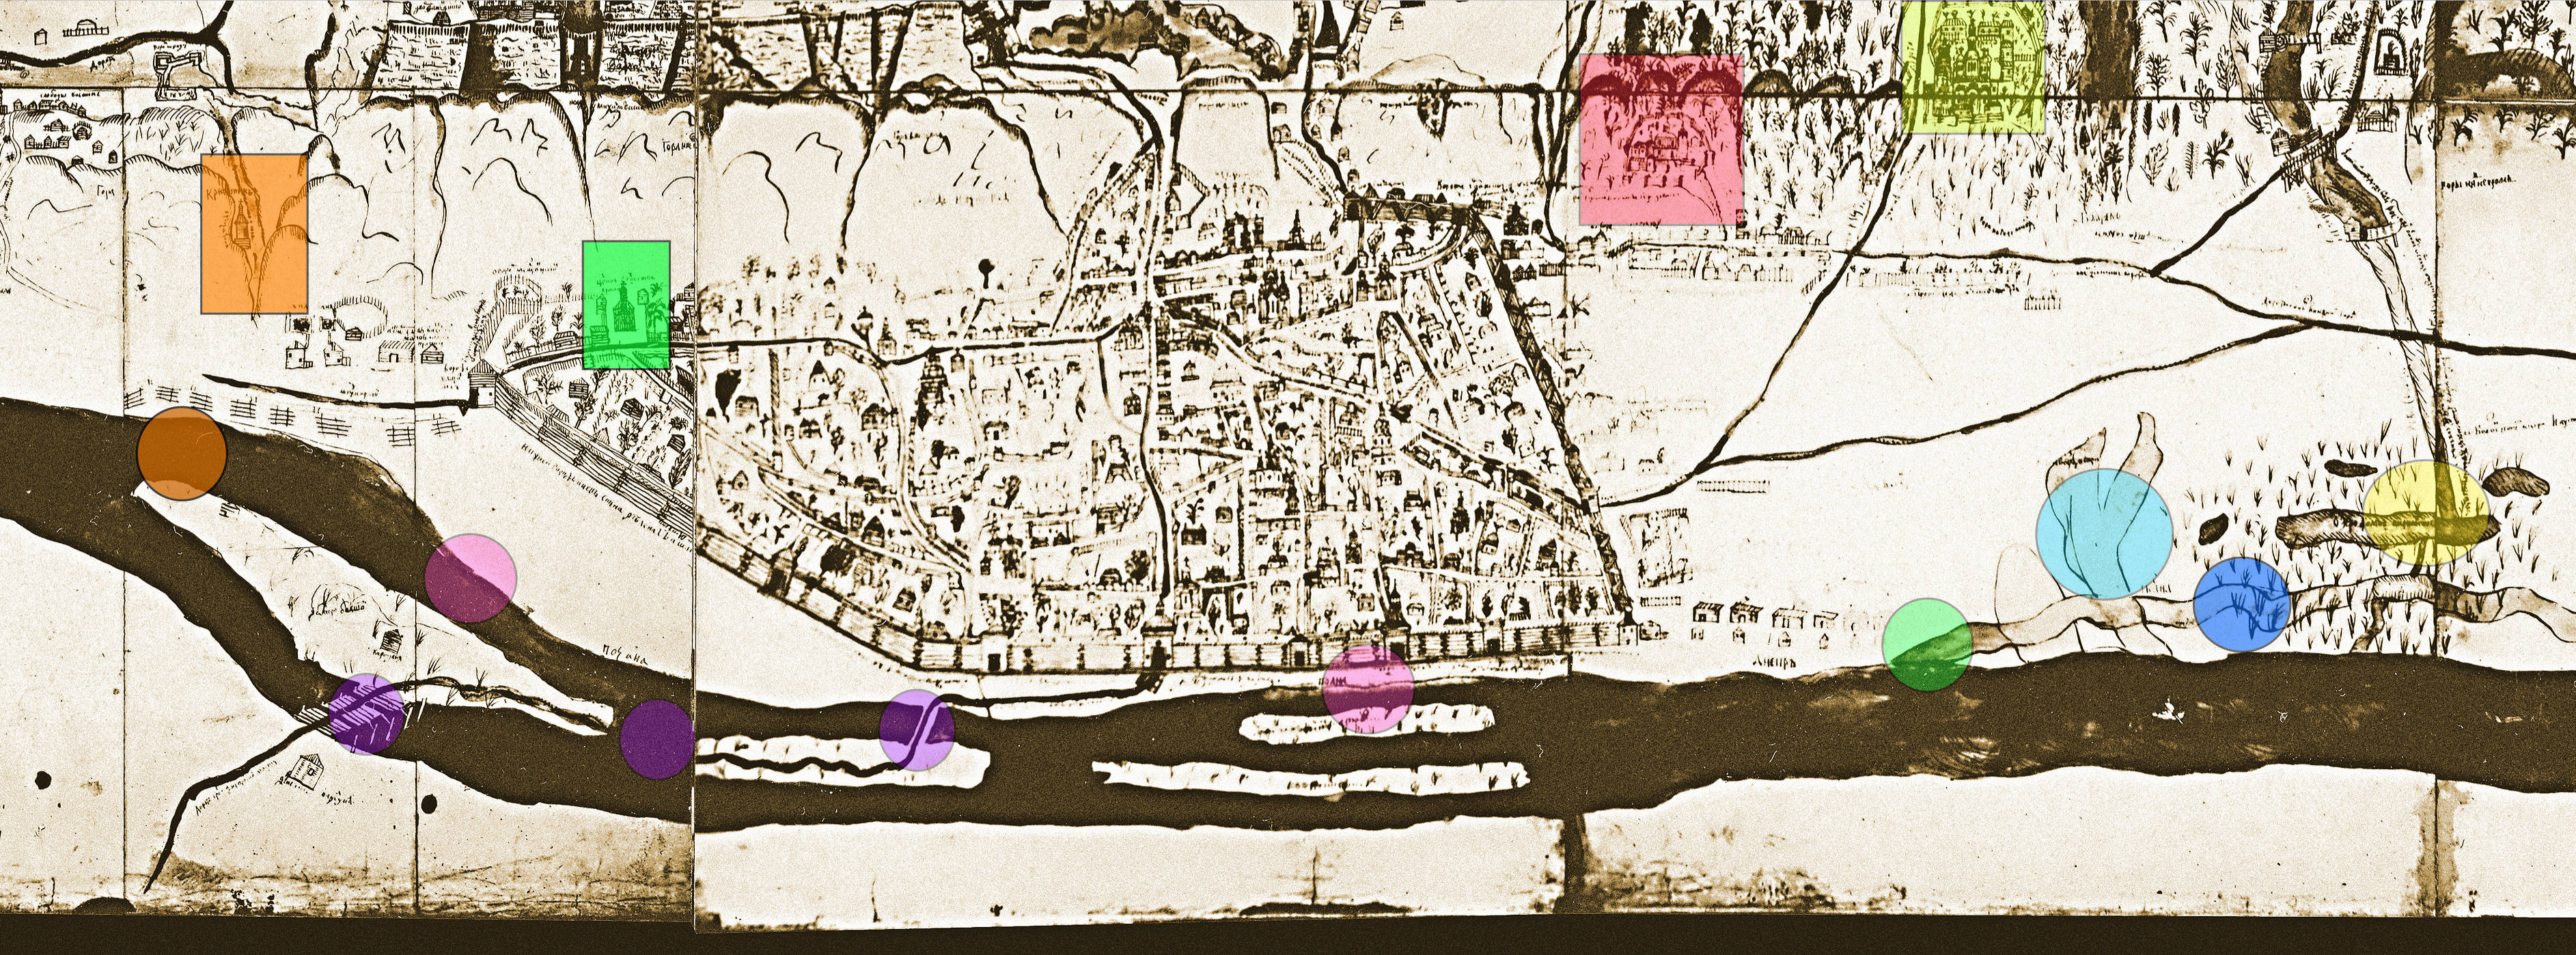
\includegraphics[width=\linewidth]{chast-colebanie-osnov/pochayna/po1695.jpg}
\end{center}

О кружочках.

Синий – русло Почайны-1, чтоб вы сразу поняли, где оно.

Желтый – озеро Кирилловское Долгое. Его сверху вниз (примерно с запада на восток) пересекает русло речки Сырец.

Голубой – озеро Иорданское (старое, не современный самозванец). От его пересечения с Почайной-1, к Днепру идет протока.

Зеленый – устье Почайны-1. Как видим, оно впадает в Днепр. 

Фиолетовые кружки – это места переправы через Почайну-2 от Подола на левый берег Днепра.

Розовые – Почайна-2. На плане Ушакова там написано: «Почана».

Оранжевый – устье Почайны-2, слияние с Днепром.

Теперь о прямоугольниках.

Красный – монастырь Иорданский, примерно где нынче Иорданская церковь.

Желтый – монастырь Кирилловский, там где теперь Кирилловская церковь.

Зеленый – церковь Рождества Христова на Почтовой площади, тоже хороший современный ориентир.

Оранжевый – Хрещатый яр.

Мы видим, что Иорданское (Чернечье) озеро – напротив Кирилловского монастыря. В действительности же оно лежало почти у Иорданской церкви, чуть севернее. Вопрос искажений карты 1695 года, ведь она делалась на глазок, неразрешим. Протяженность Подола с севера на юг, по плану, в два раза превышает расстояние между Иорданским и Кирилловским монастырями. Длина современного Подола (несколько большая, чем в 1695 году), примерно равна расстоянию между упомянутыми монастырями.

Таким образом план Ушакова я могу трактовать лишь следующим образом – объект А следует за объектом Б, между ними объект Ц, и так далее, то бишь план верно отражает взаимосвязь объектов, однако не расстояние между ними.

Мы можем доверять сведениям о Почайне-1 и Почай\-не-2 в том смысле, что два разных русла обозначены на карте одним словом – «Почана». И судить так, что устье Почайны-1 было где-то севернее тогдашнего Подола, а русло Почайны-2 – около его берега. Но где именно было устье Почайны-1, вычислить по плану не получается.

А исток ее – в Днепре. И значит, Почайна-1 это полноценный рукав Днепра. Привлекая данные из других источников, можно предположить, что исток на плане Ушакова это пролив Ицун, известный по старинным документам и прослеживающийся на ряде карт уже как озеро по начало 20 века.

А каким было устье Почайны-1? На плане Ушакова оно широкое, на плане 1750 года тоже. На плане 1786 года видно широкое русло Почайны (треть или четверть Днепра), со стороны Кирилловских высот в него вливается длинное Иорданское-Чернечье озеро, и от места слияния в сторону Днепра, к Подолу, ниточкой вьется ручеек либо канал.

На плане 1843 года ниточка ручейка соединяется уже не с Днепром, но заливом, что начинается напротив Подола около улиц Верхний и Нижний вал, и тянется на северо-запад до уровня перекрестка улицы Нижнеюрковской с Фрунзе. Сравнивая с планом 1786 года можно судить, что этот залив (в 19 и начале 20 веков именуемый Оболонским, а ныне название «залива Оболонь» носит совсем другой водоем) – оторванный рукав Днепра, и что русло Днепра за прошедшие годы сместилось там южнее.

\newpage

\begin{center}
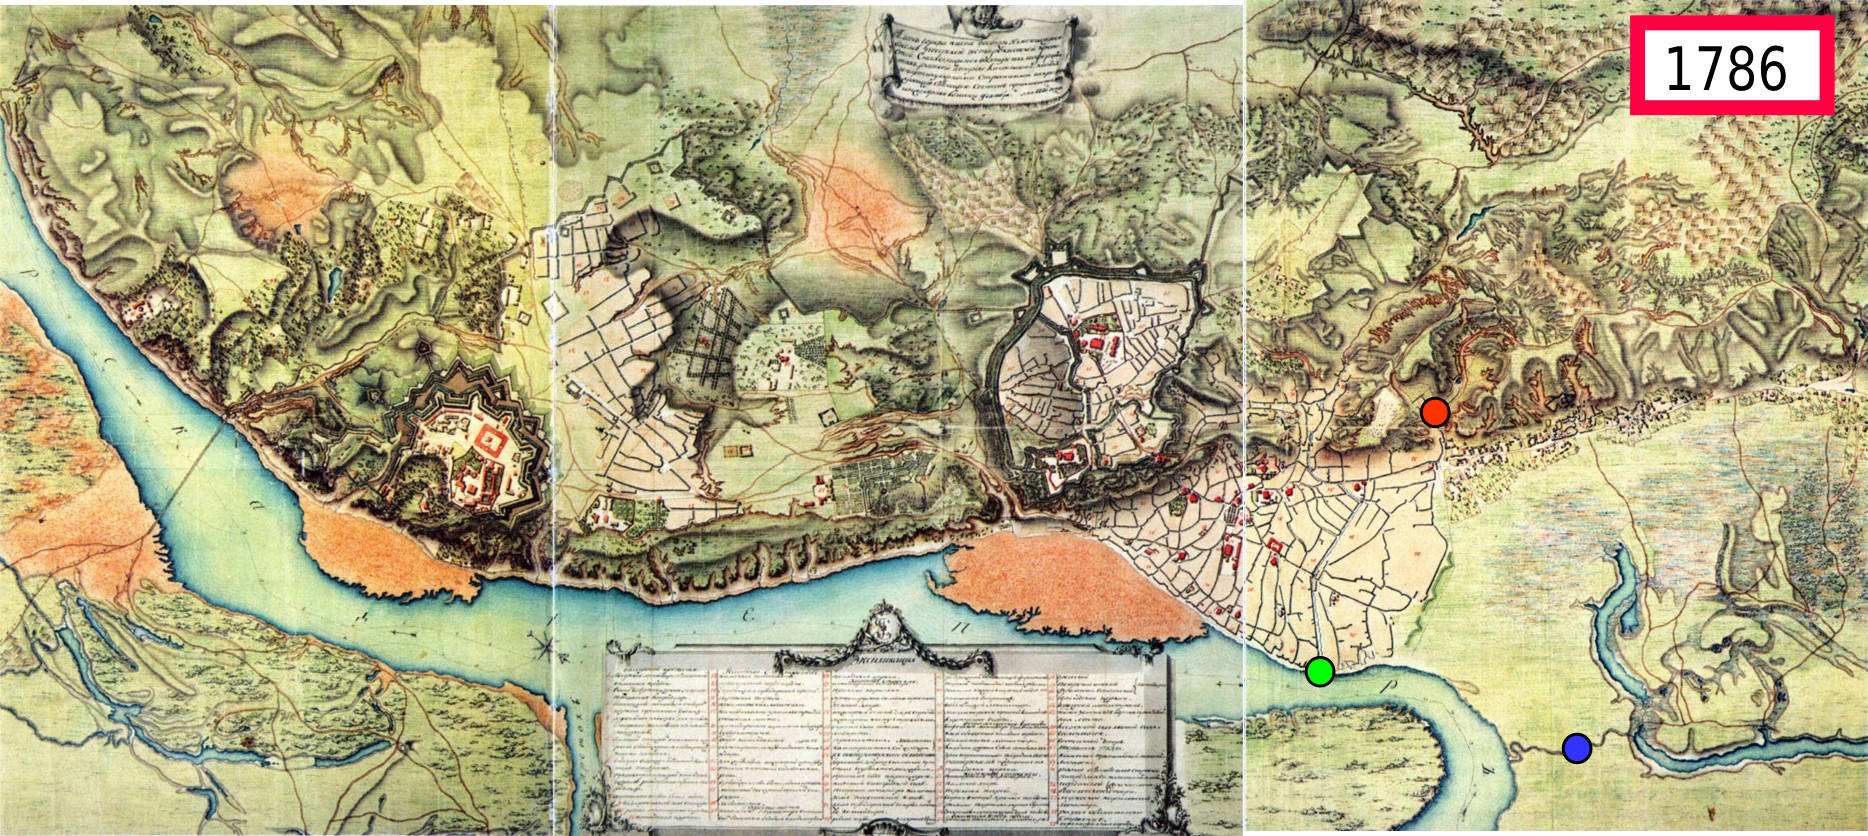
\includegraphics[width=0.92\linewidth]{chast-colebanie-osnov/pochayna/1786-po.jpg}
\end{center}

\begin{center}
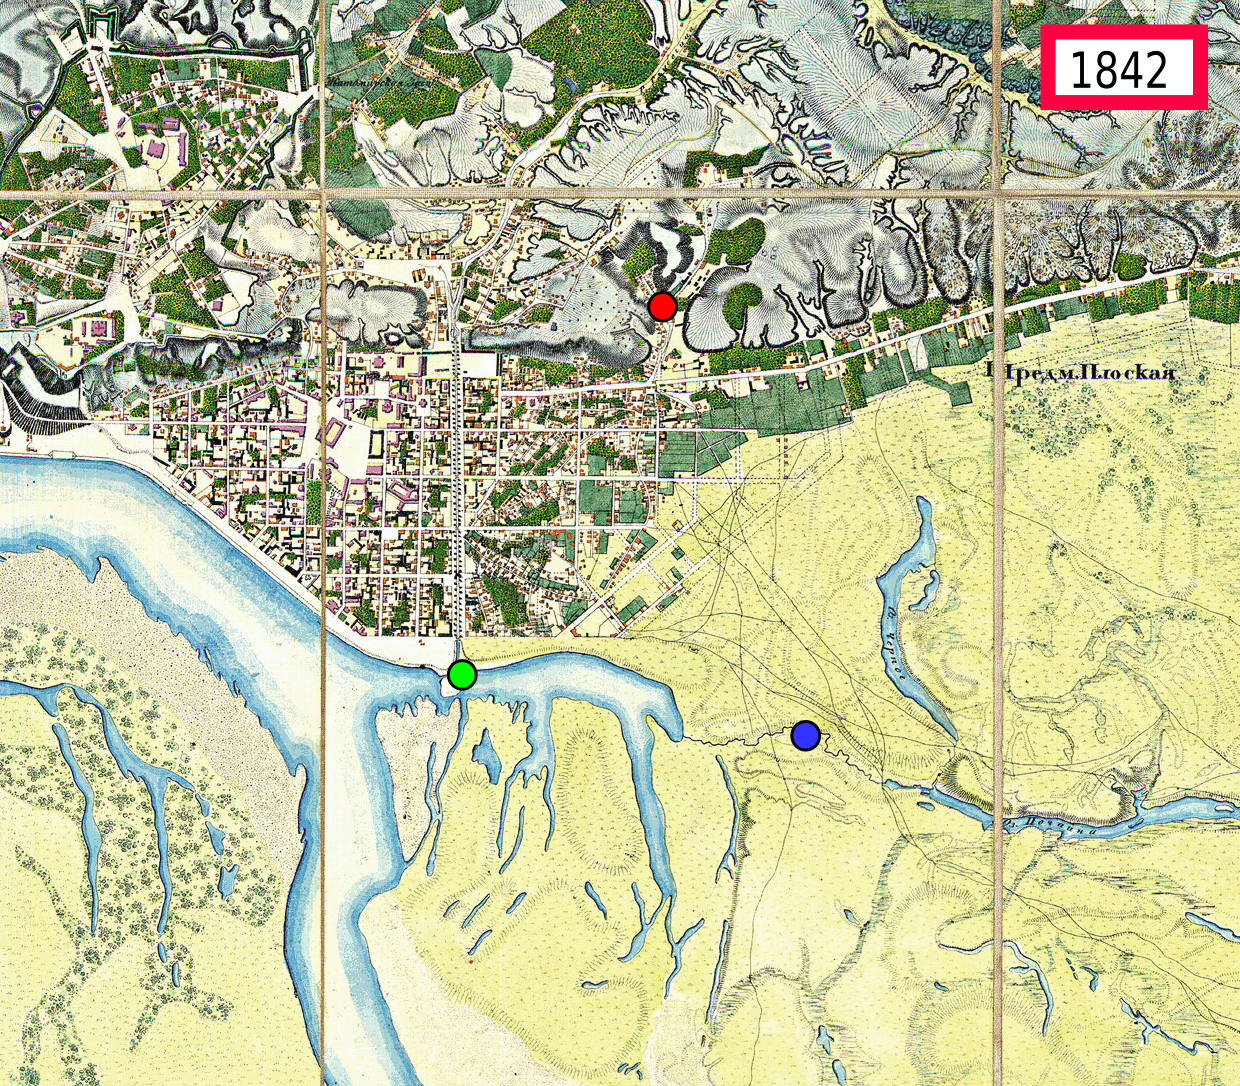
\includegraphics[width=0.92\linewidth]{chast-colebanie-osnov/pochayna/1842-small.jpg}
\end{center}

Красный кружочек – хороший ориентир, «Ерданские рогатки», сейчас это перекресток улицы Нижнеюрковской и Нижнеюрковского переулка. Зеленый кружочек – примерно там сейчас выходят к Днепровской набережной Верхний и Нижний валы. Синий кружочек – «ниточка», идущая к Подолу от места слияния Иорданского озера и русла Почайны-1.
 
Между картами – 56 лет, и как широко за них гульнуло русло Днепра. Что же говорить о временах летописных, о веке княгини Ольги? Девятьсот лет прошло с ее предложения византийскому императору постоять в Почайне!

Далее я перечислю все составляющие Почайны-1 и Почайны-2, поскольку река это ее притоки. Не затрагиваю вопрос водоема Сетомли – на основании летописей вообще нельзя сказать, что это такое.

Двинемся по давней Почайне с севера на юг. Начнем с Почайны-1.

Верховье. Три составляющие, перечисляю с востока на запад: речка Водица, озера Улуково и Белое (смежные), днепровский рукав Ицун.

\textbf{Водица} – речка, давшая название дачному поселку Пуща-Водица. Потерялась где-то во времени, сгинула с современных карт. На трехверстовке Шуберта середины 19 века Водица показана как короткий ручей, что начинается примерно в 1,90 километрах южнее Водогона\footnote{Примерно по координатам 50°32'59"N 30°27'20"E. А Водогон это поселок Днепровской водной станции.}, на восток от 44 и 62 лесных квадратов. Водица огибала там нынешние усадьбы сильных мира сего по восточной их границе, затем по восточной же – дом отдыха «Пуща водица», что ныне на балансе Государственного управления делами. А окончание Водицы показано вроде бы у южного конца хутора Редькина\footnote{\textasciitilde{}50°32'14"N 30°28'27"E} возле нынешнего озера Министерки, но из соображения, что русло на плане Шуберта перекрыто надписями, предположу, что оно продолжалось на восток к озеру Белому, мимо него, а потом впадало в ту же Почайну-1 на юго-восток от Белого, ибо на плане видно, как от Белого к Почайне-1 идет какой-то ручей и впадает в нее восточнее станции метро «Героев Днепра», эдак около домов 57, 56, 63 на одноименной улице\footnote{50°31'26"N 30°30'27"E}.

Поскольку возле южного берега залива Верблюд я видел русло\footnote{Южнее и севернее условной линии между 50°31'57"N 30°29'57"E и 50°31'47"N  30°30'21"E.} по месту и направлению «шубертовской» Водицы, считаю свою догадку верной.

Я не добрался еще к самой Министерке и не осмотрел местность, и у меня нет каких-либо проверенных сведений, жива ли речка Водица, высохла ли, протекает ли в коллекторе или естественном русле. На картах она давно не обозначается.

\textbf{Озеро Министерка}. На месте этого здоровенного водоема раньше, по народной молве, было небольшое озерцо, хотя карты первой половины 20 века показывают там луга на восточном берегу хутора Редьки (в прошлом Редькино, Редькин). Поначалу в самом деле хутор, теперь это жилой массив «хутор Редьки», где кроме новых теремов, еще в 2016 год стоит частный домик 1949 года постройки. 

%До 2002 года на хуторе дислоцировалась 37 отдельная бригада связи. 

Привычное озеро Министерка возникает уже на советских картах, эдак с 1980-х. Водоем вытянут с севера на юг, с явным поворотом в нижней части в сторону озера, следующего к югу по цепи – Минского. Современный размер (полтора километра на почти 400 метров) и глубина (9-14 метров) Министерки указывают, вероятно, на разрытие его при строительстве жилмассивов Оболони в 1970-х и позже ради добычи песка для гидронамыва.

Бытующее в народе название возникло, когда на части нынешнего западного берега появился дом отдыха или санаторий Совмина. По одним сведениям, правительственный санаторий появился тут в 1936 году, по другим – в 1960-х. Он и сейчас там, подчиняясь другому ведомству. Целый комплекс зданий в лесу, включая подсобное хозяйство с грядками, свой отгороженный пляж – самый большой на озере. Противоположный берег, за Богатырской улицей, застроен медицинскими учреждениями, а с 2014 года и районом элитного жилья «Итальянский квартал». Там же лежит западный конец залива Верблюд.

У купавшихся в Министерке в девяностые «немного желтела кожа и отчетливо желтели ногти» – полагали, что в воде много йода.

Вода в Министерке вроде чистая. Как и многие водоемы Киева, Министерка облюбована браконьерами. По данным ныряльщиков, дно неровное – бугры, какие-то проходы, заиленные ямы.

Полагаю, что если по течению речки Водицы находилось «озерцо», позже расширенное в Министерку, то это был хуторской пруд.

\textbf{Улуково}. К востоку от Министерки, через ревущую транспортом улицу Богатырскую, что является магистралью на Вышгород, лежит залив Верблюд. Его окрестности прежде слыли урочищем Влуково или Улуково. Значит «у лук». Лука – поворот реки, загиб. В урочище лежало два крупных озера. Большее называлось Улуково (Лукомье, Луково, Вовлукомье), меньшее – Белое. На ряде старых карт оба слившихся озера подписаны как «Улитка».

В излучине Улукова находился хутор Никольский (бывший Малый Никольский, ибо в лесу Пущи-Водицы есть просто Никольский). На 2016 год его можно соотнести местностью чуть южнее одной из частей коттеджного комплекса «Итальянский квартал»\footnote{Хутор был примерно здесь – 50°32'18"N 30°30'16"E}.

Улуково озеро огибается с юга заливом Верблюд, который, вгрызаясь в тело покрытого осокорами да травой острова Чачина, пересек залив Ицун, прошел у низовья Улуково, поглотил часть Белого и русла Водицы. В 20 веке обратилась вода в сушу, а суша в воду. Сгинул Ицун, а Днепр в той местности приблизился к правому берегу на половину ширины своей.

От Ицуна и Улукова русло Почайны шло на юг – это место видно на нарисованной мною карте, и примечательно, что часть сего русла ниже развилки, от южного берега Верблюда до гаражных кооперативов, сохранилась по 2016 год\footnote{Начало участка русла: 50°31'60"N  30°30'48"E, конец: 50°31'47"N 30°30'41"E.}. 

Современное Улуково впадает в Верблюд (или наоборот). В 17-18 века Улуково впадало в Почайну. По Шуберту оно уже никуда не впадало. К 1914 году судорожный изгиб Улукова несколько изменился, но озеро сохранило очертания.

К Белому и Улукову, встроенным теперь в северный берег Верблюда, можно добраться, свернув на восток от улицы Богатырской, между Верблюдом и возводимыми с 2014 года на намывных песках домами «Итальянского квартала». Чтобы познать местность, я начал изучение не с главного для меня, а с второстепенного, с южного берега Верблюда.

Если не считать его загиба к Днепру, над другим заливом, Собачьем Гирлом (пишу «гирло», ибо это не «горло»), то берег представляет собой почти прямоугольный, перечерченный грунтовками участок суши длиной около двух километров и шириной почти пятьсот метров. Густая трава, осокоры, несколько по виду заливов, которые на деле – отрезанные, но сохранившиеся участки русел Почайны (западный «залив», точно совпадает с «шубертовским» руслом середины 19 века) и Водицы (а тут небольшое отклонение от «шубертовского» русла).

Ближе к западной части этого прямоугольника, за оградами из жестяных листов и всякого мусора, прячутся огороды.

Всё сказанное здесь справедливо на лето 2016 года – указываю на это в предчувствии дальнейших изменений местности.

На берегу много рыбаков, включая любителей сетки. Есть хилые пляжики. По береговой линии, Верблюд нельзя обойти непрерывно, ибо в юго-западном углу стоит ресторан. Надо выбраться на трассу Богатырской и по ней обойти огражденный участок.

У северного берега Верблюда, между коттеджами «Итальянского квартала» и водой, направо – к востоку – через едко пахнущий верболоз отходит по песку тропа. Она ведет сначала к светленькому малолюдному пляжу, затем конно-спортивной базе, наконец выходит в чисто поле, кажется уже обреченное на застройку.

Восточной стороной оно выходит на широкое, заросшее кувшинками озеро Белое, устьем соединенное с Верблюдом. Белое, как и Улуково, своей длинной формой напоминают части давнего русла равнинной реки, разорванной на части. Ширина Белого – 80 метров в самом широком месте, 40 – в среднем. Длина около 400. С севера и востока озеро огибается, за оградой, на насыпи, стройкой «Итальянского квартала» и уже нанесенной на карты улицей Луковской. «Квартал» отделен от поля рвом, что зарос бурьяном.

Начинаем объезжать будущее жилье. По правую руку – большой мыс между Белым и Верблюдом. За болотцем, где еще лет пять назад был южный «хвост» западного низовья Улукова, сизой зеленью курчавится дубрава.

Это окрестности бывшего хутора Никольского, что прослеживается мною на картах с середины 19 века по сороковые годы 20-го. Он был чуть восточнее, по современному рельефу, близ мыса между Верблюдом и Улуковым. Улуково озеро нижней своей частью похоже на букву «П». Низом правой ножки, прежде оканчивающейся в суше, ныне оно соединено с Верблюдом. А у низа левой ножки лежал хутор\footnote{50°32'20"N 30°30'11"E}. Где-то поблизости вроде бы сохранились остатки водяной мельницы\footnote{50°32'19"N 30°30'9"E}, однако я их не отыскал.

Заболотившаяся левая ножка идет от хутора на запад и почти смыкается с озером Белым.

Северная, верхняя палочка «П» – рукотворный канал, на старых картах его нет, заросло кувшинками, дно ровное песчаное, по цвету бурое, можно перейти вброд.

Суша внутри «П» – густотравное поле с загадочными буграми и прямыми рвами, относящимися ко времени вероятно хутора Никольского, а может и более давнему, учитывая находку археологами древнего поселения на противоположном, южном берегу Верблюда. Поле переходит в тенистую дубраву. Судя по толщине стволов, некоторым деревьям более ста лет.

Основная уцелевшая часть низовий Улукова – правая, восточная «ножка». Она соединяется южной стороной с Верблюдом, а верхней – с упомянутым каналом, откуда, из продолжения северной части левой палочки «П» русло идет на север к гати, по которой проложена дорога. За гатью Улуково следует на запад, с юга зажатое «Итальянским кварталом», с севера дачным кооперативом «Чернобылец 2005», огибая оный и сворачивая затем строго на север. К западу от русла, через пустырь, между ним и улицей Богатырской – корпуса двух больниц, кожно-венерологической и детской. В 2015 году там началось строительство еще одной части «Итальянского квартала», а до революции был хутор Михельсона.

\begin{center}
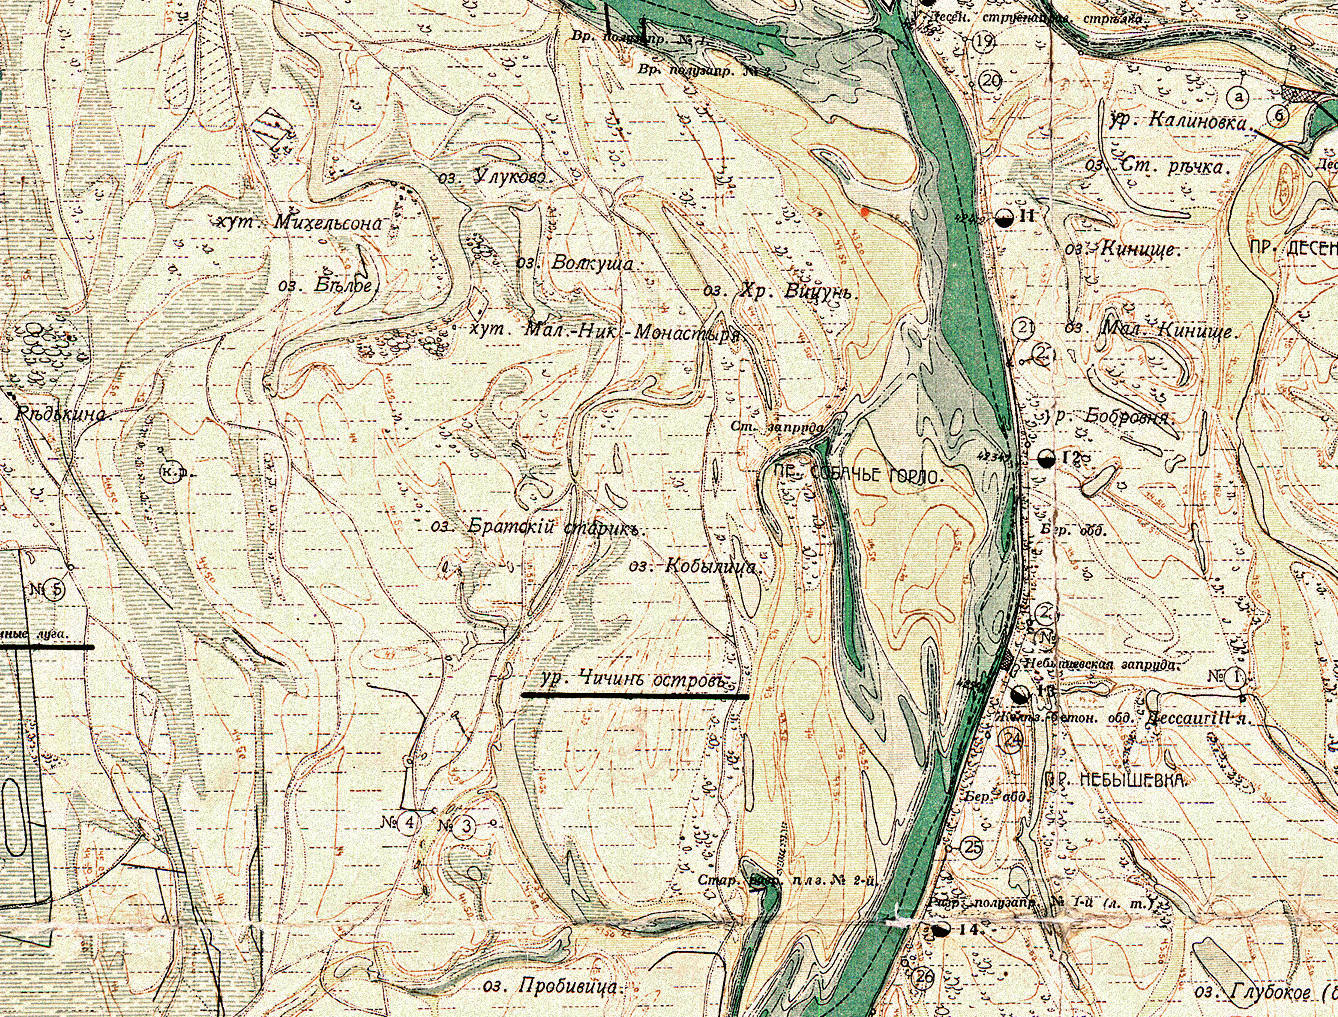
\includegraphics[width=\linewidth]{chast-colebanie-osnov/pochayna/itsunsrc.jpg}

\textit{Кусок плана 1914 года.}
\end{center}

От гати также идет канал на восток к Днепру – это по правую сторону от правой палочки «П». Вопреки некоторым картам 21 века, суша вокруг – не остров Чачин. Остатки земель Чачина лежат южнее, на юго-восточном берегу Верблюда и среди жилых районов между улицами Приречной и Героев Сталинграда.

Какое отношение Почайна-1 имеет к Улуково и Белому? Там был один из ее истоков. 

Изучим выдержки из протокола действий межевой комиссии, назначенной для решения спора о границах между Межигорским монастырем и киевскими мещанами, за 10 октября 1713 года\cite{sbornikmat}. Он написан на «мове роськой», про которую я рассказывал в главе «А так говорят грамоты».

В те времена, для указаний границ землевладений, использовались не карты, но описания. Область определялась как замкнутая совокупность точек-урочищ. От Высокого дуба до Малой речки, Малой речкой до Кривых верб, теми вербами до Черного кургана, а от кургана полем опять к Высокому дубу.

Существовали документы, где были записаны границы. В случае возникновения земельных споров создавались комиссии, изучавшие дело и выходившие на местность, где местные жители, причем старожилы, давали показания, где какое урочище находится. На основании документов, показаний и разбора местности власти должны были принимать решение.

В документах упоминается множество урочищ, давно забытых, чье местоположение восстановить нельзя. Однако некоторых – можно попробовать. И это даст зацепку для дальнейших рассуждений.

Займемся Кривой Почайной.

В упомянутом протоколе действий межевой комиссии сказано, что члены комиссии:

\begin{quotation}
ведены былисмо з Киевского нижнего города чрез браму Воскресенскую – Оболоньем, чрез кривую Почайну поуз речище, прозываемое Ицун, а верх Ицун поромом перевезшися чрез реку Днепр, пристали до берега в острове меском Осетшина зовемом, близ урочища малого Соплика [...]
\end{quotation}

Верх – это север, низ – юг.

Нижний город означает Подол. Брама Воскресенская – Воскресенские ворота в северо-восточной деревянной стене Подола. Ворота назывались так от одноименной церкви (стояла на углу Спасской и Межигорской, исчезла в 1930-е), ибо от центра Подола мимо этой церкви к воротам вела широкая улица.

Выйдя из брамы, комиссия попала на Оболонье, шла по нему, и далее перейдя «чрез кривую Почайну» –  мимо речища (бывшего рукава реки) Ицуна добралась до Днепра, села на паром и переправилась на другой берег к городскому («мескому») острову Осетщине (близ нынешнего устья Десны).

На карте Ушакова 1695 года видно, что дорога из Воскресенских ворот идет по равнине Оболони эдак на север, между Кирилловскими высотами и Почайной-1. За перекрестком с дорогой от Кирилловского монастыря, первая дорога начинает неуклонно сближаться с линией возвышенности, вдоль которой уже тогда от Подола до Сырца лежали прообразы улиц Кирилловской (Фрунзе) и Вышгородской – по сути составные части одного пути. 

Южнее русла Сырца, «наша» дорога вливалась таки в эту старинную Кирилловскую, а уже та пересекала Сырец и следовала в направлении Вышгорода, между горами по левую руку, и равниной с Почайной по правую. Каких-либо надписей про «Кривую Почайну», «Ицун» на имеющихся у меня сканах и копиях плана Ушакова я не вижу.

Соотнесем эти сведения с протоколом комиссии. 

Сырец на плане Ушакова впадает сначала в озеро Долгое Кирилловское, а оттуда канальчик идет в Почайну. Это происходит, по плану и природе, не на широте устья Десны, но много южнее.

Из протокола мы знаем, что, дабы добраться к Ицуну с его паромной переправой (сие широта устья Десны), комиссия в каком-то месте пересекла Почайну Кривую.

Поскольку Ицун лежит севернее Сырца, значит, Кривую Почайну перешли на отрезке пространства между Сырцом и устьем Десны.

На широте Ицуна лежали озера Улуково и Белое. Южнее их, по плану Шуберта, смыкалась с Почайной-1 и речка Водица. Отсекаем – где в тех широтах могла быть Почайна-1 вообще? Западным пределом положим речку Водицу. Северным – упомянутые озера. Восточным – остров Чачин и Днепр. Северо-восточным – Ицун. 

То же самое справедливо для Почайны Кривой – ее верховье не может быть севернее Водицы, Белого, Улуково и Вицуна, если только не пытаться уместить натужно Почайну Кривую между Улуковым и Ицуном.

Значит, Почайна Кривая это по крайней мере название верховья Почайны-1. Забегая вперед доводов, можно предположить, что Почайна Кривая, по руслам, это буква V, образуемая смычкой продолжения на юг Ицуна и низовьем Водицы – смотрите мою карту южнее Верблюда.

А по плану Ушакова видно, что Почайна-1 отделяется от Днепра ниже Вышгорода. И больше до Сырца никакого пролива из Днепра к Почайне-1 не показано. Остается предположить, что днепровский исток Почайны-1 на плане – это Ицун.

Что еще говорят документы о Кривой Почайне? Насколько подтвердятся логические размышления?

В том же протоколе содержатся показания свидетелей со стороны Межигорского монастыря, где дается словесное описание Кривой Почайны. Разные старожилы говорят разное, пользуясь привычными им обозначениями.% Как например жители Зверинца по улице Бастионной или Катерины Билокур считают свой район Печерском, а жители Цитадельной считают Печерском свой район.

Что же поведали комиссии свидетели?

\begin{quotation}
Первый Петро Савенко, житель вышьгородский, ставши очевисто, а приведши нас на границу сознал под совестию души своей: что Почайна кривая граничит от Вышгорода, взявши по едной стороне тоей Почайны, кгрунт (мовить\footnote{Прямая цитата свидетеля в протоколе.}) вышгородский, а по другой стороне той же Почайны Киевских жителей земля лежить, а тая Почайна кривая (мовить) початок свой имеет в Олсове, з Белого озера и з Авлукова, упадает в озеро Василковское.
\end{quotation}

Отсюда можно заключить, что если смотреть на Почайну Кривую от Вышгорода, то по одну сторону Почайны грунт (землевладение) относится к Вышгороду, по другую – к Киеву. Почайна Кривая служит границей земель.

Почайна Кривая начинается, согласно Петру Савенко, в урочище Олсове, из Белого озера и с Авлукова. Трудно в «Авлукове» не узнать Улуково! 

Но что за озеро Василковское, куда впадает Почайна кривая?

В середине 17 века где-то возле Сырца был бор (сосновый лес), а за ним – «грунт», поле Васильевской церкви (подольской, что примыкала к северо-западу Флоровского монастыря, или одноименной церкви верхнего города).

Приведу описание границ угодий церквей Воздвиженской и Трехсвятительской, из Грамоты царей Иоанна и Петра Алексеевичей, подтверждающей Киево-Братскому монастырю права на земли и угодья, 11 января 1694 года:

\begin{quotation}
[...] озеро Василевское у Чорторый за Днепром с сеножатьми, промеж Чорторый речки, и промеж тогож озера Васильевского во Влуково урочище, три озера з зарожками, крыницами: одно великое прозвищем Три-тони, сверху выше Котельни криницы Воздвиженской, почав от лоз верхних, даже на низ жерелом в другое озеро, Воздвиженское прозванием, Долгое и Уское, которое взялось от Киева и кончится в озеро Три-тони.

Третье из того ж великого озера Три-тони, жерелом пошло промеж лоз и промеж черету к дороге Вышгородской, там же промеж тех озер и лоз сеножати Воздвиженские, сверху вниз с конца в конец.
\end{quotation}

Уцепимся за «озеро Василевское у Чорторый за Днепром с сеножатьми, промеж Чорторый речки». Есть урочище Черторый и одноименная речка. А урочище это прыгает с места на место. Скажем, на карте 1914 года так подписана местность южнее нынешнего Московского моста, а уже в 1991 году – севернее оного.

По тексту неясно мне, то ли граница земли шла на другой берег Днепра к урочищу Черторые либо одноименной реке, то ли имеется в виду озеро не примыкающее к Черторые (урочищу либо водоему) непосредственно, однако лежащее с ней на одной широте.

Упоминание «озера Василевского близ Чортории» в универсале гетмана Даниила Апостола в подтверждение Киево-Братскому монастырю прав на владения селами и угодьями, от 13 января 1729 года, кажется, говорит в пользу первого предположения.

Однако что находится у нас на широте Московского моста, несколько южнее его? Устье Почайны-1. Слова старожила, что Почайна Кривая «упадает в озеро Василковское» приобретают некий смысл. Быть может, близость Васильевского озера к Черторые следует трактовать как близость по широте, однако не нахождение Черторыи и Васильевского на одном берегу? И озеро следует искать на Оболони, южнее Московского проспекта?

На карте 1750 года есть еще левобережное озеро Васильевское, несколько севернее Лавры. От Никольской слободки (район станции метро Левобережная) оно впадало в речку Черторыю либо вытекало из нее. Но это далеко. «Наше» Васильевское я нашел гораздо ближе.

В мировом соглашении между  Кирилловским монастырем и Киевским магистратом по поводу спорных земель, 1767 года сказано:

\begin{quotation}
Что ж принадлежит до сеножати Ковальской, она ж и Римарская\footnote{Коваль – кузнец, римарь – шорник, изготовитель лошадиной упряжи.}, которая под владением Киево-Кириловского монастыря состояла, по окружности учиненного дьяком Алфериевым дукта\footnote{Дукт – линия размежевания.}, то и той Римарской сеножати сделал (неразборчиво) же ограничение по нижеписанному, а имянно:

Начав с первого места от самой вершины Долгого Кириловского, оно ж и Закотнее, озера (неразборчиво) смуговиною поуз сеножати в леву сторону сначала мещанина киевского Романа Чишанича Власенка, а далее умершего обозного полкового Василия Ви(?)евского, да сеножати попа царя-константиновской церкви Дионисия Силванского до круши(???)его Куста и до старого Алфериевского копца\footnote{Копец – столбик или яма для обозначения очередной точки границы.}, зделанного ямою при дорозе идучой, а тою дорогою поуз сеножати в леву сторону того ж попа царя-константиновской церкви до Рудки грузкой, через которую пребить трудно, а перешедши тую Рудку, взять в леву сторону, тею Рудкою смуговиною, до дороги последней от Днепра, которую теперь взять з Вижгорода до Киева, и тою дорогою, поуз сенокос Киево-Михайловского монастыря, до копця старинного Алфериевского, а от того копця просто в смуговину, тою ж смуговиною на рог бугра, а оттоль поуз озеро, называемое Михайловское, оно ж и Василиевское, чрез болото отколь начинается по леву сторону сенокос монастыря Киево-Кириловского, а по праву сторону сеножать Римарская, от того ж болота до ковтобини же простуючи до озера, а перешедши тое озеро на криницу, которая и по крепостям Римарским значится, оставля тую криницу в стороне Римарской [...]
\end{quotation}

Несмотря на появление неведомой нам смуговины Рудки и других канувших в небытие урочищ, мы узнали, что озеро Васильевское называлось еще Михайловским (вероятно, от Киево-Михайловского монастыря), рядом с ним было болото, а добраться туда можно было, так или иначе, от дороги из Киева на Вышгород. Кроме того, Римарская сеножать именовалась Ковальской, а она, как мы увидим несколько позже, лежала не так уж далеко от Иорданского озера.

Любопытно также подробное описание озера Три-тони в урочище Влукове (легко угадывается Улуково). Для расстановки сил процитирую еще из грамоты от 11 января 1694: «озера прозываемые: Три тони, Долгое и Узкое, и озеро Василевское».

Три озера. Более чем вероятно, что в других документах они проходят под другими именами. Большое озеро Три-тони в урочище Влукове – скорее всего Улуково и Белое, слившиеся.

Долгое и Узкое, оно же Воздвиженское – «взялось от Киева и кончится в озеро Три-тони». Значит, длинное и узкое по виду. «От Киева» – протянулось от широты Киева или со стороны Киева? И до Трех-Тоней. Если от широты, то пожалуй, это главное русло Почайны-1! На плане 1752 года часть этой роли отведена озеру Долгому Кирилловскому (лежащему восточнее одноименного с плана Ушакова).

При этом в документе не упомянута Почайна Кривая, а просто Почайна упомянута кратко, что дано право (владение землей) на «оболонь под Киевом над Почайною меж полями и сеножатьми Преворской и Лесковскою будучею, а другую Свершковскую».

Однако мы узнали, что озеро Васильевское носит и другое имя, Михайловское. Последнее показано на карте 1752 года, к которой мы еще обратимся не раз. Таки на Оболони, между Почайной и Днепром, на широте между Кирилловским и Иорданским монастырями. Стало быть, в протоколе 1713 года свидетель показал, что Почайна Кривая лежала от Улуково и до широты между Кирилловским и Иорданским монастырями. Отмечу, что на карте 1752 года положение Почайны Кривой совершенно отлично от словесных описаний в протоколе комиссии, однако мы обсудим это противоречие позже.
 
Вернемся к протоколу и послушаем другого свидетеля-старожила. Он говорит, от каких и до каких урочищ идет Кривая Почайна:

\begin{quotation}
Вторый Иаким Туз, вышгородский житель, кгды был призванный и допрошуван, если бы подлинно ведал отколь взялася кривая Почайна, и на якие идет урочища, теды сознал под совестию: же Почайна кривая взялася (мовить) з Днепра, а идет за сажение\footnote{Посаженные.} вербки, а одтоль з саженных вербок упадает у Тушанку, з Тушанки в долину Старцеву, з долины Старцевой в реку Горенку.
\end{quotation}

По мнению Туза, Кривая Почайна начинается из Днепра, да идет за высаженные вербы, а оттуда к Тушанке. 

\newpage

\begin{center}
\includegraphics[width=0.98\linewidth]{chast-colebanie-osnov/pochayna/\myimgprefix IMG_20160621_140248.jpg}

\textit{Залив Верблюд, вид с южного берега.}
\end{center}

\begin{center}
\includegraphics[width=0.98\linewidth]{chast-colebanie-osnov/pochayna/\myimgprefix IMG_20160621_140528.jpg}

\textit{У южного берега Верблюда, вербы растут вдоль перерубленного, заболоченного русла Водицы.}
\end{center}

\newpage

\begin{center}
\includegraphics[width=\linewidth]{chast-colebanie-osnov/pochayna/\myimgprefix IMG_20160621_144150.jpg}

\textit{Остатки озера Белого.}
\end{center}


\begin{center}
\includegraphics[width=\linewidth]{chast-colebanie-osnov/pochayna/\myimgprefix IMG_20160621_151157.jpg}

\textit{Окрестности Никольского хутора между озерами.}
\end{center}

\newpage

\begin{center}
\includegraphics[width=0.98\linewidth]{chast-colebanie-osnov/pochayna/\myimgprefix IMG_20160621_145425.jpg}

\textit{Нынешнее устье Улукова в Верблюде. Справа, на месте вод Верблюда, раньше была суша.}
\end{center}

\begin{center}
\includegraphics[width=0.98\linewidth]{chast-colebanie-osnov/pochayna/\myimgprefix IMG_20160621_151649.jpg}

\textit{Устье, вид с севера на юг.}
\end{center}

\newpage

\begin{center}
\includegraphics[width=\linewidth]{chast-colebanie-osnov/pochayna/\myimgprefix IMG_20160621_151633.jpg}

\textit{Вид от устья на север.}
\end{center}

\begin{center}
\includegraphics[width=\linewidth]{chast-colebanie-osnov/pochayna/\myimgprefix IMG_20160621_152704.jpg}

\textit{Дубрава между ножками «П» Улукова.}
\end{center}

\newpage
  
\begin{center}
\includegraphics[width=0.98\linewidth]{chast-colebanie-osnov/pochayna/\myimgprefix IMG_20160621_152814.jpg}

\textit{Некоторые дубы высажены в круг.}
\end{center}
 
\begin{center}
\includegraphics[width=0.98\linewidth]{chast-colebanie-osnov/pochayna/\myimgprefix IMG_20160621_153143.jpg}

\textit{Налево (с востока на запад) уходит рукотворный канал, верхняя палочка «П».}
\end{center}

Речка Тушанка, она же Мушанка и Мушинка существует до сих пор, на юго-запад от Министерки, в виде цепи прудов \footnote{50°31'53"N 30°26'32"E} среди соснового леса на территории госпиталя  вдоль Лесозащитного переулка. В 19 и начале 20 веков там был хутор Бернера.

Есть ли в ней течение и куда – я не знаю. На Мушанке пруды были и раньше, купно с водными мельницами. Мушанка протекала в долине, именуемой Старцевой. На плане Пуще-Водицы 1900 года, устье «ручья Мушенки» терялось в ассенизаторских полях орошения к северо-востоку от Кинь-Грусти. Куда она впадала прежде – я проследить по источникам не могу.

Конечно же если Мушенка текла на восток, то вода ее должна была куда-то деваться и тогда была притоком Почайны-1. И там же крутится эта «Почайна Кривая».

А Горенка это река в поселке Пуще-Водице и поселке Горенке. Речка Горенка – у северо-восточной границы поселка Пущи-Водицы, Котурка (Котырь) – у юго-западной, что хорошо видно по плану Шуберта 1863 года. В поселке Горенка обе речки сходятся в единый поток (считался в 19 веке Котуркой), что впадает потом в Ирпень. На плане 1746 года вся речка, известная ныне как Котурка, называется Котор, а Которкой именуется небольшой ее приток близ истока.

Итак, по словам Туза можно сделать вывод, что от Днепра Почайна Кривая доходила до Тушанки-Мушанки. Это, как полагаю, вдобавок к другой границе Почайны Кривой – озеру Васильевскому.

Эта же Кривая Почайна и Мушанка неким образом соседствовали, на неизвестном расстоянии, с речкой Половицей, достаточно глубокой, чтобы на ней был брод:

\begin{quotation}
Тиеж люде: Петро Савенко и Иаким Туз, жители вышъгородские, водили нас от речки Кривой Почайны до речки Половици над бродок, именуючи тую речку быти за границею, над якою речкою поуз бродка мещане Киевские презентовали право данное им в року 1658, выражаючи, что по одной стороне реки Половици, що именують Петро и Иаким Туз вышгородским кгрунтом, явилася сеножать покойного мещанина [...]

Над тим прето бродком у речки Половице сам превелебный архимандрит Межигорский з уст своих тие слова в голос повидел: же на Половицу речку, куда Петро Савенко и Иаким Туз заводят, то власне сюда идет вышгородская граница [...]
\end{quotation}

Вышгородской границей считалась речка Половица. Сие важно.

Всё это варится в одном котле, ведь часть границ землевладений Вышгорода и Петровец, в документе, выданном «хоружому земле Киевской» Гавриле Готскому в 1607 году описана так:

\begin{quotation}
почавши от Почайны речки, аж до речки прозываемой Половици, от Половици чрез луг Мушиное сеножати на верх Горени речки, от той зась Горени речки на верх речки Котора
\end{quotation}

Где эта Половица ныне? Думаю, это старое название речки Водицы. 

Поскольку Мушанка существует поныне под своим именем, то Мушанка это не Водица. Половица и Мушанка обе соседствуют с Горенью, Горенкой. Других речек между ними нет. Значит, Половица это Водица.

Однако, что говорят давние документы про саму Водицу и не противоречит ли это рассуждениям про равенство Водицы и Половицы?

Генеральный проповедник доминиканского конвента Петр Развидовский в записках своих 1634-64 годов, перечисляя принадлежащие доминиканам земли, пишет:

\begin{quotation}
а наши грунты идут даже до Хлопача к Гостомлю над Ирпенем, сходятся с грунтами Котырскими даже до самой Горенки, границы Вышегородской. Той от Горынки грунты наши даже до реки Водицы от Вышгорода.
\end{quotation}

Любопытно и перечисление сенокосов, начиная от Приорки. Выше ее, были сенокосы Поповка, Торжовский, а затем еще севернее:

\begin{quotation}
Третий еще выше даже до Водицы, границы Вышгородской, названный Мацохинский, который присвоил было также мещанин Мацоха.\end{quotation}

Не превратился ли Мацохинский потом в Мушинского? Не сенокос ли Мацошин стал «сеножатью Мушинской» в протоколе комиссии? В документах та же сеножать именуется и «нивой Мусовой».

Теперь отметим, какие реки Развидовский называет «границей вышгородской» – это Горенка и Водица. Про Половицу он молчит.

Границы земель Межигорского монастыря в грамоте Сигизмунда I, 12 марта 1523 года, определены так:

\begin{quotation}
от Киева граница, головую кладучи, речка Водица;

другая граница, от тое же речки Водици к верху речки Гореньки, а вверху прозывается тая речка Котором;

тою речкою Котором на низ ко Ирпеню, а Ирпенем к верху Сотонины долины, левою стороною посередь бору прозываемого Холму, через дорогу Демидовскую к валу Пещаному, тым же валом Пещаным в луг через речку Чуску к верху озера Караго... монастиря Межигорского;

от того озера Караго через Днепр к жерелу Отлечевскому, тым жерелом Отлечевским к Березовицу, а от Березовици чрезе Тисновку на Гатища, а от Гатищ.... на низ в бор гористый по Шишку, по воду вешнюю; кладучи на низ, левою стороною к озеру Божатину, а от Божатина, ниже озера Заподья монастырского, в жерело Гумницкое также через Днепр, к той же речце Водици, где ся граница головою починает.
\end{quotation}

Из грамоты Киевского полковника Василия Дворецкого Братскому монастырю на земли бывшего Доминиканского Киевского монастыря, 3 мая 1659 года:

\begin{quotation}
Которий той грунт, отцами братским належачий, починается от той ж речки Ирпеня, а кончится по озеро за селом Преваркою и за полями его в польмиле в бору возле дороги Дойтомскои, на Мостища идучое, будучого вдовж, а впоперек от Сирца речки просто през бор от грунту церкви Василевской меской Киевской, през того же Сагайдачного зфундованное, по речку Водиць впоперек кончится, которая идет от Мощана, грунту воеводского Вижгородского.
\end{quotation}

Уже известная комиссия 1713 года, после своей переправы на пароме от Ицуна на другой берег Днепра, побродив там по разным урочищам, продолжила, вернулась на правый берег. Вот что происходит еще до известного нам опроса свидетелей – комиссия перемещается по урочищам, служащим точками границ земель:

\begin{quotation}
А переправивши Днепро просто, понижей Вышгорода, в поперек до Песчанои, оттоль дорогою по под бором левою стороною, поуз Оболонье до Киева прилегае до речки Водицы, которая межи границами положена головою, гребыль двух, где был Антонишин млын, так выражени в списках привелеев монастырских.

На день прето завтрешний знову поехалисми до тое же речки Водицы.... и ехали по над оною до самой вершины, а в вершине приехали до озера, прозываемого Синяково, з которого виделисмы копаный ров до тойже речки Водицы, отколь в верх речки Горенки приехавши, проважени зосталисми до врешины речки Котора [...] 
\end{quotation}

Далее «Водица» в тексте не упоминается, зато идет цитирование документов с описанием вышгородских границ. Уже известное вам:

\begin{quotation}
найпервей почавши от Почайны речки, аж до речки, прозываемой Половици, от Половици чрез луг Мушинов сеножатий на верх Горени речки, от той зась Горени речки на верх речки Котора, от Котора на низ речки Ирпеня, тим Ирпенем аж до долины Сотиновы, от долины в Луту речку [...]

а чрез Днепр на другую сторону до озера, прозиваемого Отлеча на верх Косора и Малого Косорика, озер вышгородских, аж на ниву Березовицу [...]
\end{quotation}

Для меня очевидно, что Водица и Половица это одно и то же, однако нигде к документе прямо это не утверждается.

То же с Ицуном – по совокупности сведений это, рукав (речище) Днепра, смежный с Почайной Кривой. С Ицуном примерно совпадает исток Почайны-1 по плану Ушакова, но его точность сомнительна.

Не имею четких документальных сведений про Ицун. Однако, он упомянут в протоколе комиссии. Также озеро «Хр. Вицун» обозначено на карте Днепра около Киева, за 1914 год – смежные там водоемы с запада на восток идут в такой последовательности: Белое, Улуково, Волкуша, Хр. Вицун, Днепр.

Наиболее вероятным будет считать Ицун началом Почайны-1. Тут заковырка с Почайной Кривой и ее отождествлением с верховьями Почайны-1. Савченко говорил, что Кривая начинается в Улуково. А Туз – что в Днепре. А в Днепре начинается Ицун! Ицун лежит между Днепром и Улуковым! Значит, Туз просто считал, что Почайна Кривая включает в себя Ицун.

Ицун отделялся от Днепра почти напротив устья Десны, а паром оттуда ходил на остров (ныне полуостров) севернее Муромца, Осещину или Осетский. Давние селения на нем, Осетщина и Хотяновка, существуют поныне. Остров существенно изменился с течением времени по естественным причинам и после строительства Киевской ГЭС. Современный остров Великий – часть былого Осетского.

Издревле, вплоть до введения в действие Киевской ГЭС, там существовала переправа. Я бы сопоставил с ней летописное сообщение за 1146 год: «и идоша до сих до Вышегорода и до Днепра, до устья Десны, и до перевоза до Киевьского», однако не знаю, где было тогда устье Десны. Перевоз близ устья Десны уже в близком к нам времени обозначается на картах даже в 1950-х.

От переправы, дорога по левому берегу Днепра шла на север до селения Осетщины, а там разветвлялась уже в разные стороны. И еще о переправе в тех краях – сохранились сведения, что в 1708 году Днепр обмелел настолько, что выше устья Десны было два брода, через которые перебирались даже на возах.

\textbf{Пробивица}. Восточный приток Почайны-1, рукав Днепра, был южной границей острова Чачина. Предположу, что Пробивица – рукотворный канал, прорытый взамен обмелевшего Ицуна либо для расширения сети судоходных проток.

Пробивица текла от западного берега нынешнего залива Оболонь, вдоль улицы Приречной – несколько южнее оной, затем вдоль улицы Маршала Тимошенко – снова несколько южнее, между Оболонской райгосадминистрацией на севере и жилыми домами 22-Б, 22-А, 22 на юге было русло, а восточнее по его ходу теперь насосная станция, бювет и пустыри со спортивными и детскими площадками.

Восточнее станции метро Минская, Пробивица попадала в развилку, соединялась с двумя водотоками. Один – русло Почайны-1 со стороны Ицуна – спускался сюда эдак с севера, огибая остров Чачин. Другой шел примерно на запад до смычки с, я бы сказал, второй, южной половиной русла Почайны-1, на уровне улицы Луговой, а именно – пересечение было там, где сейчас дом номер 1 по улице Маршала Малиновского.

Самое время перелистать страницы назад и поглядеть на мною нарисованную общую карту Почайны-1. Что-то не так, не учтено. Я же не рисовал например Мушинку, которая невесть куда впадает, или Коноплянку, что течет на восток. По крайней мере последняя должна была впадать в Почайну-1, а до той ее части, что изображена на карте выше Пробивицы, далековато. Так и просится еще одно русло, более западное, вдоль улицы Богатырской!

Почти вся улица Малиновского с домами от 1 до 11 находится по месту русла Почайны-1. На плане Шуберта примерно там обозначено «оз Пичаня».

Близлежащее к улице Малиновcкого озеро Андреевское (Богатырское) – водоем, возникший при строительстве жилмассива Оболонь. Это же касается современного озера, обозначенного на картах «Луговым» и лежащего между улицами Луговой, Богатырской, Дегтяренко, Полярной. Равно как и смежного с ним к северу Минского озера. Хотя по карте и кажется, что это остатки реки, однако русло Почайны лежало восточнее, в пределах между улицами Богатырской и Оболонским проспектом.

Более-менее русло Почайны образца 1914 года совпадает с озерами южнее, известными ныне как Кирилловские и Иорданское. По Шуберту русло идет вдоль восточной стороны упомянутых озер современных, а на карте лоций 1914 года занимает их русла, хотя и не столь широко.

Если верить плану Ушакова, Кирилловским Долгим озером в 17 веке считалось другое озеро, нежели в середине 18 века. В него впадала речка Сырец, а затем само озеро соединялось каналом с Почайной. На картах 19 века устье Сырца теряется в каком-то безысходном болоте – думается, в него-то и превратилось озеро, однако судьба и Сырца, и Почайны в той местности более сложна. Остановимся на ней подробнее, но сначала еще кое-что.

\textbf{Коноплянка}. Западный приток Почайны-1, исток на Кристеровской горке, за гаражами на Краснопольской, 2. 

Теперь протекает в коллекторе и впадает в озеро Луговое со стороны улицы Петра Дегтяренко. От выхода из коллектора до озера, между гаражными кооперативами, 200 метров идет открытое, шириной метра 3-4 русло\footnote{Координаты устья: 50°30'45.5"N 30°28'28.98"E}. 

\textbf{Сырец}. Устьем лежит южнее Коноплянки, правый и крупнейший приток Почайны-1, открытая часть истока начинается около метро Нивки, в усадьбе школы №73\footnote{\textasciitilde{}50°27'35.89"N  30°24'4.87"E}.

Сырцу повезло – б\'ольшая часть его протекает на поверхности, иногда даже в естественном русле. Мы сняли про него фильм почти на два часа (четвертая серия «Киевской амплитуды»), много можно и написать о нем, но это займет целую книгу, здесь же буду краток.

\begin{center}
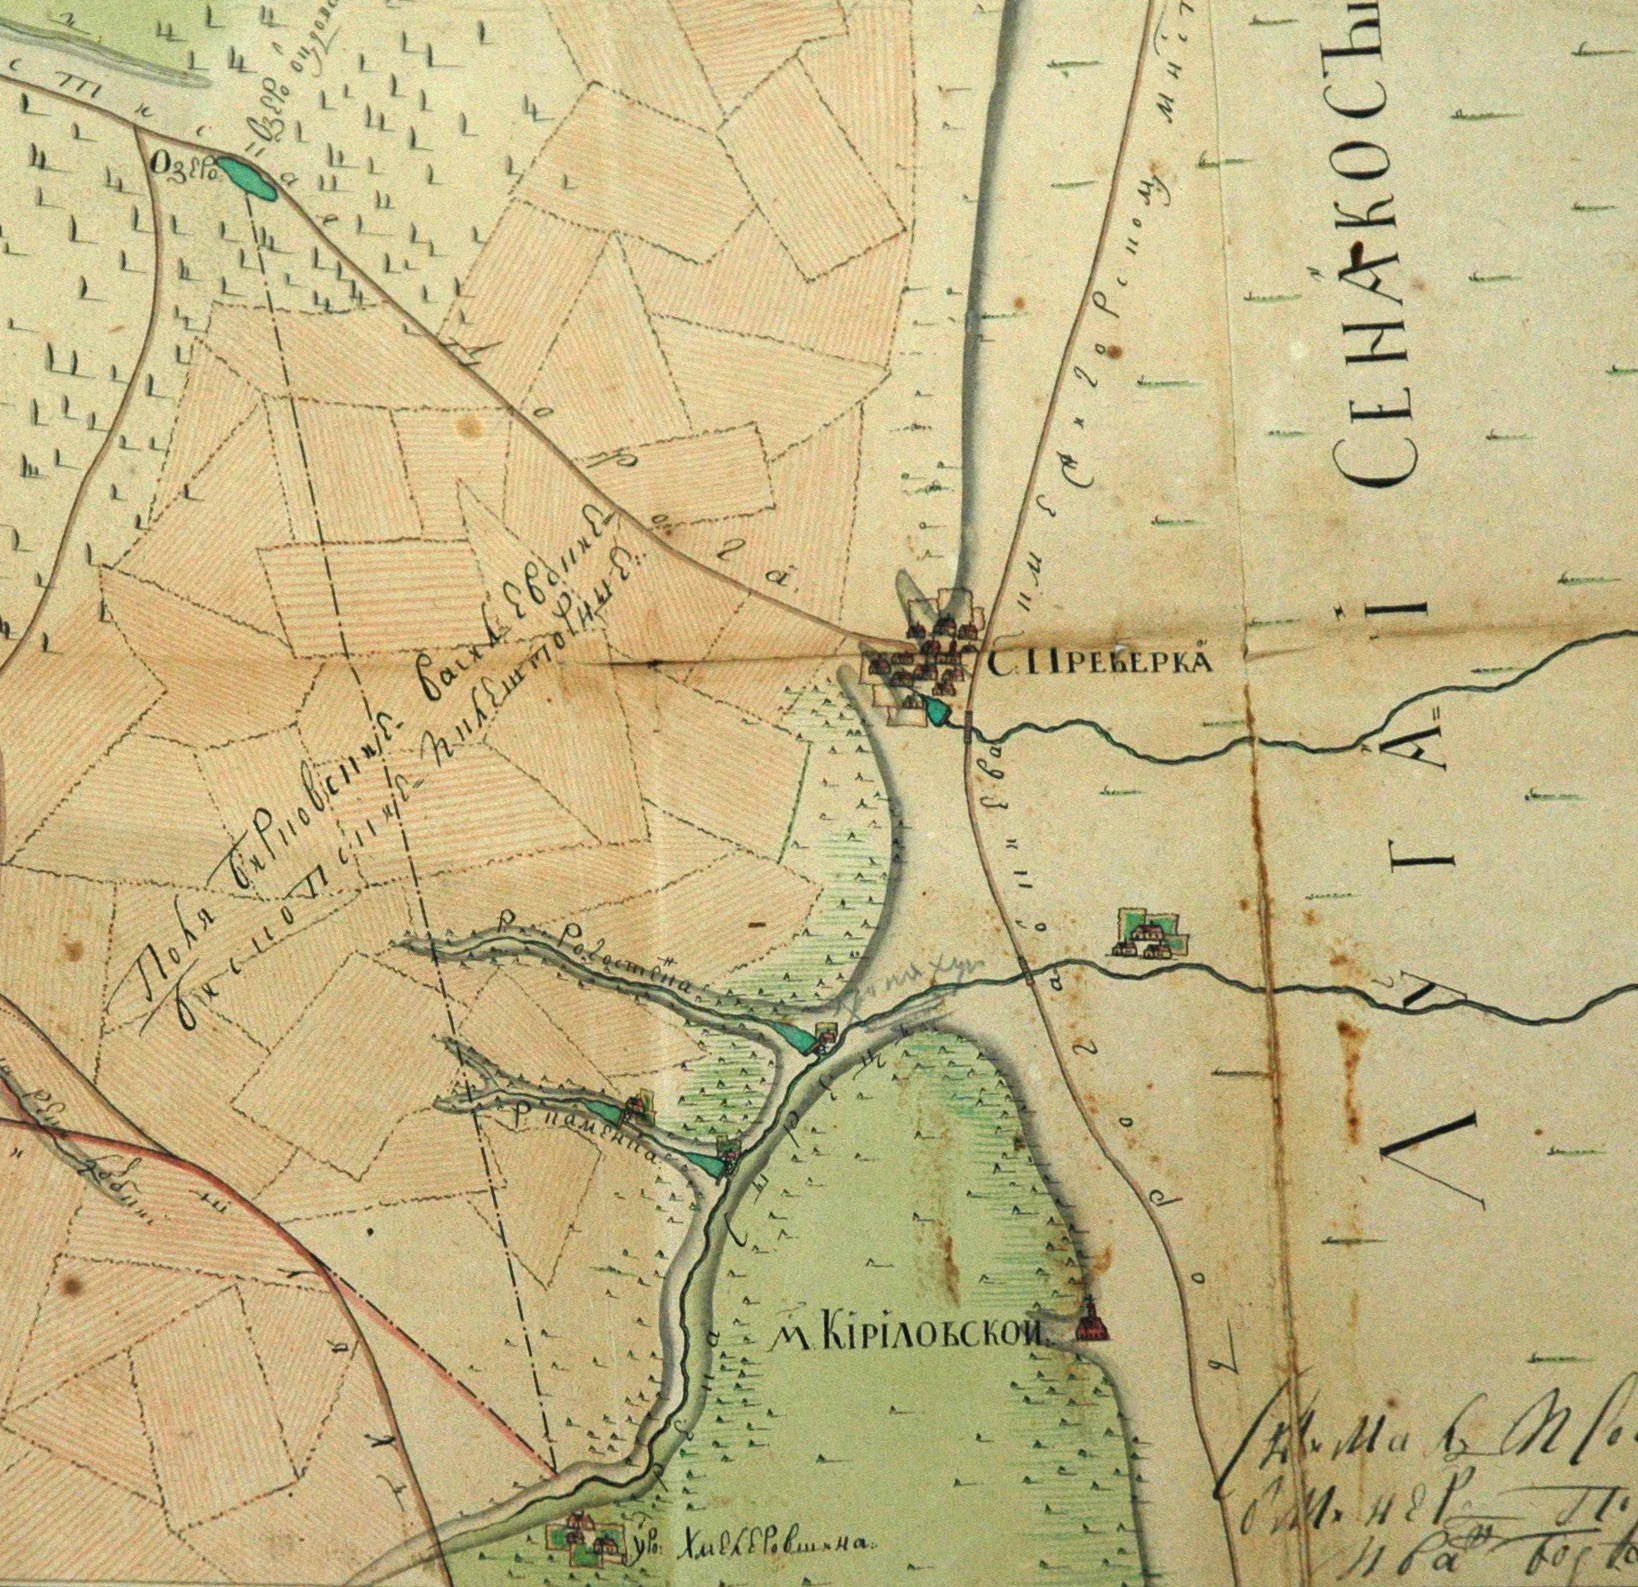
\includegraphics[width=\linewidth]{chast-colebanie-osnov/pochayna/1746-syrec.jpg}

\textit{Сырец (нижняя половина картинки) на плане 1746 года.}
\end{center}

На протяжении своего водосбора Сырец впитывает, по причине насыщенности окрестностей водой, бесчисленные ручьи и более крупные притоки – из поименованных это, справа – Каменка (исток\footnote{50°28'32.17"N 30°24'55.5"E} из коллектора начинается на окраине лесопарка Дубки, близ Саратовской улицы, проходит наискось рощи, затем струится вдоль Стеценко, ныряет под нее в коллектор и выходит в пруды на стыке Стеценко и Щусева), Рубежовский (назван так от земель одноименной колонии для малолетних, переведенной сюда в 1884 году из деревни Михайловская Рубежовка, что была в 35 километрах от Киева), слева – Рогостинка (известна по меньшей мере с 18 века, был и одноименный хутор), Курячий Брод, Западинка (эти два притока соединялись в один поток и уже затем впадали в Сырец, ныне заключены в коллектор). 

Долина Сырца то расширяется до весьма приличной долины, то сужается и ограничивается крутыми берегами. В верховьях, в парке устроены пруды. Русло то песчаное, то взято в бетон. Сливы автомобильной химии, берега, ставшие свалками.

Издавна люди на протяжении Сырца устраивали пруды и водяные мельницы при них, используя сильное течение реки. Заводились и винокурни, расходуя воду так, что на мельницы её уже не хватало. В документе 1747 года\cite[вып. 6, стр. 57]{histmatkiev} о земельных спорах между киевскими мещанами и монастырями написано:

\begin{quotation}
Жытели куренёвские и сырецкие над речкою монастырскою Сырцем по устроевали себе вынокурни и затем воде стало быть уменьшение что оную воду из речки Сырця порозбералы по вынокурнях почему мельницы монастырские напротыв прежнего сталы водою довольствоватысь.
\end{quotation}

На протяжении Сырца от улицы Ольжича по Копыловскую с 19 века работали кирпичные заводы (купчихи Христины Марр, семьи Булышкиных и других\footnote{Подробнее читайте в моей книге «Киевский кирпич».}), в крутом юго-восточном пойменном берегу добывалась глина. Поныне от этих карьеров остались глубокие озёра.

\begin{center}
\includegraphics[width=\linewidth]{chast-colebanie-osnov/pochayna/\myimgprefix les-na-syrce.jpg}
\end{center}

\newpage

\begin{center}
\includegraphics[width=0.98\linewidth]{chast-colebanie-osnov/pochayna/\myimgprefix IMG_20130812_155244.jpg}
\end{center}

\textit{2013. Ниже улицы Ольжича.}

\begin{center}
\includegraphics[width=0.98\linewidth]{chast-colebanie-osnov/pochayna/\myimgprefix IMG_20130812_164101.jpg}

\textit{2013. Пойменное озеро, бывший карьер Петровских кирпичных заводов.}
\end{center}

\newpage

\begin{center}
\includegraphics[width=\linewidth]{chast-colebanie-osnov/pochayna/\myimgprefix IMG_20130812_162049.jpg}

\textit{2013. В старинном коллекторе.}
\end{center}

\begin{center}
\includegraphics[width=\linewidth]{chast-colebanie-osnov/pochayna/\myimgprefix IMG_20130812_181739.jpg}

\textit{2013. На равнине Оболони.}
\end{center}

\newpage

Спустя пару сотен метров от змеей вьющейся под гору улицы Ольжича, Сырец прячется на несколько километров в дореволюционный коллектор, вход куда прегражден целой системой решеток, что не помешало проникнуть внутрь парочке крупных бревен.

Ежели шагать улицей Ольжича сверху, по левой её стороне есть следы некоего притока Сырца. Изучить их мне помешали местные жители. Низовье притока, глубокий овраг, превращено в мусорник. От Ольжича до входа в коллектор Сырец представляет неудержимую, почти горную реку в ущелье. Доселе могучая, тут благодаря узости берегов ускоряется еще более. Русло загажено, из берегов торчат трубы, откуда сочится всякая дрянь. 

Вдоль улицы Сырецкой, где канализационные люки пятидесятых годов и красивое, сталинских времен здание дома культуры, Сырец протекает под землей и покидает коллектор уже на Оболони, к востоку от железной дороги между улицами Вербной и Богатырской. 

Оттуда он – мелкий, широкий, успокоенный – течет к современному Кирилловскому озеру по спрямленному руслу, зажатый между промзоной и гаражами. Берега террасированы, частично укреплены бетоном. Признаков жизни в реке тут не заметно, хотя водичка с виду чистая. Только у места впадения в озеро\footnote{50°29'55.0"N 30°29'27.9"E} вьются стайки мальков.

Прямое русло Сырца от коллектора до озера Кирилловского появилось уже после начала 1960х, а прежде было было южнее\footnote{50°29'45.6"N 30°29'39.0"E}, причем следы этого старого устья сохраняются поныне, достаточно пройти пешком вдоль берега от нынешнего устья в сторону Петровки.

%На снимке 2013 года – Сырец, к востоку от улицы Богатырской, вышел из промзоны и течет по лугу к Кирилловскому озеру:

%\begin{center}
%\includegraphics[width=0.78\linewidth]{chast-colebanie-osnov/pochayna/cyrec-IMG_20130812_181735.jpg}
%\end{center}

%Сырец был и остается самым мощным западным притоком Почайны-1. 

До публикации Д. Я. Вортманом в статье «Северо-западные окрестности Киева середины XVIII в. на картах монастырских владений»\footnote{Вестник геодезии и картографии, 2015, № 4 (97), с. 38-43.} карты 1752 года, озаглавленной «Карта снятая и свидетельствованная по Дукту дьяка Алферова спорных земель по иску Киево-Кирилловского монастыря с Киевским Магистратом», можно было только вычислительным путем восстановить примерно положение некоторых урочищ около Сырца, упоминаемых в земельных документах того времени.

Скажем, в мировом соглашении между  Кирилловским монастырем и Киевским магистратом по поводу спорных земель, 1767 года, среди описания размежевания есть такое – для удобства разбиваю на пункты:

\begin{quotation}
1. В начале от самой нызшей, стоящей на речке Сирце, близ подгородья меского киевского Куренёвщины, Кирилловского монастыря мельници 

2. идучи вниз по той речки Сирцю чрез дорогу Куренёвскую, 

3. подаваясь мало в лево пройти оною же речкой сто дватцать два с половиную треаршинных саженей, 

4. а оттоль вправо на болото багнистое, називаемое Пуниское, куда быть и течение оной речки 

5. и провесть оную до того болота рвом, а от болота в сагу нижеписенную ровом же,

6. а из саги в Кривую Почайну или в озеро Ерданское тем местом, где перекопан валок, оставляя при магистрату по левой руки два сенокосы прилеглые: еден к подгородной меской Кореневской земле, а другой к сеножати Ковальской;

7. чрез тое ж багнистое болото, занимая оной по левой же руки не малую часть с сенокосцами, очеретом и лозами, поуз сенокосы Кравецкую и Кушнерскую, прозиваемые Борок, и пески к урочищу саги до вигонной земли, всему тому быть за магистратом, а в правую руку за Кириловским монастырем; 
\end{quotation}

Разберем по пунктам.

1. Началом границы положена самая нижняя по течению мельница Кирилловского монастыря, на речке Сырце, в окрестностях Куренёвки.

2. Следуя вдоль русла Сырца (не сказано, по какому берегу оного), переходим дорогу Куренёвскую. Та самая дорога, которая ныне разбита на улицы Кирилловскую (Фрунзе) и Вышгородскую. По плану Ушакова 1695 года, после пересечения дороги, на некоем расстоянии Сырец впадал в озеро Долгое Кирилловское. В документе 1767 года об озере с таким названием нет ни слова. За пересечение речки Сырца с дорогой я беру, примерно, нынешний перекресток улицы Сырецкой с Кирилловской.

3. Уже перейдя дорогу, мы продолжаем следовать тем же руслом Сырца, но отклоняясь «мало влево», и проходим 122,5 «треаршинных саженей». Казенная, или трёхаршинная сажень с 1649 года до 1835 года равнялась 217,6 см., после указанного года – 213,36. Что же, от пересечения с дорогой надо «мало влево» отмерять 122,5*217,6/100=266,6 метров.

4. И от этой точки, на некоем расстоянии справа будет «болото багнистое, називаемое Пуниское, куда быть и течение оной речки».

Поскольку по карте Ушакова мы знаем, что Сырец впадал в озеро Долгое Кирилловское, а тут «оная речка» впадает в болото багнистое Пуниское, можно сделать вывод, что Кирилловское Долгое озеро превратилось в это самое болото. Однако, как поведаю несколько далее, не всё так просто.

Урочище Пуниское (либо Пунище) часто проскальзывает в земельных документах начала 17 века как сеножать Пуниская, данная на владение земянину Войтеху Соколовскому воеводой Киевским, Константином Острожским.

5. «и провесть оную до того болота рвом» – «оную» речку или границу? Думаю, границу, ибо далее идет «а от болота в сагу нижеписенную ровом же». Граница пошла рвом в болото, а из болота – в сагу (протоку, канал). Сага же описывается ниже, в пункте 6.

6. «а из саги в Кривую Почайну или в озеро Ерданское тем местом» – вот это очень важно! Сага из болота Пуниского – и Кривая Почайна. Хотя я не рассматриваю описание границ как непрерывный водный путь, однако здесь ясно усматривается соседство саги и Кривой Почайны. А ведь отсюда на север до Улуково весьма далеко.

Озеро Ерданское же – следующий к югу от саги, впадающий в Почайну-1 крупный водоем. «Где перекопан валок» – валок известный по множеству земельных документов Соколовского, где границы надела с одной стороны определены «валком», а с другой «потоком от церкви святого Миколы Иорданского» – к последнему мы еще вернемся в следующих главах. В бумагах, относящихся к Соколовскому, постоянно говорится еще про озеро Коссор либо Косор, «за песочем над Днепром лежачее», и соседствующее с Пуниской сеножатью и Косором урочище Борок.

На карте 1752 года картина несколько проясняется – к тому же карта снабжена подробным описанием в левом нижнем углу.

\begin{center}
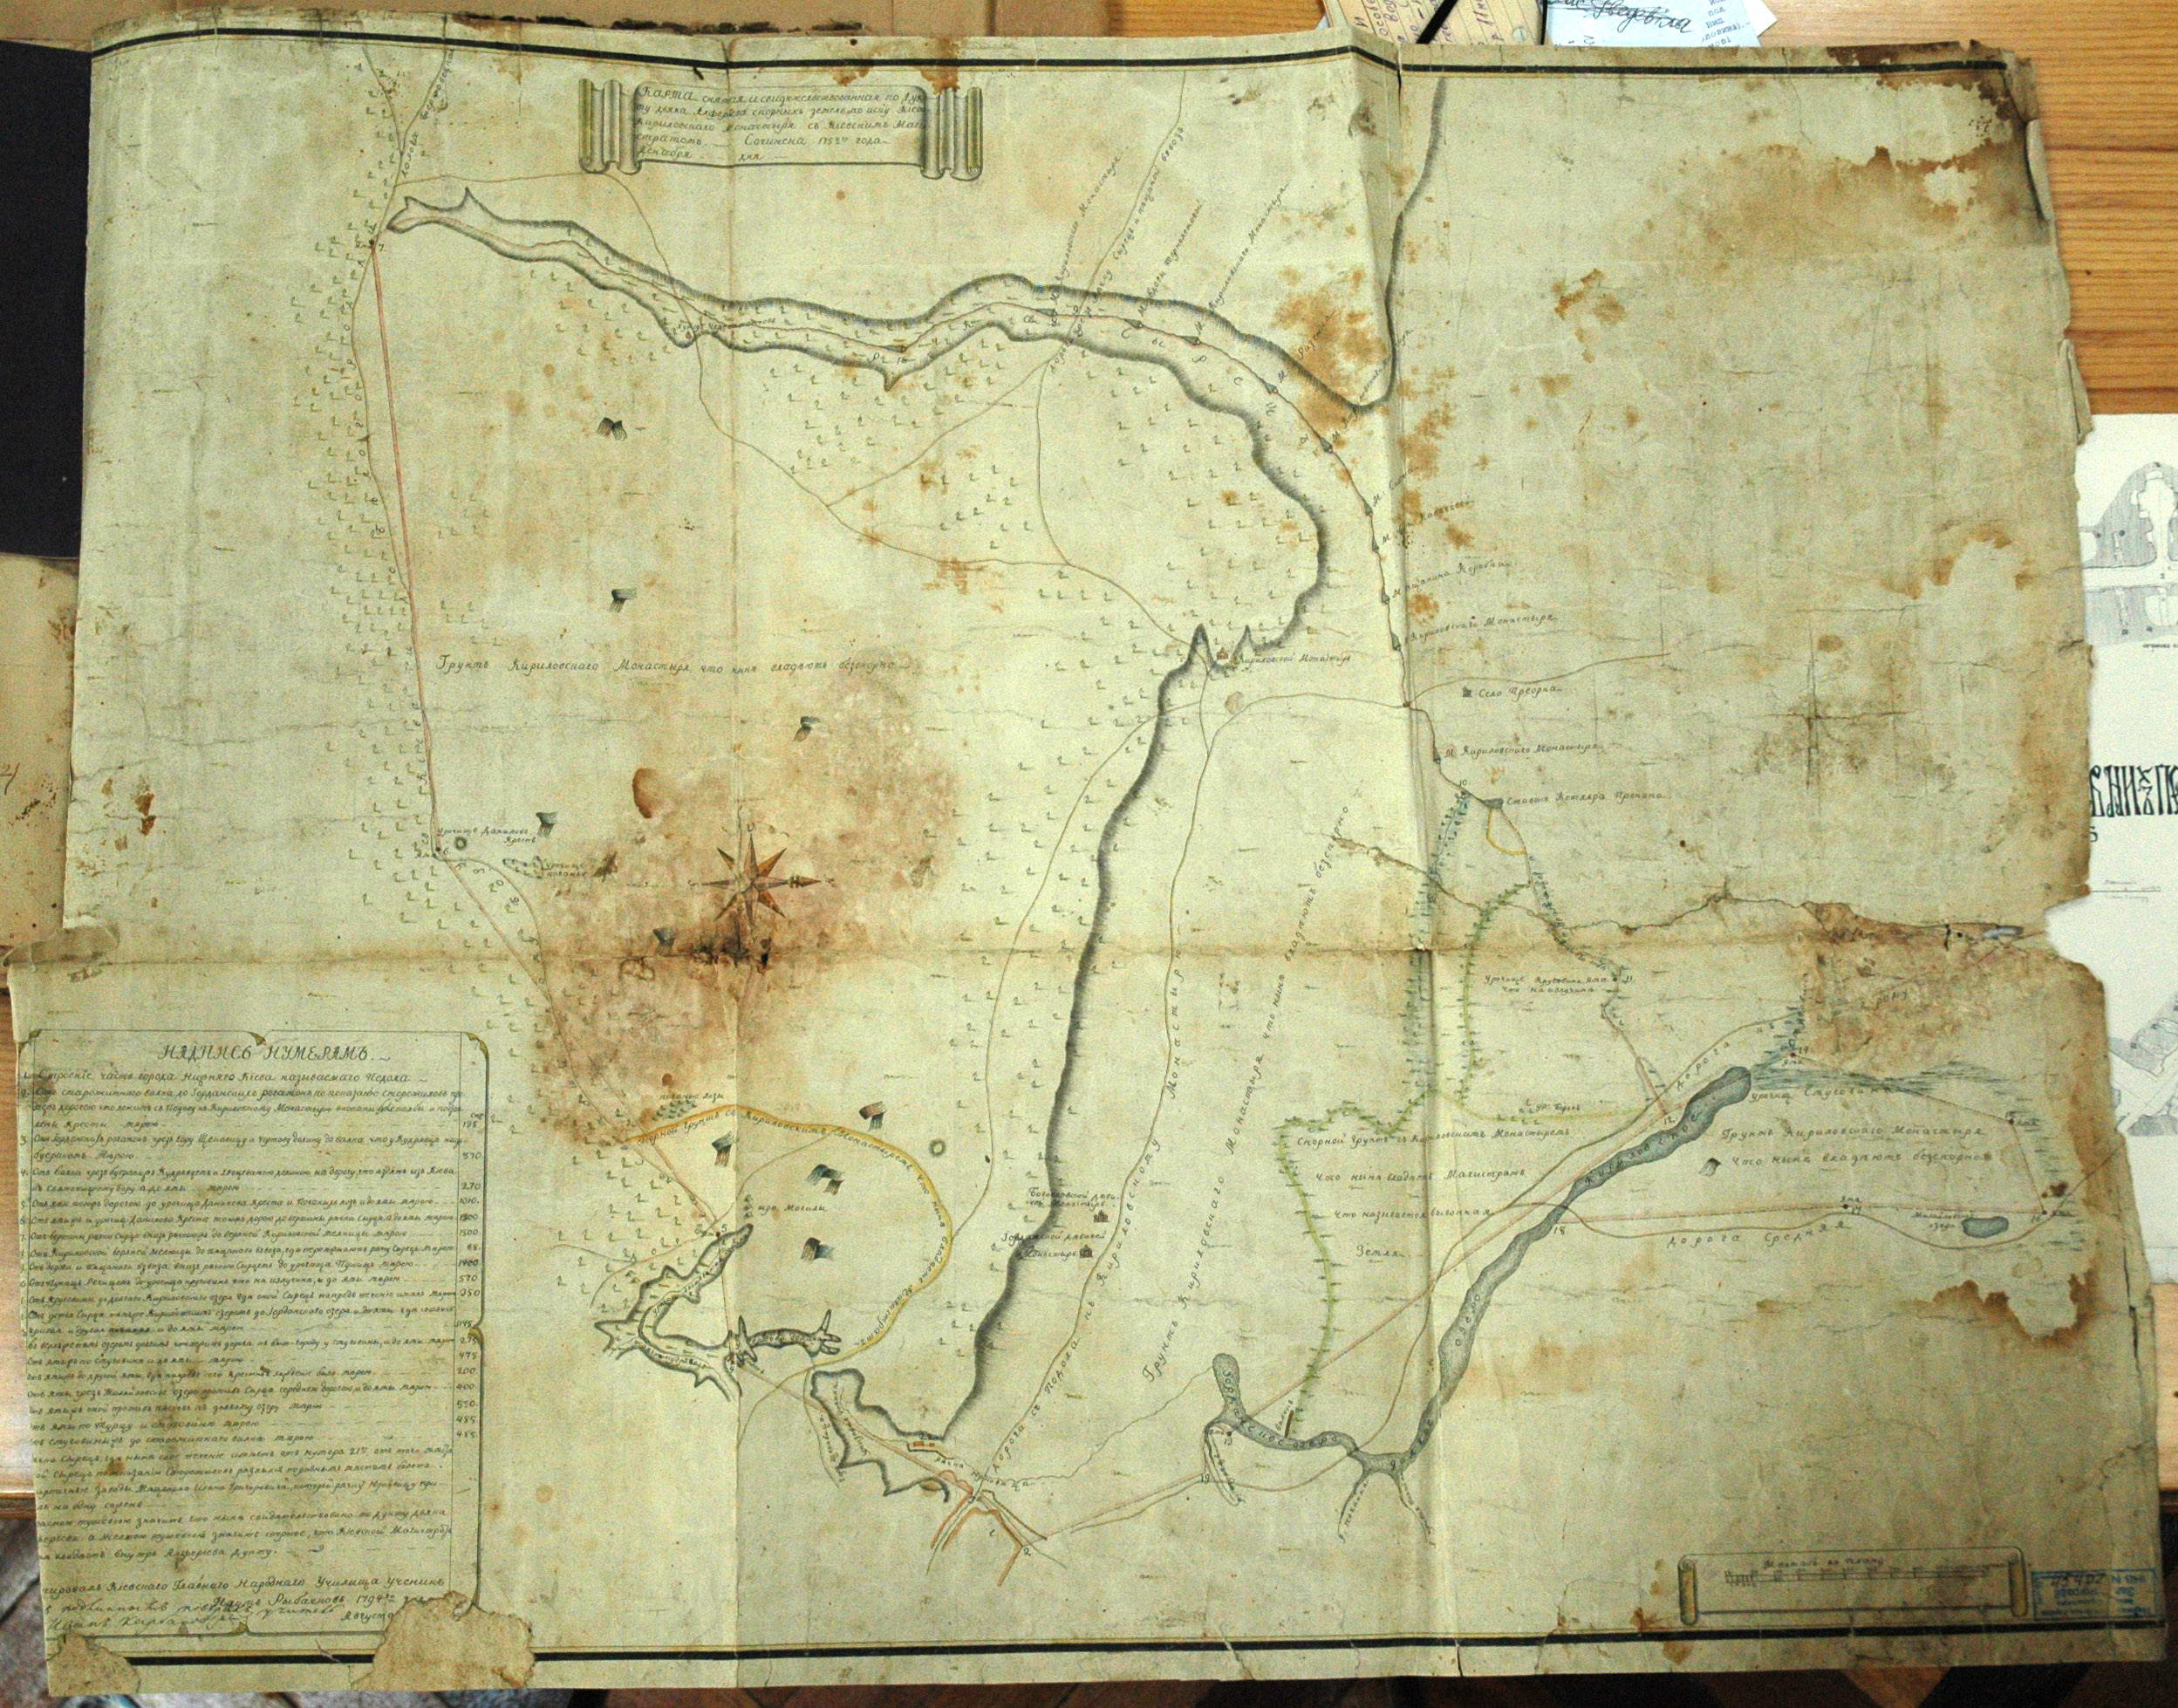
\includegraphics[width=\linewidth]{chast-colebanie-osnov/pochayna/map1752.jpg}
\end{center}

Сначала дам общий обзор карты. Ориентация ее такова, что север находится справа. Показано всё русло Сырца, Кирилловские высоты, Приорка, часть Почайны-1.

Почайна-1 как река обозначена только в низовьях, ближе к Подолу. Остальные отрезки того, что мы в 21 веке считаем Почайной, обозначены совершенно иначе, хотя еще на плане Ушакова это была цельная река.

Почти до диагонали карту 1752 года пересекает Сырец с бесчисленными прудами с мельницами на нем. 

Русло Почайны в нижнем правом углу карты представлено составным водоемом. Выше по течению от впадения в него Сырца, есть развилка русла, и подпись «урочище Смуговина», а также слово «смуговина» вдоль уходящего оттуда русла наверх. Ниже Смуговины, начинается озеро Кириловское Долгое...

Вот здесь неожиданность! Озером Кириловским Долгим явно подписана часть русла, на плане Ушакова слывущего Почайной. Итак, озеро Кирилловское Долгое с плана Ушакова (предшествующее Почайне) просто исчезло, вместо него Сырец почти напрямую впадает в основное русло Почайны, именуемое тут озером Долгим Кириловским.

Но разберем кусок карты подробнее.

\begin{center}
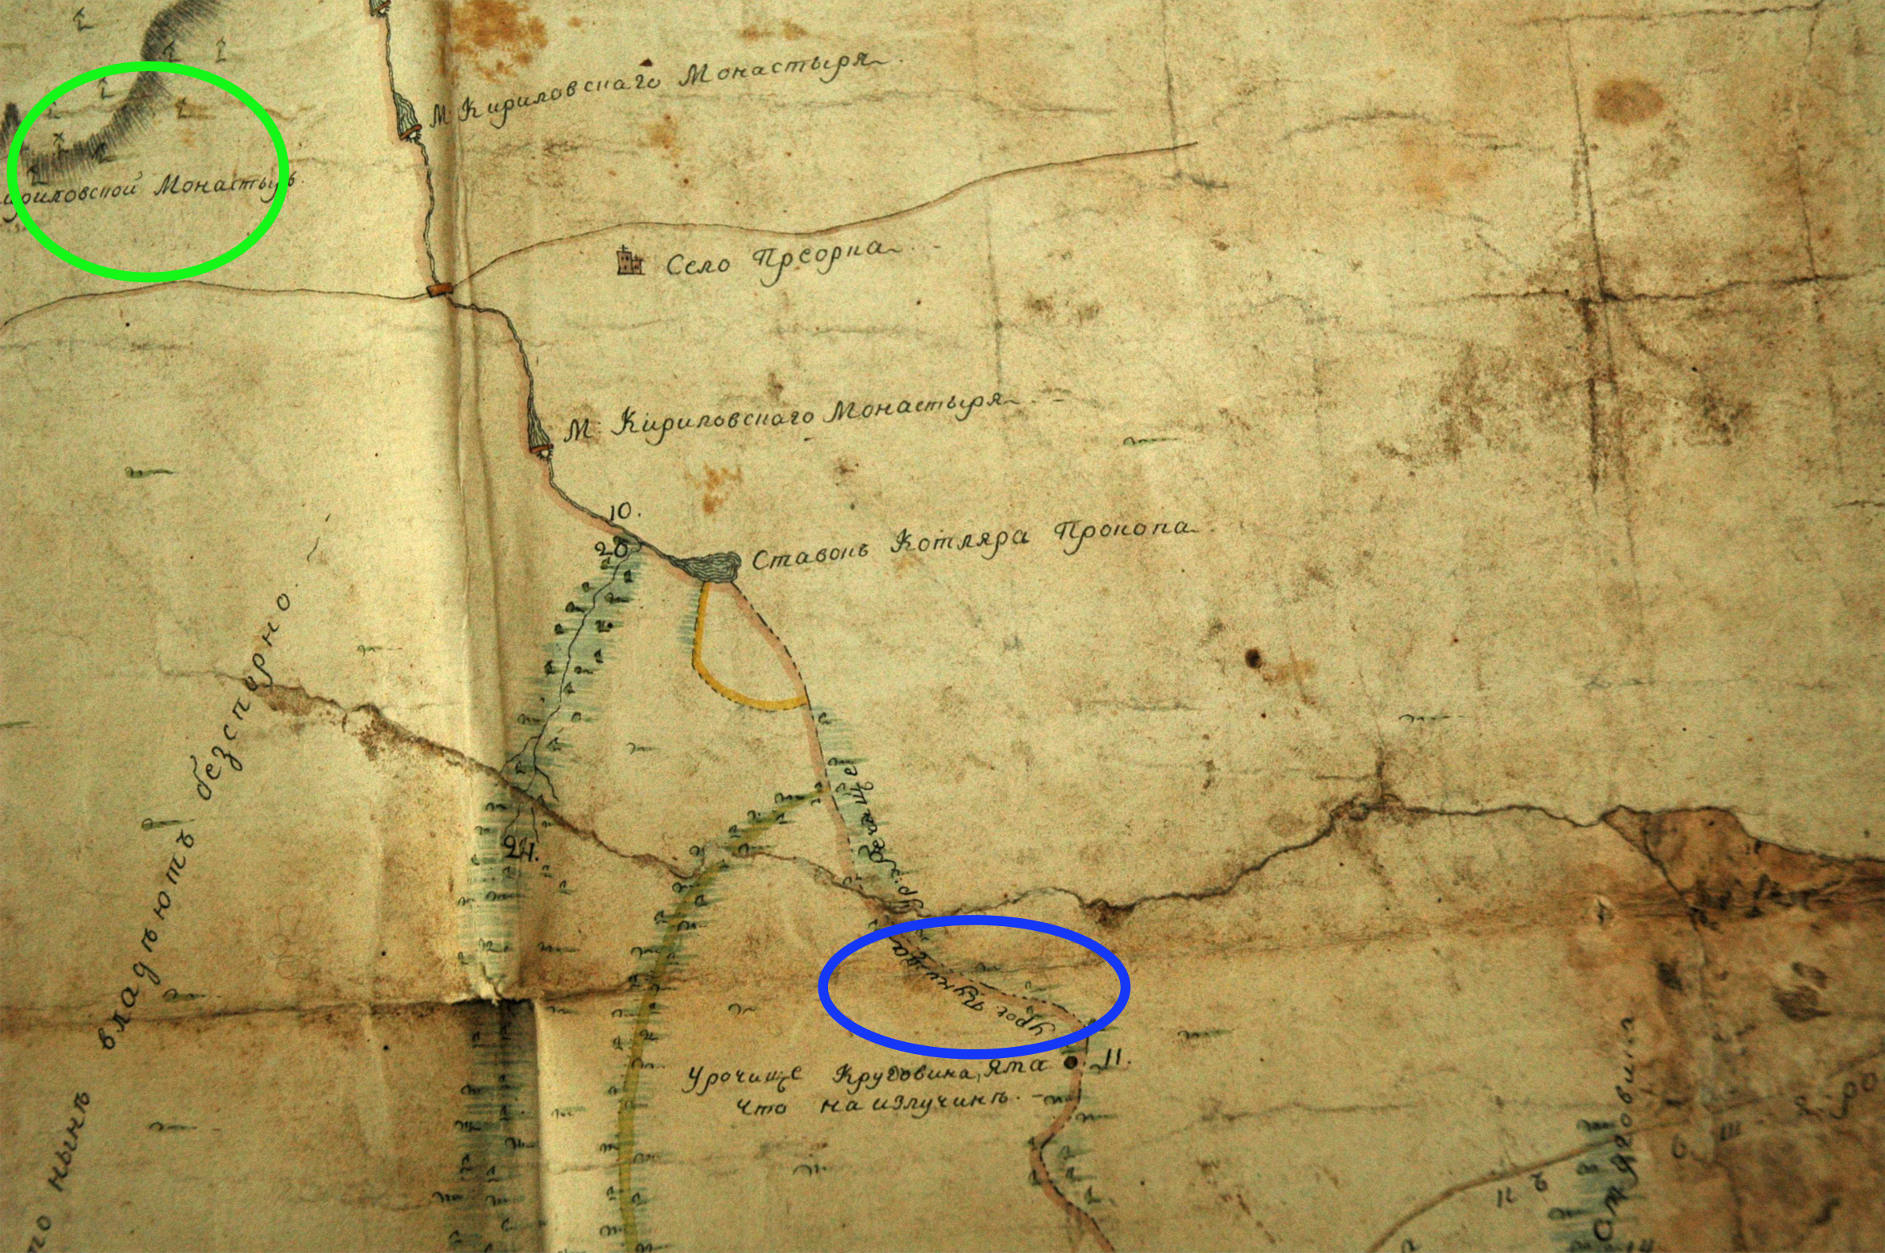
\includegraphics[width=\linewidth]{chast-colebanie-osnov/pochayna/1752-pun.jpg}
\end{center}

Салатовым я обозначил Кирилловский монастырь, синим – «урочище Пунища». Ниже села Преорки видно одну из мельниц Кирилловского монастыря, затем – став Прокопа Котляра, далее идет урочище Речище, затем Пунища, и «урочище Круговина, что на излучине». Ниже его по течению Сырца – уже устье, в озере Долгом Кириловском (на картинку не влезло). Можете рассмотреть этот же кусок на общей карте, ниже Преорки.

Как это понимать? Пропажа Долгого Кирилловского озера как водоема, обозначенного на плане Ушакова, сыграла на руку Кирилловскому монастырю, ибо по описанию урочищ, Сырец впадает в озеро Долгое Кирилловское. При исчезновении прежнего водоема с таким именем, имя перешло на следующий по течению водоем, кстати больший, нежели прежнее озеро Долгое Кирилловское.

Сие толкование возможно, если план Ушакова верен в изображении устья Сырца. 

По грамоте 1694 года (за год до составления карты Ушакова) нам известны «озера прозываемые: Три тони, Долгое и Узкое, и озеро Василевское», причем с Тремя Тонями можно соотнести Улуково, а Долгое и Узкое (это одно озеро, не два) «взялось от Киева и кончится в озеро Три-тони». Значит, с Долгим и Узким сопоставляются Долгое Кирилловское с карты 1752 года, и некое русло выше его по течению, вероятно обозначенное как «Смуговина», направленная вверх.

В грамоте 1694 года есть озеро «Долгое и Узкое», однако не «озеро Долгое Кирилловское». Это два разных названия, закрепленных за двумя разными водоемами.
 
Попытаемся подобрать ключик к загадке и всё распутать. В документе 1717 года\cite[вып. 6, стр. 59]{histmatkiev}, о впадении Сырца в Кирилловское озеро сказано:

\begin{quotation}
Речка Сырец давным своим течением в долгое озеро Кыриловское было упадает, а ныне как Прокоп Котляр, жытель Куреневский, роскопал оную речку Сырец, и ставок и сеножатку себе на грунте монастырском зделал, то оная речка Сырец не по старому течение свое возимела, ибо оной Котляр воду речки Сырца справыл на грунта монастырские, и потому грунт монастырский, какий был по сей стороне речки Сырця от монастыря, стал быть за речкой Сырцем, почему мещане оной грунт монастырский себе прысволяют неправедно, и речка Сырец в долгое озеро уже невпадает, но по грунтам монастырским розолялся.
\end{quotation}

Что же? Давним своим течением Сырец впадал в Долгое озеро Кыриловское. А Прокоп Котляр – вспомним про его став на карте 1752 года – изменил русло Сырца, «и речка Сырец в долгое озеро уже невпадает, но по грунтам монастырским розолялся».

Думаю, причину исчезновения Долгого Кирилловского озера – водоема, изображенного на плане Ушакова – мы нашли. Прокоп Котляр лишил этот водоем питания. И Сырец по равнине пошел как-то иначе, огибая прежнее озеро, причем заболотилась местность у Пунища. На плане 1752 года видно, как русло Сырца проходит после става Котляра урочищами Речище, Пунище, Круговиной до того русла, что на плане Ушакова обозначено Почайной, а на плане 1752 года – озером Долгим Кирилловским. А в грамоте, составленной за год до плана Ушакова, судя по всему этот же отрезок Почайны именуется как «озеро Долгое и Узкое». 

Нетрудно было, при том, что озеро Долгое Кирилловское осталось где-то в стороне от течения Сырца, перенести название «Долгое Кирилловское» на водоем, слывущий как «Долгое и Узкое», с выгодой для Кирилловского монастыря и полагаю каких-нибудь чиновников.

Современные Иорданское и Кирилловское озера – это раздувшееся русло Кирилловского Долгого озера с плана 1755 года.

\textbf{Кирилловский ручей}. Следующий по счету от Сырца, к югу, западный приток Почайны-1. Течет из Бабьего яра в коллектор.

\textbf{Ручей из Репяхового яра}. Репяхов Яр – почти такой же глубокий яр, как Бабий. Вот так Бабий Яр, к югу холм с Кирилловской церковью, и еще к югу – Репяхов яр. О нем мы подробно поговорим дальше, в части про Логово Змиево. По Репяховому яру тоже бежит ручей, и до создания Подольского спуска он еще был на поверхности, через него существовал мост около стадиона Спартак. Ныне ручей заключен в коллектор.

Кирилловский ручей и ручей из Репяхового яра, сойдя на равнину Оболони, сворачивали на юго-восток и, вскоре соединившись, единым потоком несли воды свои к давнему, долгому, направленному от Кирилловских высот на северо-восток, озеру Иорданскому (Чернечьему). А оно вливалось в Почайну-1. Современный выход воды обоих ручьев из коллектора – залив Волковатый.
 
\textbf{Ручей Иорданский и оспаривающие имя Юрковицы}. Об этих западных притоках Почайны-1 расскажу подробно в главах про Кирилловские высоты. Все сейчас в коллекторах, один к северу от Иорданской церкви, на земле садового товарищества «Кожевник», другой вытекает из Мыльного переулка, третий в яру между Щекавицей и Юрковицей, по улице Нижнеюрковской. Ручьи впадали в озеро Иорданское.

\textbf{Иорданское озеро, оно же Чернечье}, лежало на лугах в некотором отдалении напротив Иорданского монастыря, а позже одноименной церкви, между оной и руслом Почайны-1. К восьмидесятым годам 19 века на его берегах появилась скотобойня и скотомогильник. Тогда же, озеро уже не соединялось с низовьем Почайны естественно. Вместо этого от озера прорыли канал к заливу, прообразу Гавани в вершине Подола. Туда же тянулась и «ниточка» от окончания русла Почайны-1.

В 20 веке старое Иорданское-Чернечье озеро стало исчезать – его вытеснила железнодорожная станция Киев-Петровка с одной стороны, а с другой увеличиваемая на запад Гавань. К сороковым годам от него остались рожки да ножки – несколько водоемов в окрестностях выхода из станции метро Петровка, что ближе к книжному рынку на улице Вербной, особенно на юг оттуда по месту современного западного конца Гавани. Современное Иорданское озеро – в другом месте, в непомерно раздувшейся прежней части Почайны-1.

На плане 1752 года хорошо показано Иорданское и его окрестности.

\begin{center}
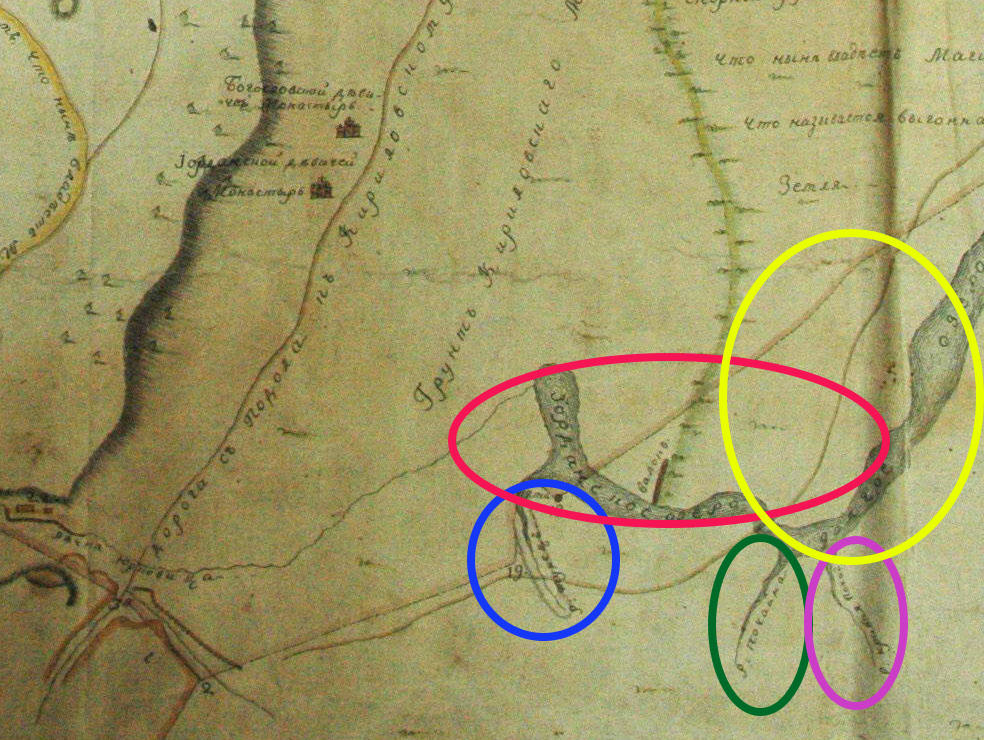
\includegraphics[width=\linewidth]{chast-colebanie-osnov/pochayna/1752-chern.jpg}
\end{center}

Цветными окружностями я отметил следующее.

Желтый – озеро Долгое Кирилловское. 

Красный – Иорданское. 

Зеленый – «р. Почайна». 

Синий – «р. Турец». 

Малиновый – «р. Кривая Почайна».

Кривая Почайна по некоторым из рассмотренных нами документов протянулась от Улуково до Васильевского озера, а по другим – находится ближе к Подолу. Значит, либо существовало два одноименных водоема, либо обе Кривые Почайны – части одного распавшегося большого водоема\footnote{Кроме Почайны Кривой, была также некая Почайна Пещаная. Если это не участок Кривой Почайны по месту «озера Пичани» с плана Шуберта, то возможно – название Ицуна. Почему? Когда от верховья Ицуна переправлялись на другой берег Днепра, на остров Осещину, то приставали в урочище Соплик. Там же была и речка Соплик. А Почайна Песчаная упоминается как соседствующая с Сопликом, но по другую сторону Днепра. А там начинался Ицун.

Из протокола действий межевой Комиссии, назначенной для решения спора о границах между Межигорским монастырем и киевскими мещанами, 10 октября 1713 года:

\begin{quotation}
от тое зась Соплика в Днепр поперек, аж знову до Почайны речки пещаной, то тут вже с Киевом граница.
\end{quotation}

В любом случае Почайна Пещаная, согласно документу, была где-то в верховьях, на уровне устья Десны, раз упомянут остров Осещина.}. Увы, по карте 1755 года нельзя сказать, куда и что впадает ниже.

\textbf{Турец}. Соединялся с Иорданским озером ниже ручья Юрковицы. 

Под нынешней улицей Туровской (в современных пределах известной по крайней мере с 19 века) ныне в трубе протекает ручей, который диггеры считают Турцом. Он впадает в коллектор Юрковицы. На картах 19 века вдоль Туровской улицы никакой ручей не показан. 

Судя по плану 1901 года, опубликованном в сборнике «Труды русских водопроводных съездов: съезд пятый. 18-25 марта 1901 года в Киеве», Турец был поглощен Гаванью: 

\begin{center}
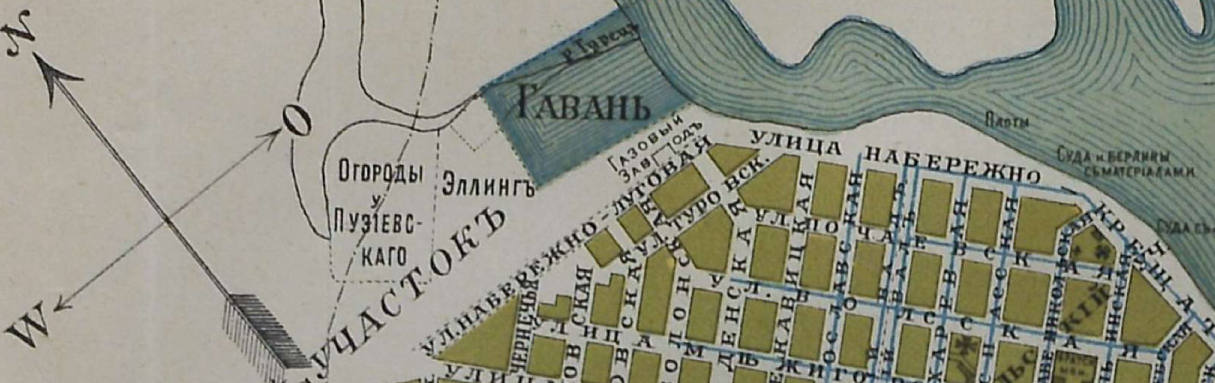
\includegraphics[width=\linewidth]{chast-colebanie-osnov/pochayna/1901-turec.jpg}
\end{center}

На плане, левее от Гавани, над «огородами Пузиевского» – Иорданское озеро. В документе 1767 года сказано: «а озером Ерданским пришед к смуговине Турцу, не идучи тем Турцем, но прямо с начала оного Турца к полисаду на рог полисада, где земля выгонная окончивается». Полисад это бревенчатая стена, ограждавшая Подол.

%Николай Шарлемань в статье 1967 года «Речка Почайна теперь и прежде» отмечал, что «в 1912 году закрыт был проток Торец, заливавший «Ковш», где было частное пароходостроение, и углубили гавань, существовавшую с 1898 года».

%Рог, угол полисада виден на плане левее зеленого кружочка. 

Вот мы и подобрались наконец к Подолу. Рассмотрим притоки, которые должны были вливаться в Почайну-2.

\textbf{Глубочица или Кудрявец}. Ближайший к югу от Гавани приток Почай\-ны-2.

Раньше, как можно судить по старинным земельным документам, эта речка слыла Кудрявцем, и овраг с нею назывался так же. Глубочицким же яром именовался какой-то другой овраг в окрестностях, либо просто урочище, ближе к улице Соляной и даже Нижнеюрковской. И оттуда имя Глубочицы переползло на Кудрявский яр, а заодно и на речку. Далее я пользуюсь современными привязками названий к водоемам.

Однако полезно обратиться к той же замечательной карте 1752 года.

\begin{center}
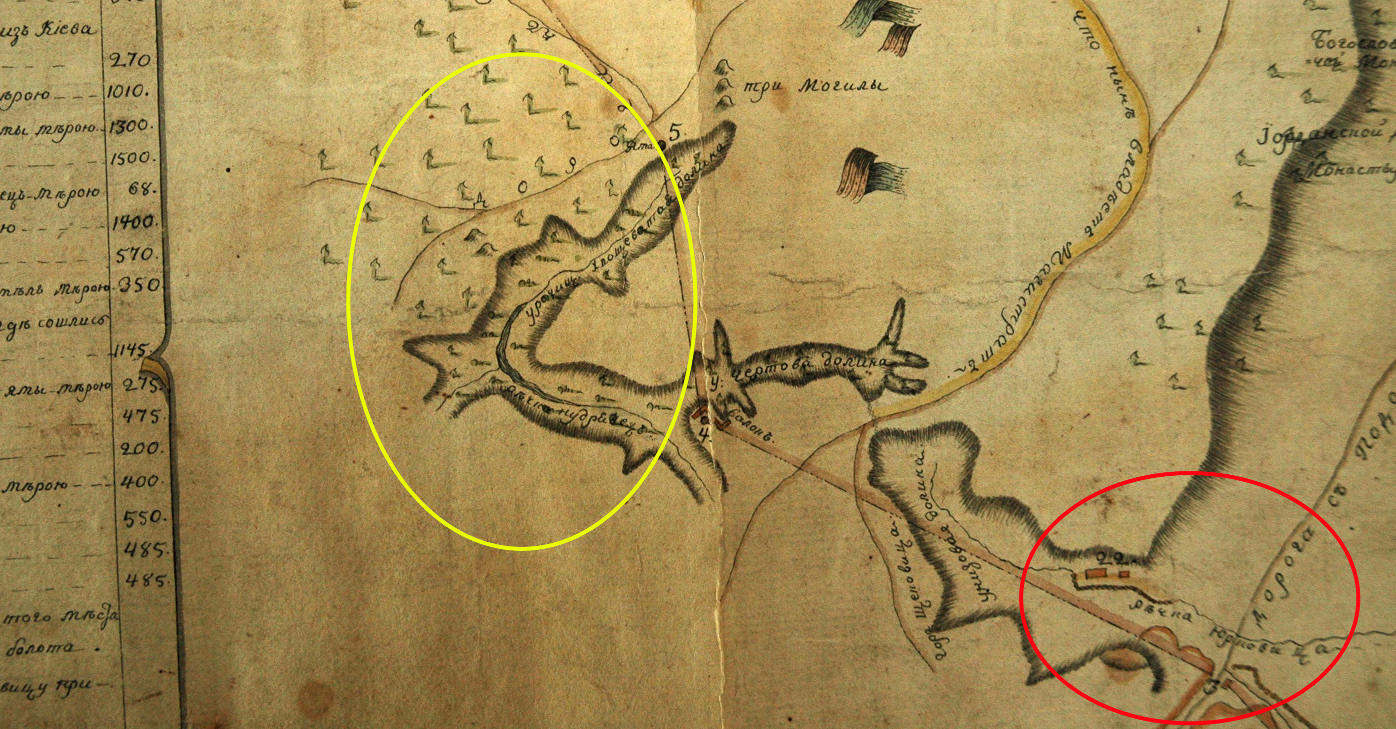
\includegraphics[width=\linewidth]{chast-colebanie-osnov/pochayna/kudr.jpg}
\end{center}

Мы еще выжмем из нее и другие важнейшие сведения, пока же двумя овалами я отметил следующее.

Красный – ручей Юрковица, там сейчас улица Нижнеюрковская.

Желтый – там две подписи: «урочище Хвощеватая долина» и «речка Кудрявец». Местность в желтом овале точно вписывается в современные очертания русла взятого в коллектор ручья, известного как Глубочица, в пределах начиная от истока на «даче Хрущова», и эдак до улицы Соляной. Очень узнаваемый полукруг.

Открытый исток Глубочицы можно увидеть в мрачном овраге на Даче Хрущова – парке в усадьбе Института педиатрии, акушерства и гинекологии, через дорогу напротив парка Котляревского. Мы сняли это в фильме «Киевская сюита». Вообще у Глубочицы два истока, в отрогах Кмитова яра – первый вытекает из трубы в цепь прудов на Даче Хрущова, второй из околиц Цветущего переулка и по улице Кмитов яр (один из отрогов одноименного яра), и затем они соединяются. Кмитов яр называется по имени владельцев, дворян с фамилией Кмит, которые в 1829 году купили там землю. Пройдя в низовье яра под заводом Артема и улицей Татарской, речка в коллекторе выруливает к улице Глубочицкой, проложенной по дну одноименного оврага, где она и протекала до Подола вдоль горы Щекавицы.

%Возможно, у нее был около Лукьяновки левый приток – не знаю, впадает ли он в коллектор Глыбочицы. 

По 2014 год, некий звонкий ручей в своем коллекторе стекал вдоль длинной лестницы с горы по частному сектору (усадьбы 25, 27, между улицами Печенежской и Соляной, в сторону гаражного кооператива «Соляной»). Насколько я понимаю, именно яр, где проходит Соляная улицы, обозначен на карте 1752 года как Чертова долина. По Соляной тоже протекал большой приток Глубочицы, и вероятно упомянутый ручей либо его начало, либо вливается в приток.

Немного выше от Соляной по течению, был пруд, в удолье между улицами Татарской и Глубочицкой, к югу от стоящих на пригорке домов 2-А, 2-Б, 2-В по Татарской. В этой котловине, где с конца 2015 по осень 2016 шустро возвели жилой комплекс, в советское время был дрожжевой завод, а до революции – водочный завод Чоколовой. Винокурни-то на реках строили!
\vspace*{\fill}
\begin{center}
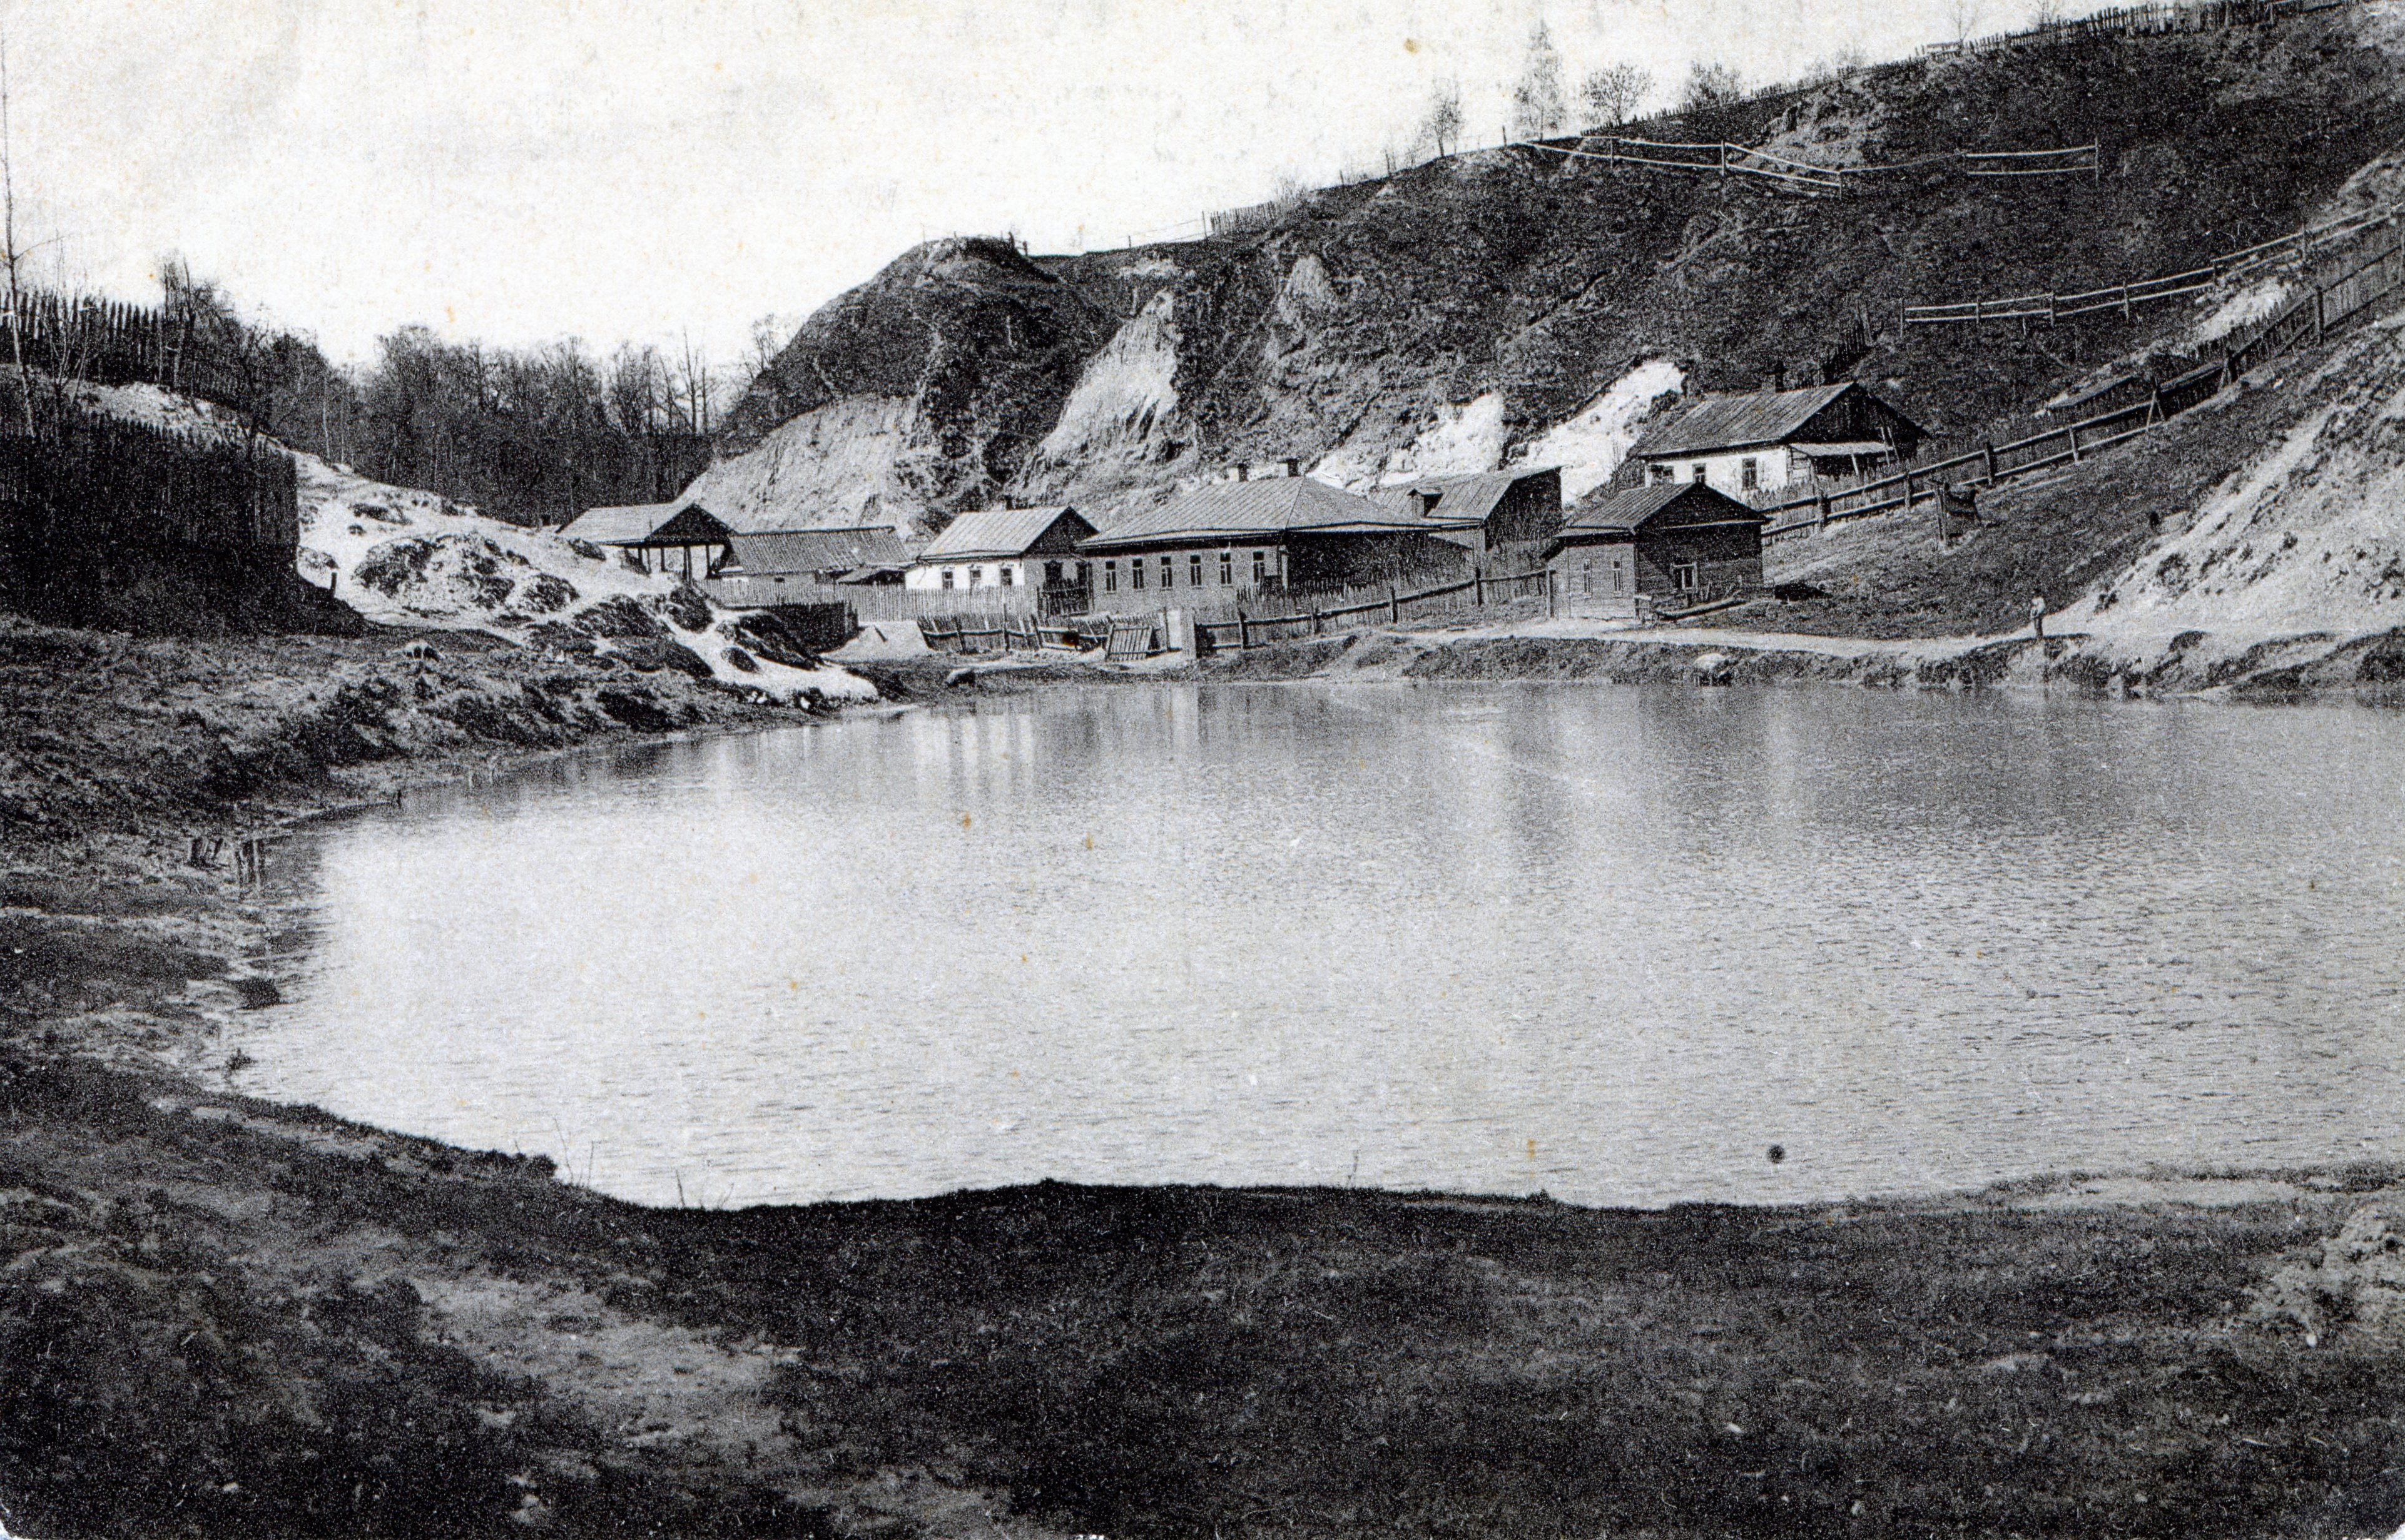
\includegraphics[width=\linewidth]{chast-colebanie-osnov/pochayna/tatarsk-stavok.jpg}

\textit{Пруд при заводе Чоколовой.}
\end{center}
\vspace*{\fill}
\newpage

Долго, долго эта котловина на территории дрожжевого завода пустовала, огражденная забором. Снимки лета 2013 года, снятые с Татарской улицы. Вид с запада: 

\begin{center}
\includegraphics[width=0.95\linewidth]{chast-colebanie-osnov/pochayna/\myimgprefix IMG_2628.JPG}
\end{center}

\begin{center}
\includegraphics[width=0.95\linewidth]{chast-colebanie-osnov/pochayna/\myimgprefix IMG_2630.JPG}
\end{center}

\newpage

Застройка котловины в декабре 2015 года, вид с севера, от дома по Татарской, 25-Б:

\begin{center}
\includegraphics[width=\linewidth]{chast-colebanie-osnov/pochayna/\myimgprefix IMG_20151212_140355.jpg}
\end{center}

\begin{center}
\includegraphics[width=\linewidth]{chast-colebanie-osnov/pochayna/\myimgprefix IMG_20151212_140318.jpg}
\end{center}

\newpage

Правый приток Глубочицы-Кудрявца, ручей с современным названием Кудрявец, под землей впадает в Глубочицу от Кудрявского спуска. В 18 веке чуть ниже устья сего ручья, Кудрявец исконный перегораживала плотина с большим прудом и мельницей.

%Еще один правый приток Глубочицы – Киянка – длиной около 700 метров, вытекает из урочища Кожемяки и, когда русло было естественным, впадала в Глубочицу несколько южнее перекрестка улиц Смирнова-Ласточкина (ныне Вознесенский спуск, застраивается новыми домами, а был глухой улицей с полуразрушенными усадьбами и древней пещерой в суглинном склоне) и Глубочицкой, на уровне дома 7/9 по Нижнему Валу и 4-А, 4-Б по Верхнему Валу. Оттуда усиленная Глубочица шла ровно, под названием Канавы, в спрямленном русле к самому Днепру, между улицами Верхний и Нижний вал.

Еще один правый приток Глубочицы – Киянка – длиной около 700 метров, вытекает из урочища Кожемяки и, когда русло было естественным, впадала в Глубочицу несколько южнее перекрестка Вознесенского спуска и Глубочицкой, на уровне дома 7/9 по Нижнему Валу и 4-А, 4-Б по Верхнему Валу. Оттуда усиленная Глубочица шла ровно, под названием Канавы, в спрямленном русле к самому Днепру, между улицами Верхний и Нижний вал.

Киянка протекала вдоль современной Кожемяцкой улицы, в противоположной стороне от холма Киселёвки. Исток Киянки – у восточного склона горы Воловни (по ней проложен Вознесенский спуск), то бишь под холмом с Академией Изобразительного Искусства. Киянка жива и течет в коллекторе. В 2015 году ее часть при очередном строительстве пробилась на поверхность в самой середине Воздвиженки, образовав даже болотце с камышом.

\begin{center}
\includegraphics[width=0.85\linewidth]{chast-colebanie-osnov/pochayna/\myimgprefix IMG_20151004_144051.jpg}

\textit{Октябрь 2015, болотце.}
\end{center}

Старинные письменные источники о Киянке молчат. Дошедшие до нас сведения о ней впервые возникают в книгах краеведов 19 столетия. Вернемся же ко Глубочице.

\begin{center}
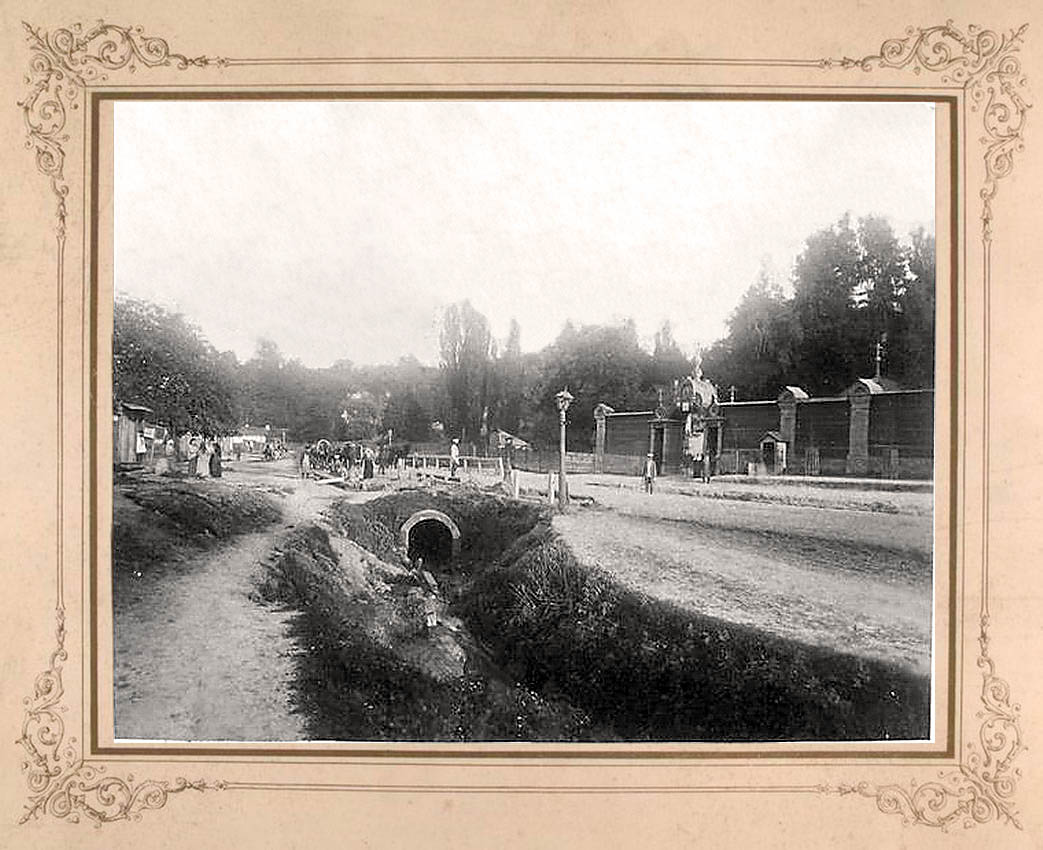
\includegraphics[width=\linewidth]{chast-colebanie-osnov/pochayna/glub-01.jpg}

\textit{В дореволюционном альбоме про женский Покровский монастырь помещен снимок монастырской стены, обращенной ко Глубочице.}
\end{center}

Известно очень мало ее фотографий. Обычно это виды с окрестных гор на Житний рынок или Крестовоздвиженскую церковь, и там при желании можно разглядеть – а скорее, угадать – ручей за мрачными деревянными постройками.
 
Ниже слияния Киянки и Глубочицы, но выше Житнего рынка, находился обсаженный вербами пруд с мельницей. Это было прежде возни со спрямлением и коллекторами, когда Глубочица протекала по Подолу иначе – тоже вдоль Щекавицы, но затем несколько огибала севернее, в сторону улицы Ярославской. 

До знаменитого подольского пожара 1811 года русло Глубочицы от места слияния с Киянкой и пруда неоднократно подравнивали, а уже после 1811-го пруд исчез, а поток воды заточили в выпрямленное русло-канал с валами по обе стороны – потому и название улиц Верхний и Нижний Вал. Сперва было красиво, вдоль речки шел бульвар.

Затем Глубочицу на этом протяжении загадили и стали называть Канавой. Вдоль Канавы стояли публичные дома, как и по Андреевскому спуску. Канава разрезала площадь Житнего торга пополам, через речку был перекинут мост. Она служила источником болезней. Газета «Киевлянин» в 1867-х писала:

\begin{quotation}
от горы и до Днепра проходит канава и, служит стоком нечистот, а под мостиками – общественным ватерклозетом, распространяет на всем своем течении едва ли способствующие общественному здоровью газы.
\end{quotation}

В начале 1870-х Канаву в пределах Нижнего и Верхнего Валов спустили в подземный коллектор. Глубочица впадает ныне Днепр в районе Гавани\footnote{В 2021-м – чуть к северо-западу от заброшенного Вантового моста у конца Нижнего и Верхнего валов).}.

Не касаясь давнего прошлого этого водоема и чехарды с Почайной-2, скажу, что Гавань, как можно судить по приведенному ранее сравнению карт 1786 и 1843 годов, состояла из старицы Днепра, по месту прежнего его русла вдоль северо-восточного побережья Подола. Эту старицу называли Оболонским заливом. В 1897-1899 годах правительство вбухало кучу денег для углубления русла и устроения там Гавани имени Николая II. На карте 1937 года Гавань еще не поглотила остатки старого Иорданского озера, но затем расширилась и на него.

Какие существовали западные притоки Почайны-2 южнее Глыбочицы? Это, во-первых, ручьи, о которых я рассказал в главе про Боричев Ток.

А самым южным притоком был источник Хрещатик (Крещатик), возле нижнего памятника князю Владимиру, известного также как колонна Магдебургскому праву. На карте Ушакова, Почайна-2 и Днепр имеют одинаковую ширину. И вот с холма над колонной, в узком Хрещатом яру, сбегал ручеек, источник Хрещатик (Крещатик). План Ушакова показывает ущелье, сужающееся к реке. Наверху изображена часовня, подписано «Крещатик», да рядом нечто неразборчивое под другим углом, быть может «криничка».

Невесть кто связал с Хрещатиком предание о крещении киевлян и приравнял «Святое место» из предания того ко Хрещатику, при этом совершенно запутав дело, ибо в «Святом месте» крестили-то всех киевлян, а в Хрещатике, по еще одному преданию, неизвестного происхождения – только княжеских детей. Допустим, детей-то могли над каким-то колодцем, куда вода из родников поступала, но чтобы всех киевлян...

В 18 веке про связь Хрещатика с крещением духовенство не вспоминало. 

3 марта 1746 года из киевской генерал-губернатор\-ской канцелярии направлен указ магистрату и киевскому войту Войничу:

\begin{quotation}
В высочайшем Е. И. В. указе из прав. сената от 13 декабря 745 г. за № 9490, написано: 

в прав. сенате Киево-золотоверхо-михайлов\-ского мн-ря архимандрит Сильвестр Думницкий с братиею бил челом, объявляя, что на данную от доброхотнодателей, лежачую за старокиевскою крепостию, в даче по урочищам от долины Евсейковой, землю со всем, которая сошлась того места к берегу реки Почайны, крещацким взвозом в 1700 году блаженныя и вечнодостойныя памяти государь император Петр Великий, жалованною грамотою, по королевским привилегиям, в вечное и ненарушимое владение мн-рю Михайловскому всемилостивейше ствердил и укрепил. 

и по оной грамоте для варения в мн-рь меду, пив и прочаго, провар\footnote{Провар, он же бровар или броварня – завод, на котором варили пиво и мёд. Отюда кстати и «бровар», Бровары.} в 1745 году на оной крещатицкой земле начато строить, ибо в мн-ре провара, воскобойни и винокурни за немалым в том мн-ре утеснением и за хоромным деревянными многим строением, а наипаче за великим от огня страхом содержать опасно [...]
\end{quotation}

При этом на оной земле, как повествует документ, уже стоят казенные австерия\footnote{Введенное при Петре I словечко, коим обозначались, по Далю, «гостиница, трактир, харчевня,  и  питейный дом».}, провар, солодовня и погреба с анбарами.

Крещатицкая земля это и есть овраг Крещатик (где лестница, ведущая к памятнику Магдебургскому праву) и около, в сторону к Почтовой площади. 

Я не знаю, где был Крещацкий взвоз, ведь Владимирский спуск возник позже, ради него уничтожили часть склона. Вероятно, Крещацкий ввоз проходил по оврагу Крещатика либо всё же служил предшественником Владимирского спуска, но в условиях другого рельефа.

Местность Хрещатик упомянута в документе чисто с хозяйственной стороны, это не «Святое место», на нем казенные заводы гонят спиртные напитки, а монастырь собирается делать то же самое.

Что до Евсейковой долины, то это урочище забыто, но вычислим его место по смежным урочищам. В грамоте Жикгимонта I, разрешающей восстановить Михайловский Златоверхий монастырь, 15 марта 1523 года, описывается границы принадлежащей монастырю земли в Киеве:

\begin{quotation}
и земли к тому манастырю мает держати по давному, как перед тым бывало, по самый вал, и по Лядскии ворота, и по Евсийкову долину, по старую дорогу, по Михайловский ввоз.
\end{quotation}

Где были Лядские ворота? Ученые говорят – на Майдане. Может быть. Но табличка с именованием не найдена. Где был Михайловский ввоз? Да где-то у Михайловского монастыря. А какой «вал»? Их там несколько было. А старая дорога?

Указ про крещацкую землю от 1746 года дает впрочем некоторые уточнения:

\begin{quotation}
в даче по урочищам от долины Евсейковой, которая сошлась того места к берегу реки Почайны с крещатицким взвозом обще идучи старою набережною дорогою от крещатицкой башни и сквозь крещатицкую башню по конец мосту, что ныне вновь построен был к церкви Рождества Христова, против Михайловского взвоза, что ныне против михайловской калитки в длину 203 сажени, а поперег от того крещатицкого мосту прямо на гору к михайловской же калитке 164 сажени.\end{quotation}

а также

\begin{quotation}
по мере той крещатицкой земли явилось и оная земля положение имеет – ехав из Киевопечерской крепости с гор в нижний город по мосту хрещацкой пристани по правую сторону построенный от михайловского монастыря на крещатицкой земле провар от угла казенного кабацкого провара до монастырского провара до угла ж только четыре сажений, а от кабацкого провара до казенного колодезя, который состоит на горе за оным монастырским проваром, из которого колодезя в казенный провар трубою проведена вода, 17 сажень, да притом же проваре другой казенный же колодезь от провара 4 сажени [...]
\end{quotation}

Вот это другой разговор! Кстати становится ясным, что воду, которую спустя полвека направят в колодец, и кою люди будут употреблять от глазных болезней, в середине века 18-го попросту использовали в проваре.

Церковь Рождества и поныне (правда, построенная заново) стоит на Почтовой площади. Михайловский ввоз это по линии фуникулера, ибо дано описание: «поперег от того крещатицкого мосту прямо на гору к михайловской же калитке 164 сажени». Калитка была наверху в оборонительном валу при Михайловском монастыре, а крещатицкий мост «построен был к церкви Рождества Христова, против Михайловского взвоза».

\begin{center}
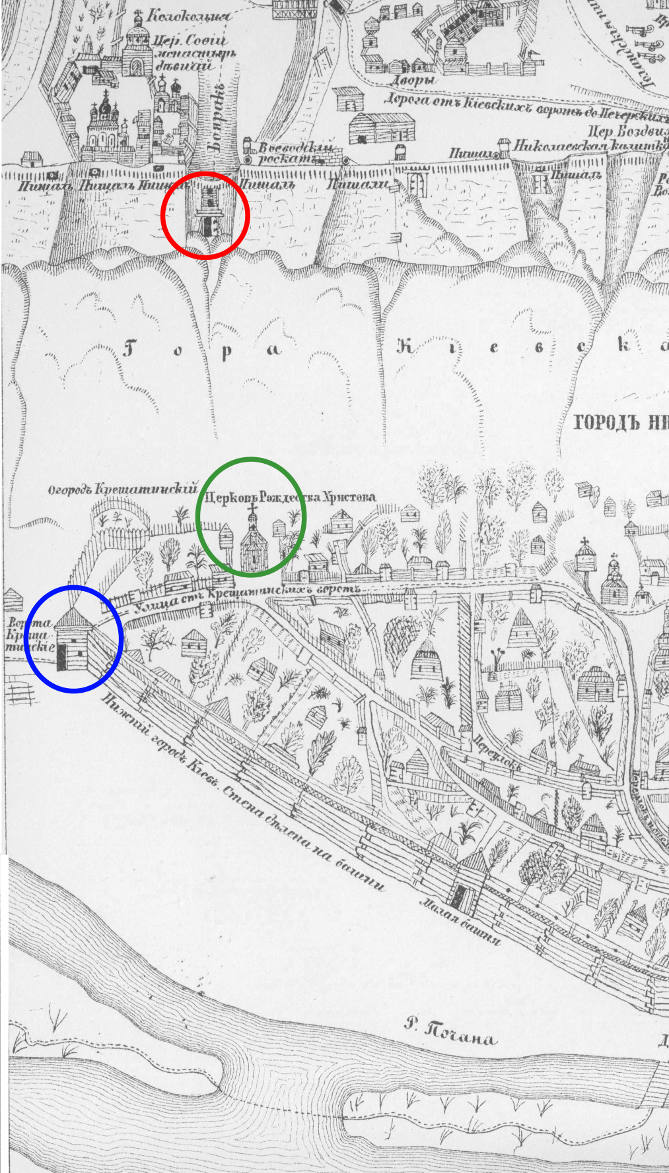
\includegraphics[width=0.60\linewidth]{chast-colebanie-osnov/pochayna/1695-kr.jpg}
\end{center}

На копии плана Ушакова я отметил красным – михайловскую калитку, зеленым – церковь Рождества Христова, синим – Крещацкие ворота. Местность налево от ворот до памятника Магдебургскому праву и есть крещацкая земля (она впрочем на картинку не поместилась). А между красным и зеленым кружками и надо полагать ввоз Михайловский, там же и Боричев.

Про Евсейкову долину в том же документе есть уточнение:

\begin{quotation}
отец наместник Сименон Шмигельский словесно сказывал, что та Евсейкова долина положение свое имеет: выехав из города верхнего Киева в ворота к печерскому на праву сторону по за кловом у яр, у якого яру где теперь навоз скидают, оная Евсейкова долина окончалась.
\end{quotation}

То бишь с одной стороны Евсейкова долина граничит с навозным яром около Клова, а по другую – с яром источника Хрещатика, близ Владимирской горки. Под эти границы подходит нынешняя улица Крещатик купно с Бессарабкой.

Но вернемся к оврагу Хрещатику и смежной с ним землей. Судя по документам, там находились не только провары да трактиры.
 
В деле Киевской городской канцелярии 1752 года «о пойманных польским ротмистром Рокицким двух разбойниках Григорие Киселенке да Григорие Пархоменке» приведены показания Ивана Сергеева, по прозвищу Кошин и Гончар, 27 лет: 

\begin{quotation}
он, Кошин,  после отца и матери обретался в оных же кожемяках у тамошнего жителя Ивана Плесуна, в гончарской науке лет 10-ть и более, а потом находился близ крещатской пристани, ведомства Киево-софийской катедры\footnote{Собора.} для делания кирпичей, где будучи на приставленной у оных кирпичей старостою Ивана Кучера дочери Агафии одружился; 

и в прошлом 1751 году, когда оный тесть его из оного Крещатика перешел на Лыбедь, ведомства Киево-софийской катедры к цегельням, для делания кирпича, то тогда и он с ним перешел [...]
\end{quotation} 

Из сего заключаю, что речь идет о двух кирпичных заводах. Один – в тогдашнем овраге Хрещатике или близ него. А цегельни на Лыбеди – вероятно цегельни в Протасовом яру, ведь мимо него протекает Лыбедь.

И кто знает точное место кирпичного завода на Хрещатике, и сколь много он постарался в уничтожении древнего склона при добычи глины? Что могло при этом погубиться? Ведь на Почтовой площади при устроении там еще при царе Горохе почтовой станции нашли древнее кладбище. Было таковое и выше.

На юго-восточном склоне холма, над лестницей к памятнику Магдебургскому праву, до 2014-го года находилась заброшенная, популярная в советские годы танцплощадка «Жаба»\footnote{50°27'19.18"N 30°31'45.45"E}. Снесли, годом спустя там уже был пустой пятачок. А над ним, еще выше – полукруглая смотровая площадка около арки Дружбы Народов. 

Сумбурная статья Ильи Михайловича Самойловского\footnote{Поныне не опубликованы, но келейно используются учеными два больших труда Самойловского, «Археологическая карта Киева (в расширенных его границах, до половины XIII в.)» и хроника «Археологічні дослідження на території м. Києва».} «Славянский могильник в Киеве над Днепром» в украинском журнале «Археология» (1950, №3) сообщает, что когда в 1935 году «планировали выступ над кручей» (устранили горб на краю), то в 19 метрах от края, на площади около 275 квадратных метров, в суглинке нашли более 30 скелетов разного пола и возраста. Они лежали на спинах, головами к западу, с вытянутыми вдоль туловища руками. В некоторых захоронениях обнаружили трухлявую древесину и ржавые гвозди, вроде от гробов, а также положенные в ногах у покойников украшенные узорами горшки, славянские и, как написано, «хазарского» типа. Останки перевезли в Институт археологии, где они пропали во время Великой Отечественной войны.

По ходу чтения статьи выясняется, что утёс срез\'али еще раньше, в 1896 году. Тоже нашли захоронения, предметы из которых отправили в московский Исторический музей. Сказано и о других языческих захоронениях подле того выступа, или утёса. Какой именно выступ имеет в виду сочинитель статьи – где смотровая площадка, или по месту «Жабы»? Самойловский указывает, что во время написания статьи (либо в 1935 году) там, на «выступе», находился павильон «Орианда».

\begin{center}
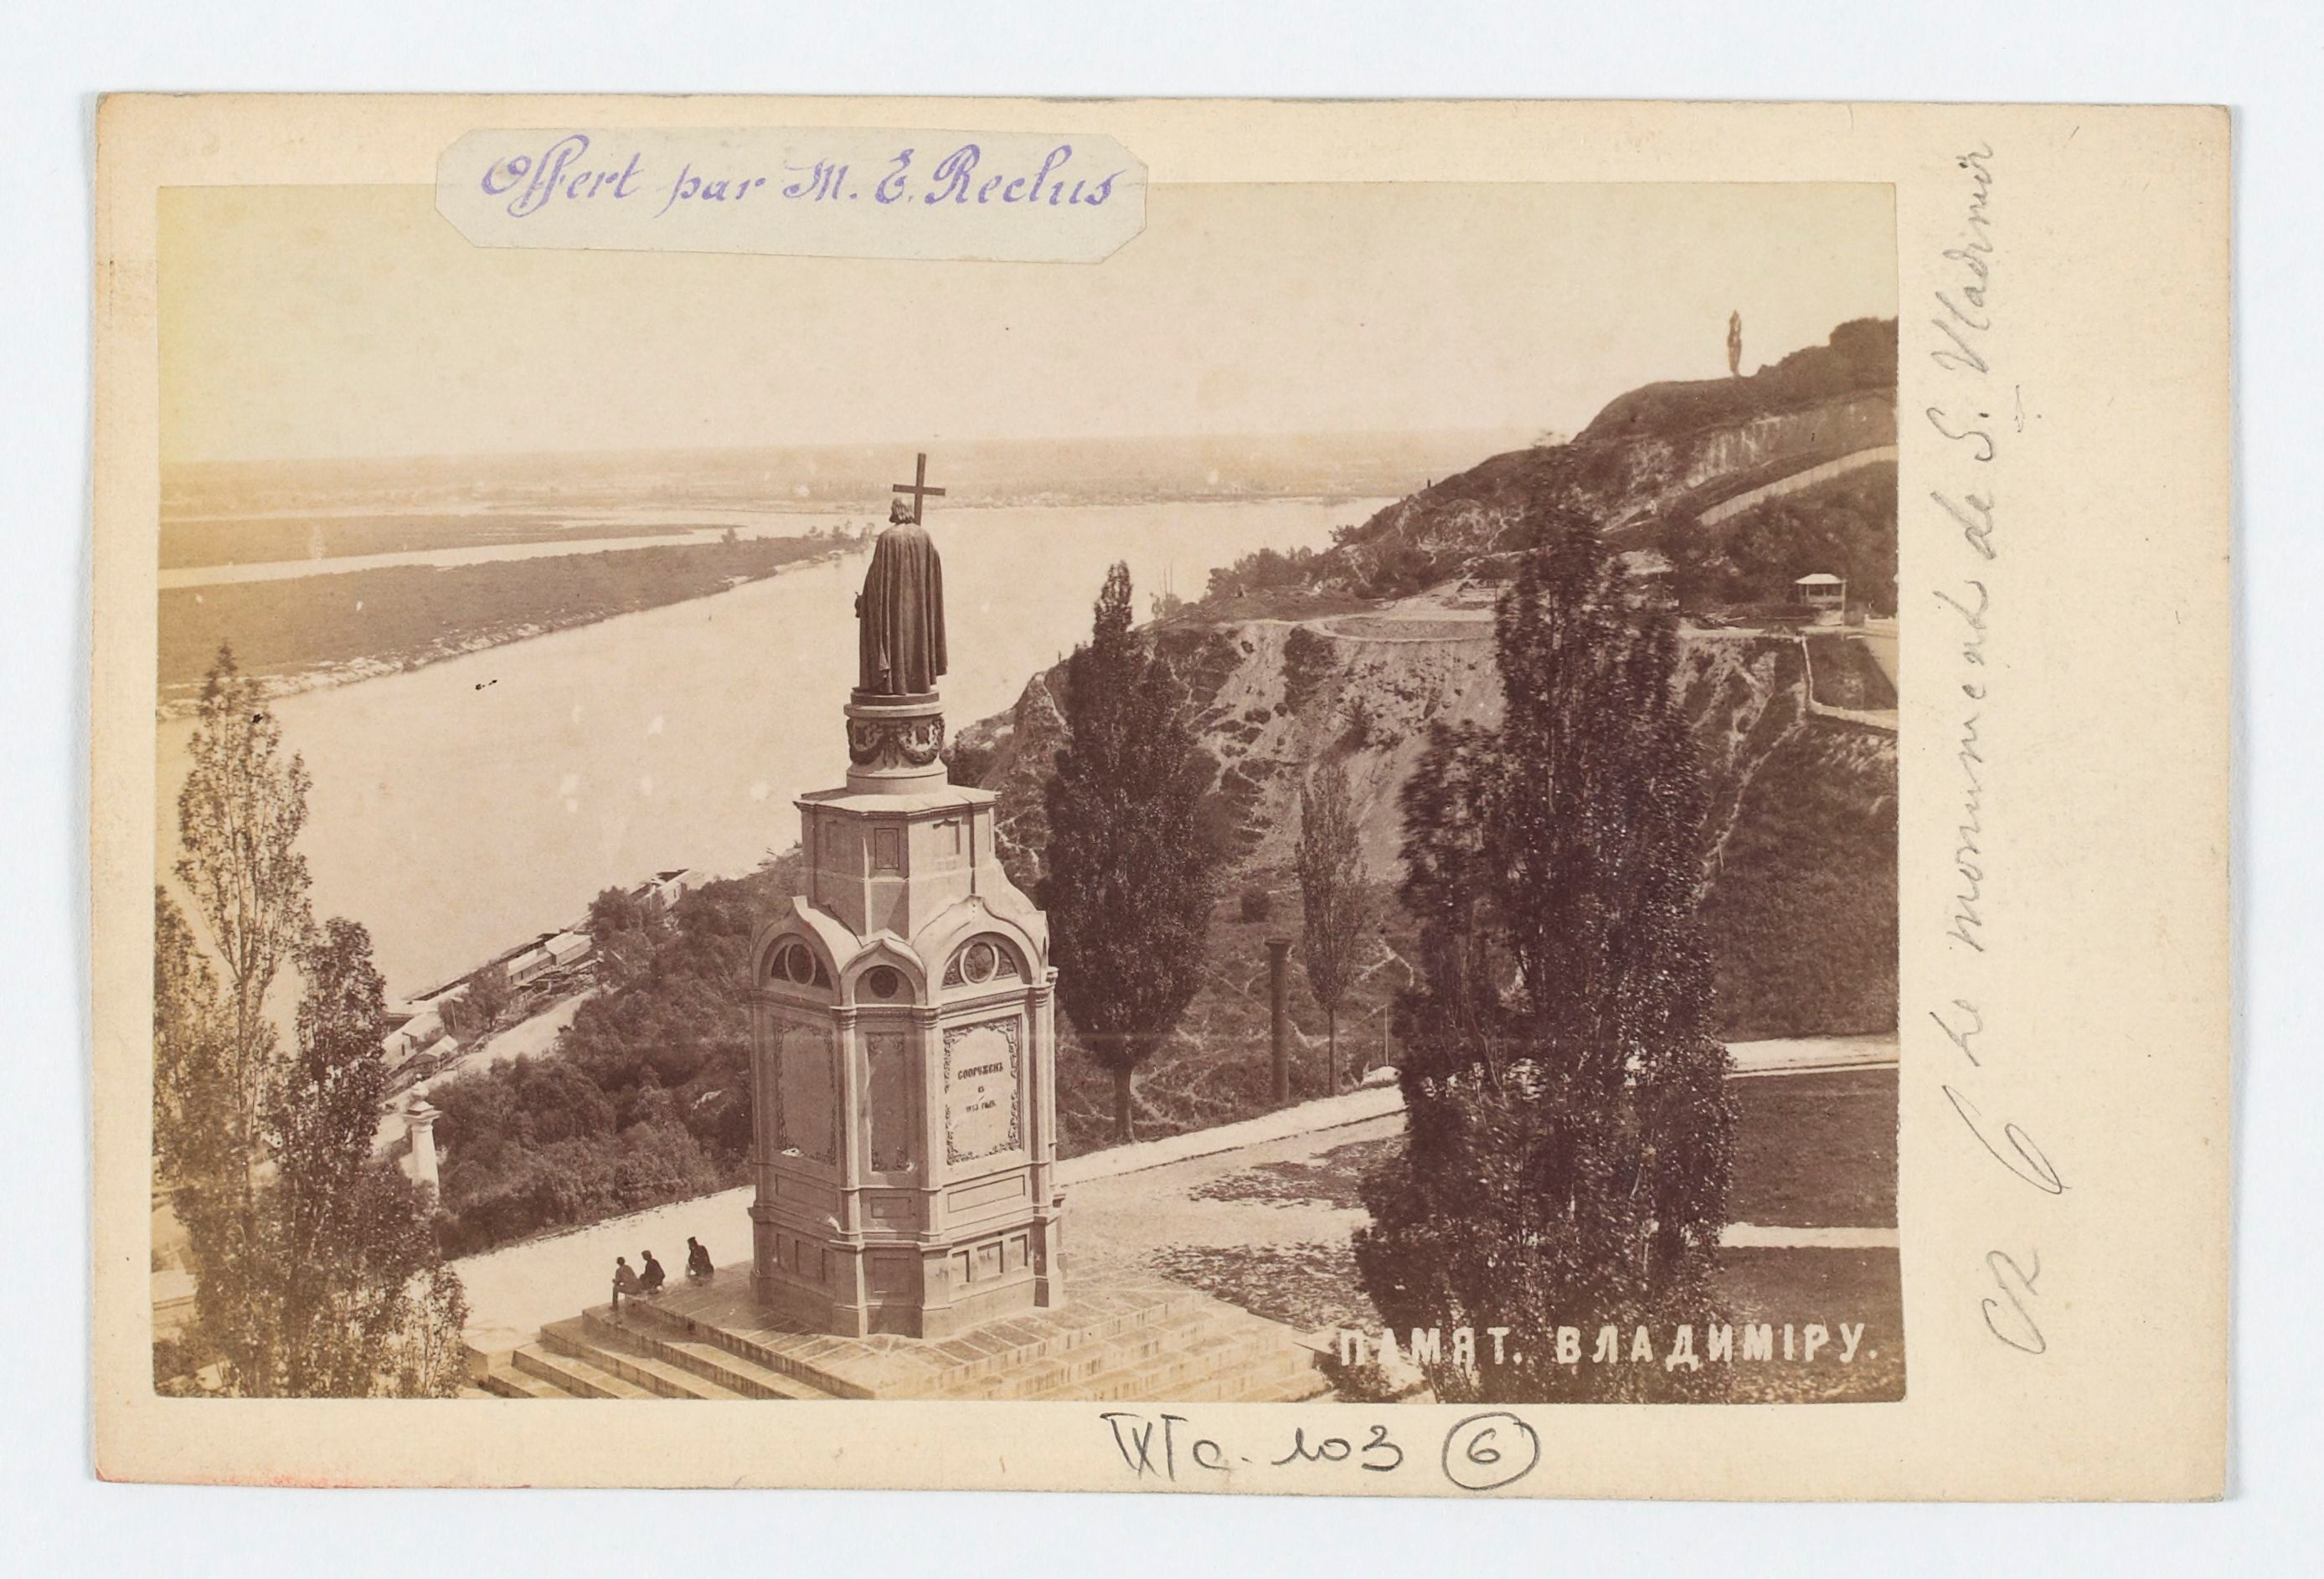
\includegraphics[width=0.94\linewidth]{chast-colebanie-osnov/pochayna/kupsob.jpg}
\end{center}

\begin{center}
\includegraphics[width=0.94\linewidth]{chast-colebanie-osnov/pochayna/\myimgprefix sadkup.jpg}
\end{center}

На этих дореволюционных снимках хорошо видно, как еще тогда верхушка склона срезалась неоднократно. Первая фотография сделана раньше, там плато на склоне еще не такое обширное. На второй – уже стоит павильон – «Орианда» ли, не знаю. Ниже слева видим площадку, где потом расположится «Жаба».

И еще левее будет овраг Хрещатик с одноименным ручьем. 

Его часто путают с ручьем, протекающим наверху, на улице Крещатик, под землей. Тот ручей является притоком Клова (Клов же, в свою очередь – приток Лыбеди). Вытекает примерно от Козьего болота, в окрестностях нынешней площади Независимости. Взят в коллектор. Диггеры называют его Крещатиком.

А Хрещатик исторический – на склоне. Его и притоком считать сложно. Ручей, свод родников из оврага, питаемый водоносным горизонтом Владимирской горки\footnote{Однако, не мог ли прежде ручей с Козьего болота протекать сюда?}.

Сейчас там проложена лестница от колоннады с Владимирского спуска вниз до набережной, к памятнику-колонне. Много лет эта лестница была в чудесном, вдохновляющем аварийном состоянии, в 2013 году её починили, с тех пор я по ней перестал ходить.

История колонны такова.

Закревский пишет, что

\begin{quotation}
с давних пор здесь существовал колодец, с небольшою над нею деревянною часовнею, украшенною иконами Св. Владимира, Святых мучеников Бориса и Глеба и другими. Часовня эта принадлежала к Подольской церкви Рождества Христова, и причт сей церкви два раза в год совершал крестный ход к колодцу Князя Владимира (так его звали) [...]
\end{quotation}

Не знаю, где был описываемый Закревским колодец – по месту ли изображенному на плане Ушакова, наверху, или же внизу. Скорее всего внизу.

В 1802 году горожане построили здесь по проекту архитектора Меленского кирпичный памятник в виде колонны Тосканского ордена, на арке, под которой поместили колодец, куда трубами провели воду. Закревский говорит:

\begin{quotation}
бывшая криница засыпана землею, а ключи от нея собраны в трубу и проведены в бассейн, устроенный несколько ниже ея под каменным павильоном, от чего вода может падать, в бассейн, в виде фонтана.

Павильон, заменивший собою убогую каплицу, был также украшен иконами, бывшими в ней, и по-прежнему оставался под ведением причта Христо-Рождественской церкви
\end{quotation}

На колонне были доски с надписями: «Святому Владимиру Просветителю России» и «Усердием Киевскаго гражданства за утверждение прав древния сея столицы Всероссийским Императором Александром I – 1802 года, сентября 15 дня». Речь идет о Магдебургском праве, которое Александр I подтвердил как действующее в Киеве. Впервые Киев получил это право в 1494 году от литовского князя Александра, а упразднено оно было Николаем I в 1834-м.

Российский Александр о памятнике был ни сном, ни духом, узнал про него задним числом, и в своем указе Киевскому военному губернатору Феншу от 7 ноября 1802 года хоть и похвалил местные власти за памятник Владимиру, но сурово удивился, что возведен он был без высочайшего ведома. Вскоре, уже с такового ведома, должность Фенша занял генерал Тормасов.

После постройки в 1853 году по проекту барона Клодта знаменитого Владимира с крестом на Владимирской горке, памятник-колонна стала называться «нижним памятником Владимиру». В 1861 году его несколько обновили, поскольку при земляных работах с 1843 года по обустройству набережной и Александровского (ныне Владимирского) спуска источник почти иссяк и пришел в запустение. Кроме того, в овраге и окрест вырубили деревья и снесли хижины бедноты.

Сверху вниз к памятнику раньше сходила лестница из деревянных ступеней. В 1915-м ее заменили на каменную, которую и отремонтировали в 2013-м. Если спускаться, по левую руку, на склоне между лестницей и Владимирским спуском, лежат здания бывшего заведения искусственных минеральных вод. 

\newpage

\begin{center}
\includegraphics[width=\linewidth]{chast-colebanie-osnov/pochayna/\myimgprefix 09.jpg}

\textit{Вид на овраг Хрещатик с Труханова острова.}
\end{center}

\begin{center}
\includegraphics[width=\linewidth]{chast-colebanie-osnov/pochayna/\myimgprefix alexspusk03.jpg}

\textit{Александровский (Владимирский) спуск. Арка в овраг с лестницей к памятнику. Слева выглядывает здание минеральных вод.}
\end{center}

\newpage
\vspace*{\fill}
\begin{center}
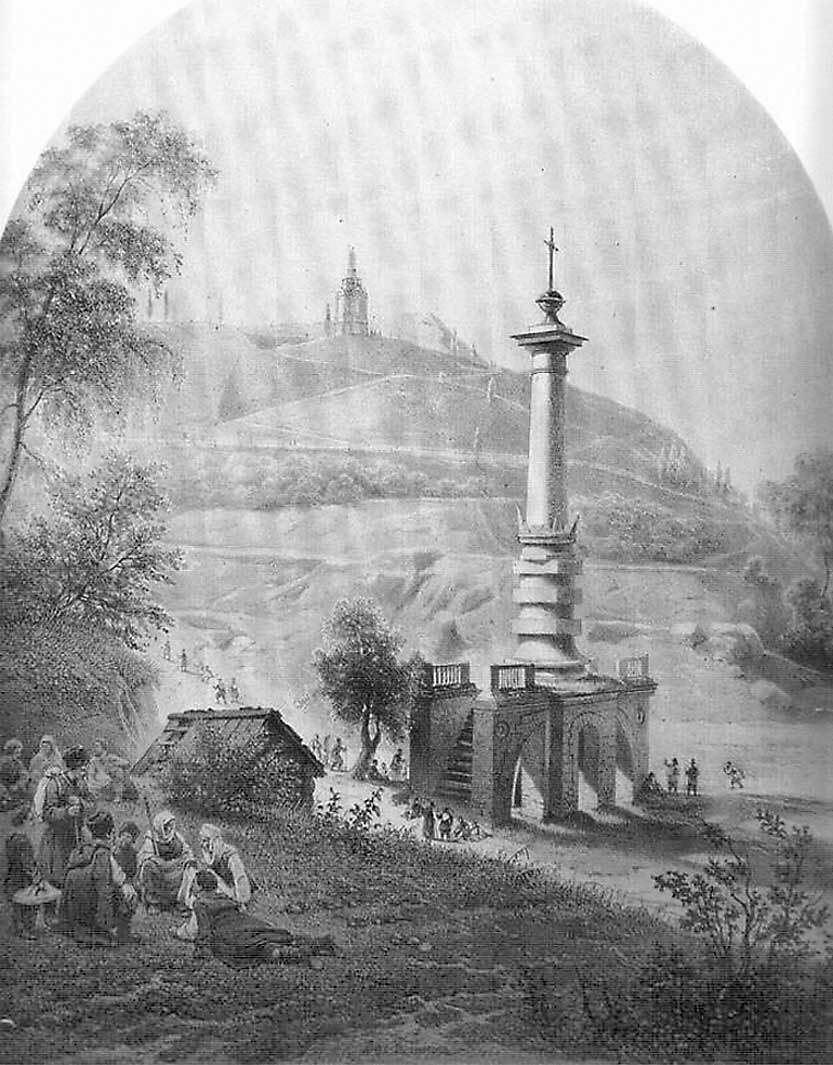
\includegraphics[width=\linewidth]{chast-colebanie-osnov/pochayna/nijn-vlad-01.jpg}

\textit{Картина Василия Тимма, 1862. Вид со стороны Днепра.}
\end{center}
\vspace*{\fill}
\newpage

\begin{center}
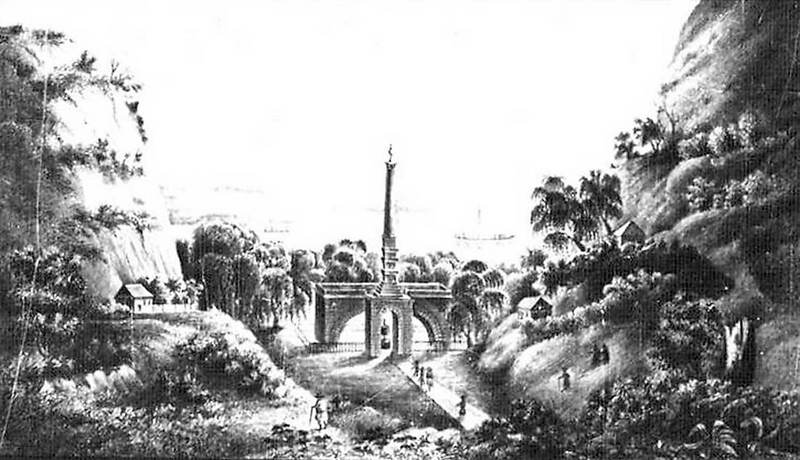
\includegraphics[width=\linewidth]{chast-colebanie-osnov/pochayna/1839-vadim-pasek-zakr.jpg}

\textit{Картина Вадима Пассека 1839 года, из книги Закревского, вид как если спускаться по лестнице к Днепру. Примечателен холм слева. Его уже нет, но был ли?}
\end{center}

\begin{center}
\includegraphics[width=\linewidth]{chast-colebanie-osnov/pochayna/\myimgprefix 12.jpg}

\textit{Вид с другой стороны. В середине 19 века в подобном буфете при памятнике действовал бордель.}
\end{center}

\newpage


\begin{center}
\includegraphics[width=\linewidth]{chast-colebanie-osnov/pochayna/\myimgprefix lestnica01.jpg}

\textit{Деревянная лестница, бывшая тут до 1915 года.}
\end{center}


\begin{center}
\includegraphics[width=0.60\linewidth]{chast-colebanie-osnov/pochayna/\myimgprefix lestussr.jpg}

\textit{Уже каменная. Снимок времен СССР.}
\end{center}

\newpage

\begin{center}
\includegraphics[width=\linewidth]{chast-colebanie-osnov/pochayna/\myimgprefix IMG_1429.JPG}

\textit{2011 год.}
\end{center}


\begin{center}
\includegraphics[width=\linewidth]{chast-colebanie-osnov/pochayna/\myimgprefix IMG_1403.JPG}

\textit{2011 год.}
\end{center}

\newpage

Родники, питавшие источник Хрещатик, поныне текут в дренированных склонах и по бетонным желобам в оных. Откуда именно пил воду Максим Берлинский, я не знаю, однако он признал ея непригодной к употреблению и назвал вкус «охренным». Среди народа же водица из Хрещатика слыла исцеляющей глазные болезни. Я попробовать воду тамошних родников не рискнул, ибо видел на склонах осязаемые следы человеческого пищеварения.

Вероятно, место это в прошлом было столь же волшебно, как удолье Выдубицкого монастыря. Длина лощины Хрещатика в лучшие времена едва ли составляла более 80 метров – это яр не столь глубокий, как допустим Репяхов или Бабий. 

Но вот и все притоки Почайны, первой и второй. Почему я уделил им много внимания? От судьбы притоков зависит судьба реки, а значит понимание исторических событий, с нею связанных.

Исследуем вопрос о глубине и ширине Почайны. Ответить на него можно только с указанием времени и места. И то не всегда. Про судоходность я уже писал – раньше корабли могли плавать едва не в лужах. Однако глубина Почайны была достаточно смертельной по крайней мере в 17 веке около Щекавицы.

В отписке воеводы Василия Шереметова о приходе под Киев полковника Данилы Выговского, за 7 октября 1658 года\cite[том 15, стр. 258]{akty} писано:

\begin{quotation}
и обоз Павла Ененка взяли и знамена и пушки все поимали и черкас многих побили и поимали, а остальные черкасы все побежали и топились в речке Почайне, и многие потонули; а Щековица от города менши полуверсты.
\end{quotation}

Ширина Почайны. На плане Ушакова Почайна-1 выглядит третью ширины Днепра, а Почайна-2 – то третью, то – на уровне Почтовой площади – равна ему Днепру. На плане Шуберта, Почайна-1 ниже впадения в нее Сырца, шириной подобна равнинной реке среднего пошиба вроде Сулы, а после соединения с нею Чернечьего озера – и Ворсклы.  

Былины донесли любопытное предание о богатырской забаве на Почайне. Почайна в былинах называется по-разному – то Пучай-рекой, то Пучайкой, то просто Почайной. А у богатырей были особые лошади с кожаными подкрылышками. Чем больше этих подкрылышков, тем дальше скачет конь. И вот богатыри соревновались, перепрыгивая Почайну на своих чудесных скакунах.

Поделюсь мыслями об изменениях Почайны-1 и Оболони. Гидронамыва при строительстве жилмассивов, совершенно преобразившего местность, я и касаться не буду.

%О распаде реки на долгие участки, ставшие праобразом современных озер Кирилловского и Иорданского (мне не надоело постоянно напоминать, что старые одноименные озера были в другом месте, вне русла Почайны). Ведь хорошо прослеживаемое на картах 19 века русло Почайны – это цепь долгих водоемов, связанных ниточками ручейков или каналов. Карты не сообщают, что это за соединительные нити.

%\begin{center}
%\includegraphics[width=\linewidth]{chast-colebanie-osnov/pochayna/1846-po.jpg}
%\end{center}

%Примерно на участке русла, отмеченном синим овалом, ныне Богатырское и Кирилловское озера, красным овалом – современное Иорданское.

О распаде реки на долгие участки. Почему Почайна была перебита пополам примерно в районе устья Сырца?

Вот у нас в седую древность есть водоток Почайны, с севера на юг. Он силен и течет ровно. Со стороны в него впадает весьма быстрый Сырец. Он, как и любая река, несет не только воду, но и твердые частицы грунта (чем быстрее течение, тем меньше частиц оседает на дне и тем больше перемещается дальше). Но вода главного потока достаточно сильна и, подхватив частицы, тянет их дальше на юг.

Главный поток, выше устья Сырца, по ряду причин ослабевает. А Сырец продолжает нести грунт. Главный поток уже не в силах увлекать его в сторону как прежде. Возникает обмеление. Как видно по картам 19 века, прерывание широкого русла Почайны возникало там, где к нему подходили притоки – то Сырец, то старое Иорданское озеро, наконец Глубочица тоже своей мутью приложила руку.

Что еще влияло на Почайну?

Устроение во второй половине 19 века мостов через Днепр в районе Киева привело к местному углублению русла Днепра. Дно опустилось, а с ним и поверхность воды. Ниже уровень – больше уклон притоков, в том числе Почайны-1. Больше уклон – увеличение скорости течения. Но воды-то в Почайне-1 не прибавилось от того, что Днепр стал «залегать» ниже. Усилилось обмеление частей Почайны – уровень воды в ней снизился за счет увеличения скорости, а не количества воды.

Железная дорога. В 1916-1917 годах через Днепр на широте нынешней Петровки да залива Волковатого перебросили железнодорожный мост императрицы Марии Федоровны, позже Петровский. Подведенная к нему линия железной дороги нарушила из без того извращенную человеком водную систему и привела к заболачиванию местности к северу от насыпи с рельсами. Еще ранее, в начале 20 века, севернее этой железной дороги, существовала узкоколейка Общества дубильных экстрактов, проведенная от Куренёвской площади (южная часть современного Куренёвского парка) через Почайну-1 и до залива Старика (Пробивицы) – это примерно микрорайон на юго-восток от станции метро Минская.

Водяные мельницы и винокурни. Давние земельные грамоты ничего не говорят про мельницы и винокурни на Почайне. Они были на ее притоках – Коноплянке, Сырце, Глубочице. 

По крайней мере с 17 века люди заводили водяные мельницы. Зимой они не работали – вода-то замерзает. В студеную пору мололи на ветряных либо ручных.

Основа водяной мельницы это колесо с лопастями. Есть три вида таких колес, различных по принципу работы – и коэффициенту полезного действия. 

Самое простое колесо – подливное. Оно просто опущено в поток воды, который вращает колесо. 

Второй тип – среднебойное колесо. Оно похоже на подливное, но используется перепад высоты. С верхней точки вода льется по уклону вниз, проходя под колесом и вращая его.

Наконец третий тип, самый действенный – наливное колесо. Ему тоже необходим перепад высоты, но вода идет не под колесо, а льется на лопасти сверху. Мельницы с колесами второго и третьего видов требуют наличия плотины для создания перепада высоты. Такие плотины строились во множестве, как видно по картам и документам. Гребелька там-то. В пруде над плотиной разводили рыбу, а по берегам гуще росла трава.

Весной плотины надо было разбирать, чтобы пропустить лед и вешнюю воду. Если не сделать этого, плотину прорвет и вниз пойдет водяной вал, снося гребли дальше по течению. Иногда мельники-соперники тайно, ночью сами вызывали такой прорыв, чтобы наказать мельницы ниже. И списывали на силы природы.

Как влияет плотина на реку? Вот у нас плотина. Выше её течение замедляется, глубина увеличивается, в образовавшемся пруде постепенно оседают наносы, крутые берега обваливаются и превращаются в пологие, повышается уровень грунтовых вод, окрестности постепенно заболачиваются. Ниже плотины, русло размывается, дно опускается, уровень грунтовых вод понижается (колодцы пересыхают).

Сырец, во времена рьяного освоения его человеком, почти на всей протяженности был цепью больших прудов – то монастырских, то хуторских. Что ни хутор, то свой пруд. Несколько веков в реке поддерживался искусственный режим течения. Пруды увеличивали количество наносов, поэтому при выходе на равнину Куренёвки и Оболони, Сырец мелел, растекался вширь, заболачивал окрестности. Помимо постоянного действия мельниц, были и другие ощутимые вмешательства человека. Мы помним, как крестьянин раскопал русло и Сырец от этого изменил своё течение.

Винокурни. Просто испаряли воду. Винокурня ведь не относится к виноделию, а является эдаким большим самогонным аппаратом. Вином (хлебным или простым) раньше называли почти то, что нынче считается самогоном, а водкой на Руси именовалось уже переработанное, вышеупомянутое «вино».

Современные винокурни (выпускают виски) в странах вроде Шотландии летом, когда уровень рек небольшой, прекращают свою работу, чтобы не понизить его еще более. Как видно по документам 17-18 веков, владельцам винокурень это было пофиг, пока не стали жаловаться мельники, ибо работа мельниц на иссякающей реке затруднительна. Название района Куренёвки, лежащего при Почайне-1 и Сырце, красноречиво свидетельствует о прошлом занятии здешнего населения.

То же и Приорка – в давних документах она часто обозначена как Проварка (Приварка), от «проваров», пивных заводов, хотя общепринято производить название от слова «приор» – настоятель католического монастыря. Сие толкование также справедливо.

Почайна, Оболонь и поля орошения.

В 1890-е в окрестностях Приорки, Куренёвки и Оболони – с одной стороны вдоль низовья Коноплянки и севернее её, а с другой стороны вдоль Кинь-Грусти, поглотив часть речки Мушанки – люди устроили поля орошения (160 десятин), а также канализационные луга (100 десятин). Нечистоты городской канализации со всего правого берега Киева направлялись по трубам на эти поля, чтобы очищаться естественным образом. Природа всё схавает! На полях орошения выращивают овощи. 

Спустя двадцать лет канализацию расширили, а поелику существующие поля орошения с таким объемом поступлений справиться не могли, было решено – сбрасывать на прежние поля лишь отходы с Подола и районов севернее оного, а говно с остальной части города направили просто в Днепр, устроив сброс возле устья Лыбеди. Так продолжалось до 1965 года.

С полей орошения тоже есть стоки, но их объем незначителен, их спускают куда ни попадя. Что до именно наших полей, то они заняли место, где раньше был водоток от верховий Почайны-1 (Улуково-Министерка) и на юг эдак до широты Пробивицы.

Судьба острова Чачина. Газета «Киевлянин» в 1910 году писала:

\begin{quotation}
Со времени введения в 1870 году городского положения, городские земли Киева оставались без ревизии, без контрольных измерений. При таких условиях, путем постепенных незначительных изменений, границы огородов, сенокосов и пахотных земель перестали соответствовать остававшимся без изменения планам на эти земли. Наглядным примером этому может служить изменение фигуры Труханова острова, где общая площадь уменьшилась на 14 десятин\footnote{15,2 гектара.}, благодаря тому, что водами р. Днепр отмыта часть острова. Водами р. Днепр также почти уничтожены городские земли под названием «урочище Раф», мерою до 6 десятин\footnote{6,5 гектара.}. С другой стороны, у острова Чичина образовался примывок, размером до 10 десятин\footnote{10,9 гектара.}, остававшийся до текущего года совершенно не нанесенным на план города. 
\end{quotation}

Чачин исчезал, кажется, быстрее, чем рождался. Широкий ныне залив Собачье гирло раньше был узким проливом на этом острове. Добыча песка в заливе расширила его, сожрав часть Чачина. А ведь в 1975 году на косе Собачье гирло, в южной ее части, около причала «Охотничья станция 2», при расчистке фарватера Днепра со дна подняли один из так называемых священных дубов – дуб со встроенными в него кабаньими челюстями.

В дубе вырез\'али дыру, вставляли туда челюсть зубами наружу, потом посередине дыры вбивали кол, он обрастал, и получалось, что из коры просто торчат зубы. Таких челюстей в дубе насчитали десять. Ученые присудили этому дубу возраст 2000 лет, и решили, что тысячу из них он пролежал в воде. Ныне дуб хранится в музее в Пирогово.

Полагают, что такие дубы связаны с культом Перуна – мол, и дрова около идола Перуна дубовые жгли, да в не имеющей отношения к Киеву земельной грамоте 1302 года галицкого князя Льва Даниловича написано: «а от той горы до Перунова Дуба горе склон бысть владениям епископа Перемышльского». Давняя связь язычества с дубами вырисовывается набросками, без видимости общей картины. Дрова, урочище... Но священным деревом громовержца Зевса считался тоже дуб.

В Голосеево есть поляна\footnote{Примерно тут: 50°22'49.0"N 30°29'56.4"E, на юго-запад от дома по адресу Сельскохозяйственный переулок, 1.}, где правильным кругом стоят могучие дубы примерно одного возраста. Кстати, высаженные кругом дубы возле Улукова хоть потоньше голосеевских, зато непосредственно выше по течению от Собачьего Гирла, и как знать древность той дубравы?

%Однако не вижу оснований называть дубы с встроенными челюстями – перуновыми, равно как нет предпосылок понять назначение этих челюстей в дереве. Строить догадки – пожалуйста, сколько угодно, а вот логически выстроить цепь не получится, мало данных.

Название и очертания острова Чачина сохранялись до тридцатых годов двадцатого века. Картографы последующих десятилетий, кажется, не интересовались этой местностью. Раньше там ведь сено косили. А в город пришел железный конь. Не нужны стали луга и забылся остров. Потом Оболонь начали перекраивать строительством жилых массивов Минский и Оболонь. С другой же стороны, от Кирилловских высот, подползла промзона.

В сборнике «Чтения в историческом обществе Нестора летописца. Книга 1. 1873-1877» я нашел любопытные сведения, относящиеся к Подолу и Оболони. 

На одном из заседаний общества протоиерей Лебединцев докладывал о планах Киева 1706 и 1728 годов, хранящихся в Петербурге. Лебединцев снял с них копии и предъявил собравшимся. В издании планов нет, взамен даны словесные примечания. Они столь познавательны, что приведу их целиком:

\begin{quotation}
Копии с двух древнейших из вышеозначенных планов г. Киева, именно планов 1706 и 1728 г., снятыя протоиереем Лебединцевым в бытность его по службе в Петербурге, предъявлены в том же заседании с объяснением их особенностей, касающихся истории Киева.

Любопытно было видеть на этих планах, что в 1706 г., Крещатик и Липки еще состояли из пашен монастырских; со Старого Киева на Подол еще существовала дорога по Боричеву взвозу; у Христорождественской церкви был небольшой, до 75 саж. длины, залив Днепра, между материком Днепра и мысом нынешняго набережного шоссе;

Подол отделялся от Оболонья ручьем, от 10 до 16 саж. широты\footnote{21-33 метра. Для сравнения – ширина шоссейной части Крещатика у перекрестка с Прорезной – около 24 метров.}, который с Кожемяк, от Крестовоздвиженской церкви, направлялся через площадь нынешняго Житнаго базара под Щековицею и потом близ юрковицкаго моста по Оболонью, с северной стороны Подола, за большим ретраншементом\footnote{В фортификационных сооружениях – вспомогательное, внутреннее ограждение либо два окопа с валом между ними.} до впадения в Днепр канавы, разделяющей ныне Подол на Подольскую и Плосскую части.

Для г. Киева и Х округа путей сообщения преимущественно может быть интересен план Киева 1745 года с промерами днепровскаго форватера у Подола. 

Из того же плана видно, что на протяжении от Ильинской церкви до впадения Почайны в Днепр\footnote{От Ильинской на север к устью Почайны-1, или подразумевается таки Почайна-2 с устьем на юг от упомянутой церкви?}, было до 31 мельницы, прикрепленных к паромам\footnote{Речь идет о «лодейных» мельницах, где колесо с лопастями крепилось к лодке либо к иному плавучему средству.}, близ правого берега, и что течение Днепра здесь имело от 80 до 90 саж. в минуту\footnote{168-189 метров в минуту.}. 

Для защиты Подола от напора днепровского течения, после 1745, прорыт материк, отделявший Днепр от р. Черторыя, и теперь с трудом проходят плоты к Оболонью, где быстро работали колеса мельниц\footnote{Сопоставление мельниц с Оболоньем – не привязка ли вышеупомянутой Почайны к Оболони? Если да, речь шла о Почайне-1.}.
\end{quotation}

Про «за большим ретраншементом» – разгадка исчезновения Глубочицы на прорисовках плана Ушакова в районе Подола. Глубочица отклонялась ранее к северо-восточному подножию Щекавицы. А вдоль него же идет, затем поворачивая к Почайне, и крепостная ограда на плане Ушакова. Ограда эта следовала рядом с руслом Глубочицы, неясно лишь, по какую его сторону. Итак, Лебединцев словесно описал былое русло Глубочицы начиная от Кожемяк. 21-33 метра ширина – неплохо. Чем, кстати, не Притыка? И Дебоскет именует Притыкой нечто, длящееся от Крестовоздвиженской церкви до Днепра. Совпадает.

При изучении Почайны передо мною встал не один трудный вопрос, и на многие я не нашел ответа. С чем я столкнулся? 

Первое. Не могу разобраться, что значит слово «почайна». Существует город Почаев. В Новгороде тоже есть река Почайна, теперь взятая в коллектор.

Возможно, «почайна» это искаженное «пучина». Или, «почайна» – это вроде украинского слова «пошана» (почёт). Существовало сходное русское слово «почтенья», означающее оказание почестей идолам. Идолы стояли на холме и проплывающие могли, завидев оные, воздавать им хвалу. 

Либо «почайна» от слова «почивать» – покоиться, отдыхать. А может, есть какой-то общий корень у острова Чачина, птицы чайки и речки Почайны. Еще – Почайна (Почана) легко превращается в Бочайну, Бочану – Боковую, она сбоку течет, либо связана с бочками, которые могли бы выгружать по ее берегам.

Либо Почайна это искаженное «песчаная». На плане Ушакова она пишется как «Почана» – весьма близко к этому.

Я обратил внимание на близость звучания слова «Почайна» с Пуща и Буча. А ведь поблизости у нас – Пуща-Водица и Буча. Буча это ведь тоже искаженное «Пуща». Слово «пуща» имеет несколько значений. Это и просто густой лес, заросли (вспомним английское «буш», тоже лес). Но также это лес заповедный, охранный, его не вырубают, берегут.

Кстати, в старину Болонью и Оболонью называли окраину города. Болон значит край. Другие значение слово «болонь», по Далю: «низменная луговая равнина у реки или  озера; выгон, толока, поскотина». Все эти значения сплошь подходят, ибо и окраина города, и низменная луговая равнина, и выгон, где скот пасли. Замечательно!

Далее про именования.

В земельных грамотах и картах названия местностей меняются не просто от года к году, но и в зависимости от составителя карты или документа. Разные люди в одно время могли называть ту же местность по-разному.

В одном протоколе действий межевой комиссии упомянуты речки Мушанка и Тушанка. Судя по описанию местности, речь идет об одной реке. И название отличается всего буквой. В документе нет никаких пояснений на этот счет, что наводит на мысль о вероятности существования в любом документе «двойных» именований, о тождественности которых можно лишь догадываться.

При работе над этой главой я настолько погрузился в изучение, что ни о чем больше не мог ни думать, ни говорить. Обложился картами, документами, мне снились то накладывающиеся друг на друга русла, то полуостров на Почайне, населенный прокаженными (тогда я читал забытый еще при СССР роман Шилина). Огромного напряжения задало мне устье Ирпеня на старинных картах.

С этой странностью столкнется любой, кто начнет разбираться в прошлом Оболони и Почайны. На картах 17 и 18 веков, река Репин, она же Ирпень и Пирная, упорно изображается впадающей ниже Вышгорода. Впрочем, в 18 веке появляются и «правильные» карты, где Ирпень впадает выше, как сейчас. Например, на карте Днепра авторства Дебоскета за 1742 год устье Ирпеня находится южнее селения Демидово.

А если Ирпень раньше действительно впадал южнее Вышгорода, и затем сменил русло – или было два устья, одно севернее Вышгорода, другое южнее? Потом первое осталось, а второе превратилось в невесть что. Я принялся изучать карты и запутывался дальше.

На 17 века боплановской карте Ирпень впадает южнее Вышгорода, и неподалеку есть Karpilowka (на одном из вариантов Korpilowka). В те годы в земельных документах наиболее часто упоминается та Карпиловка, что поныне находится на левом берегу Днепра, на правом Десны, близ Остра – и точно застолблена там описаниями по смежным селениям, Лутаве и Выползове.

Существует и другая, гораздо меньшая Карпиловка около реки Ирпень, а не так далеко от нее на запад, в зоне отселения – тоже Карпиловка, заброшенный поселок. Какая Карпиловка была на старинных картах?

Многие сёла называются Руднями – значит, там  добывали руду. В многочисленных Гутах производили стекло. А была профессия корпийщиков, заготавливающих корпию – по Далю, это «растеребленная ветошь, ветошные нитки или нарочно выделанная пушистая ткань, для перевязки ран и язв».

И вот в документе «Решение о разграничении земель города Киева» 1701 года я нашел слова, на которые раньше не обращал внимания:

\begin{quotation}
Аби люде, на подворках Карпиловкою прозываемых, близко места Киева, от монастыра паненского Иорданского и от монастыра Кирилского мешкаючи, по самый поток, межи горами Шкавицей и Лисою\footnote{Под Лысой горой подразумевается гора, слывущая ныне Юрковицей.} будучи, належали непременно до монастыра Кирилскаго
\end{quotation}

Что это значит? Подворки – пригород. Пригород Карпиловка находился около «места» (города) Киева, в Карпиловке этой жили люди, относящиеся к монастырям Кирилловскому и Иорданскому. И решено было – люди, живущие от Карпиловки и до потока между Щекавицей и Лысой горой, «приписывались» к Кирилловскому монастырю. 

Следовательно, Карпиловка находилась около Кирилловского монастыря, от него и по Юрков поток. 

А ведь сейчас, через дорогу к севе\-ро-западу напротив Кирилловской церкви, начинается урочище Копылово и улица Копыловская! Название весьма похоже на Карпиловку, это не может быть совпадением. Копыловская улица известна с первой половины 19 века и, как гласит справочник, название её произошло от урочища Копыл. Я уверен, что раньше где-то здесь была Карпиловка. Искаженное ли это иное, прежнее название, приведенное к более привычной Карпиловке, или параллельное название давнего урочища – об этом мы порассуждаем позже.

На карте 1650 года Карпиловка нарисована точно на цепи гор Кирилловских высот, между Киевом и Вышгородом, и река Репин южнее Карпиловки протекает в сторону Днепра между холмами. Сопоставляя с современной местностью, полагаю, что «картографический» Ирпень мог протекать по одному из глубоких яров – Репяховому или Бабьему.

Мой разум сопротивляется, объявляет это фантастикой, ему удобнее думать, что на картах просто ошибка, которая копировалась с одной карты на другую, а затем, с течением лет, постепенно исправлялась. Хотя Андрей Целларий\cite{sbornikmat} в середине 17 века пишет, безо всякой карты, словами, что Вышгород лежит ниже устья Репина.

\begin{center}
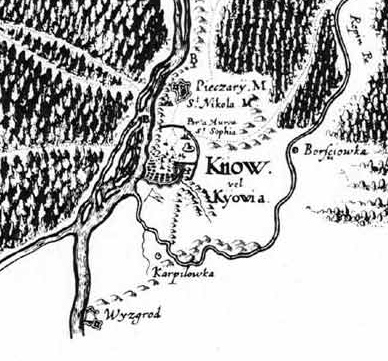
\includegraphics[width=\linewidth]{chast-colebanie-osnov/pochayna/1650-repin.jpg}

\textit{Карта 1650, ориентирована на юг.}
\end{center}

Известен роскошный атлас фламандского географа и картографа Абрахама Ортелиуса, Theatrum Orbis Terra\-rum, первая редакция коего вышла в 1570 году, а последующие выпускались при жизни Ортелиуса. На одной из карт этого атласа Видим Kiof (Киев) и два Visegrod (Вышгород) – один ниже по течению Днепра, другой выше. И между этим вторым Вышгородом и Киевом, в Днепр тоже впадает некий приток. Что это?

\begin{center}
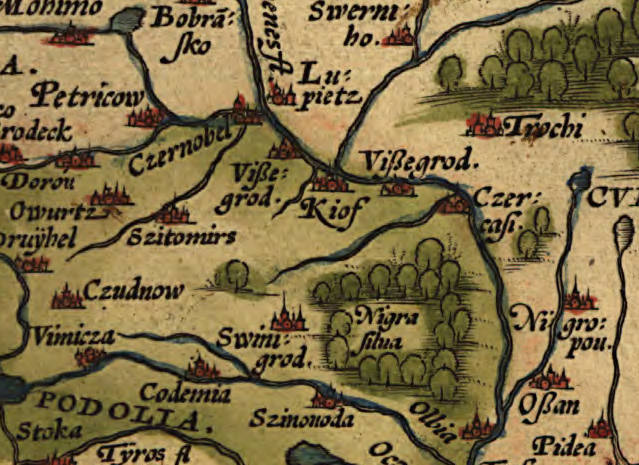
\includegraphics[width=\linewidth]{chast-colebanie-osnov/pochayna/1570-map.jpg}

\textit{Кусок карты Ортелиуса.}
\end{center}

На карте «Карте Киевского наместничества», 1792 года, тоже два Вышгорода. Первый классический, известный поныне – подписан «Выше городок», и другой Вышгород обозначен севернее, между Сухолучьем и Лютежем. Чуть южнее этого второго Вышгорода, по карте 1792 года, впадает Ирпень. Современный Ирпень тоже впадает в Днепр, водохранилище, примерно между Сухолучьем и Лютежем. Так может, был таки второй Вышгород?

А на карте «Малороссии, разделенной на наместничествы» (что случилось в восьмидесятые годы 18 века) показаны, на правом берегу Днепра, выше устья Десны – «Вышь Городок», и севернее его, но южнее Новосёлок – «Нижегородок», подписанный столь же крупно, как Белгородка и Борисполь. А «Вышь Городок» – мелко как Пуховка и Княжичи.

Ирпень не отпускает меня. Что-то странное связано с ним. Судите сами – другие реки впадают в Киевское море обычным образом, а воду Ирпеня, чей уровень ниже днепровского, в устье приходится поднимать насосами. Этим занимается Ирпенский гидроузел. Конечно же это объясняется поднятием уровня воды в Киевском море относительно уровня незапруженного Днепра в том районе, но остальные речки вроде бы впадают обычно.

До устроения Киевского моря устье Ирпеня было разумеется естественным, несколько восточнее затопленного ныне водохранилищем села Борки\footnote{50°44'29"N 30°23'54"E}, что лежало на восток от Козаровичей. Восточная часть прежних Козаровичей тоже ушла под воду, а западная уцелела и развитие села пошло на запад, туда, на материк.

Пойма Ирпеня, ныне дренированная, еще в первой половине 20 века была сильно заболочена и эта ее заболоченная, весьма приличная ширина выдается в Ирпене реку некогда гораздо более могучую, чем сейчас. Возможно, Ирпень, на Киевщине, прежде был так же широк, как нынешний Днепр в районе Киева.

А к Копыловке мы еще вернемся! Через несколько не глав, но частей.

%Название Ирпеня, Репина, кажется говорящее – в нем слышу я «Препин», препинание, препону.

%В 2016 году нависла угрозы застройки части (во многом рукотворной) открытого нынешнего русла Почайны-1 между Московским проспектом и улицей Электриков – речь идет об окрестностях залива Волковатого. Там канал от современного Иорданского озера и дальше сам заболоченный залив. По воде это Почайна-1, по местности –  прежде в разные времена там частично проходили  русла Почайны-1 и Днепра, однако это единственный участок вне раздутых озер Опечени, где остатки реки в современном ее русле хоть как-то оживляют природу. 

%Летом 2016 года этот участок реки расчищен людьми, неравнодушными к судьбе реки, они же вступили в противостояние с застройщиками.
